\documentclass[12pt]{article}
\usepackage{fullpage}
\usepackage[utf8]{inputenc}
\usepackage{pict2e}
\usepackage{amsmath}
\usepackage{enumitem}
\usepackage{eurosym}
\usepackage{mathtools}
\usepackage{amssymb, amsfonts, latexsym, cancel}
\setlength{\parskip}{0.3cm}
\usepackage{graphicx}
\usepackage{fontenc}
\usepackage{setspace}
\usepackage{gensymb}
\DeclareMathOperator{\dom}{Dom}
\DeclareMathOperator{\me}{Me}
\DeclareMathOperator{\mo}{Mo}
\DeclareMathOperator{\dt}{det}
\DeclareMathOperator{\cov}{Cov}
\DeclareMathOperator{\Exp}{Exp}
\DeclareMathOperator{\Var}{Var}
\DeclareMathOperator{\rot}{Rot}
\DeclareMathOperator{\Sop}{Sop}
\DeclareMathOperator{\rg}{rg}
\DeclareMathOperator{\arctg}{arctg}
\DeclareMathOperator{\diag}{diag}
\usepackage{adjustbox}
\setstretch{1.5}
\usepackage{bold-extra}
\usepackage{subcaption}
\graphicspath{ {images/} }
\usepackage{tcolorbox}
\usepackage{xcolor, colortbl}
\usepackage{wrapfig}
\usepackage{empheq}
\usepackage{array}
\usepackage{parskip}
\usepackage{arydshln}
\renewcommand*\contentsname{\color{black}Índice} 
\usepackage{array, multirow, multicol}
\definecolor{lightblue}{HTML}{007AFF}
\usepackage{color}
\usepackage{etoolbox}
\usepackage{listings}
\usepackage{mdframed}
\setlength{\parindent}{0pt}
\usepackage{underscore}
\usepackage{hyperref}
\usepackage{tikz}
\usetikzlibrary{shapes, positioning, patterns}
\usepackage{tikz-qtree}
\usepackage{biblatex}
\usepackage{pdfpages}
\usepackage{pgfplots}
\usepackage{pgfkeys}
\addbibresource{biblatex-examples.bib}
\usepackage[a4paper, left=1cm, right=1cm, top=1cm,
bottom=1.5cm]{geometry}
\everymath{\displaystyle}
\usetikzlibrary{decorations.pathreplacing}
\usepackage{titlesec}
\usepackage{titletoc}
\setlength{\fboxrule}{1.5pt}
\title{Álgebra Lineal}
\author{Francisco Javier Mercader Martínez}
\date{}

% Configura el formato de las secciones utilizando titlesec
\titleformat{\section}
{\color{red}\normalfont\LARGE\bfseries}
{\thesection)}
{1em}
{}

% Ajusta el formato de las entradas de la tabla de contenidos
\addtocontents{toc}{\protect\setcounter{tocdepth}{4}}
\addtocontents{toc}{\color{black}}

\titleformat{\subsection}
{\normalfont\Large\bfseries\color{red}}{\thesubsection)}{1em}{\color{lightblue}}

\titleformat{\subsubsection}
{\normalfont\large\bfseries\color{red}}{\thesubsubsection)}{1em}{\color{lightblue}}

\newcommand{\bboxed}[1]{\fcolorbox{lightblue}{lightblue!20}{$#1$}}

\begin{document}
\maketitle
\tableofcontents

\section{Número reales y complejos}

\textcolor{lightblue}{\underline{Números reales y su
representación en el ordenador}}

Recordaremos los conjuntos de números más habituales:
\begin{itemize}
    \item Números naturales: $\mathbb{N}=\{0,1,2,3,\hdots\}$
\item Números enteros:
$\mathbb{Z}=\{\hdots,-2,-1,0,1,2,\hdots\}$
\item Números racionales:
$\mathbb{Q}=\left\{\frac{n}{m}:n,m\in\mathbb{Z},m\neq0\right\}$
\end{itemize}
Los números racionales se expresan en forma decimal número
finito de cifras decimales $\left(\text{por
ejemplo:}~\frac{1}{2}=0.5\right)$ o bien con un número infinito
pero periódicas $\left(\underbrace{\text{e.g}}_{\text{exempli
gratia}},~~\frac{1}{3}=0.333\hdots\right)$
\begin{itemize}
\item Números reales: incluye a todos los anteriores mas números
racionales como $\pi,e,\sqrt{2},$ etc. Se denotan por
$\mathbb{R}$ y forman un continua, una \textit{"recta real"}
\end{itemize}
\begin{center}
    \begin{tikzpicture}[scale=1.5]
\draw[lightblue] (-3,0) -- (3,0) node[right] {$\mathbb{R}$};\draw[lightblue] (-2,0.1) -- (-2,-0.1) node[below] {$-2$};\draw[lightblue] (-3/2,0.1) --
(-3/2,-0.1) node[below]
{$-\frac{3}{2}$};
\draw[lightblue] (-1,0.1) -- (-1,-0.1) node[below] {$-1$};\draw[lightblue] (-0.5,0.1) -- (-0.5,-0.1) node[below]
{$-\frac{1}{2}$};
        \draw[lightblue] (0,0.1) -- (0,-0.1) node[below] {$0$};
        \draw[lightblue] (1,0.1) -- (1,-0.1) node[below] {$1$};
        \draw[lightblue] (2,0.1) -- (2,-0.1) node[below] {$2$};
    \end{tikzpicture}
\end{center}
Los números irracionales contienen un número infinito de cifras
decimales no periódicas. Los ordenadores no pueden almacenar un
número infinito de cifras decimales lo cual implica los llamados
\textit{"errores de representación"}, que se pueden ir
propagando a medida que se hacen operaciones pudiendo dar
resultados incorrectos.

\textcolor{lightblue}{¿Cómo se representan los número reales en
un ordenador?}

Hay varias posibilidades o formas. Todas ellas hacen uso del
concepto de "bit".

Bit es el acrónimo de \textcolor{red}{\underline{bi}nary}
\textcolor{lightblue}{digi\underline{t}} y representa un dígito
en un sistema de representación binario, es decir, un bit es 0 ó
1.

En Computación, un bit es la unidad mínima de información. Se
utiliza para representar la contraposición de dos valores (e.g.
apagado y encendido, falso y verdadero, abierto y cerrado). Para
obtener una mayor precisión (menor error de representación) lo
más habitual es usar el formato de punto flotante según el
estándar IEEE-754 de doble precisión
\textcolor{lightblue}{(Python)}.

Se usan en total 64 bits para representar un número real $x$
según $$x=(-1)^s2^{e-1023}(1+f)$$ $s=$signo. Se usa 1 bit. Por
tanto $s=$0 ó 1.

$e=$ exponente. Se usan 11 bits

$f=$ fracción. Se usan 52 bits

Ejemplo:
$$\underbrace{1}_s~~~~\underbrace{10000000010}_e~~~~\overbrace{{\underbrace{100\hdots0}_f}}^{52
\text{ dígitos}}$$

$s=1,~~(-1)^s=-1$ (número negativo)

$e=1\cdot2^1+1\cdot2^10=1026$

$f=1\cdot\frac{1}{2^1}+0\cdot\frac{1}{2^2}+\cdots+0\cdot\frac{1}{2^{52}}=0.5$

$x=(-1)^1\cdot2^3\cdot(1+0.5)=-12.0$

Debido a este sistema de representación, los número
representables están aproximadamente $[-10^{200},10^{300}]$ con
una precisión de 15 dígitos.

Además, estos números no están uniformemente distribuidos. Están
más juntos los número pequeños y más separados los grandes.

Se llama \textit{"epsilon de la máquina"} al número
$\varepsilon$ representable más pequeño tal que
$1+\varepsilon>1$.

$\varepsilon\approx2.22\cdot10^{-16}$ en Python

\begin{itemize}[label=\color{red}\textbullet, leftmargin=*]
    \item \textcolor{lightblue}{Números complejos}
\end{itemize}

\underline{Origen histórico:} En 1545 Cardano estudió ecuaciones
algebraicas del tipo.

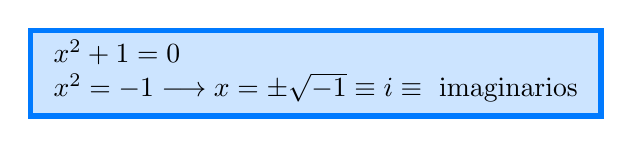
\begin{tikzpicture}
\node[draw=lightblue, fill=lightblue!20, rectangle, line
width=2pt] {$\begin{array}{l}x^2+1=0\\x^2=-1\longrightarrow
x=\pm\sqrt{-1}\equiv i\equiv~\text{imaginarios}\end{array}$};
\end{tikzpicture}

\underline{Su uso en Ciencia de Datos:} Entre otros campos se
usa en el tratamiento de señal mediante series y transformadas
de Fourier.

\begin{itemize}[leftmargin=*]
\item[\textcolor{red}{$-$}] \textcolor{lightblue}{Definición}\end{itemize}
Se llama número complejo a todo par ordenador de números reales,
$z=(x,y)$, con $x,y\in\mathbb{R}$. Por tanto, el conjunto de
todos los números complejos
$$\mathbb{C}=\mathbb{R}\times\mathbb{R}=\{z=(x,y),~~x,y\in\mathbb{R}\}$$

\begin{tikzpicture}
\draw[-latex] (-1, 0) -- (5, 0) node[right] {$x\equiv$ Eje real};\draw[-latex] (0, -1) -- (0, 5) node[above] {$y\equiv$ Eje real};\draw[->, lightblue, line
width=1.5pt] (0, 0) -- (2, 2)
node[right] {$(x,y)$};
\draw[lightblue, dashed] (2,2) -- (0,2) node[left] {parte
imaginaria$=y$};
\draw[lightblue, dashed] (2,2) -- (2,0) node[below] {parte
real$=x$};
\end{tikzpicture}

En $\mathbb{C}$ tenemos definidas dos operaciones:
\begin{enumerate}
    \item[a)] Suma: $z_1=(x_1,y_1),~z_2=(x_2,y_2)\in\mathbb{C}$

\textcolor{lightblue}{$z_1+z_2=(x_1+x_2,~y_1+y_2)\in\mathbb{C}$}
\item[b)]  Producto: $z_1=(x_1,y_1),~z_2=(x_2,y_2)\in\mathbb{C}$
\textcolor{lightblue}{$z_1\cdot z_2=(x_1\cdot x_2-y_1\cdot
y_2,~~ x_1\cdot y_2+y_1\cdot x_2)\in\mathbb{C}$}
\end{enumerate}

$\begin{array}{ll}
        \text{Ejemplo:} & z_1=(0,1)     \\
                        & z_2=(0,1)=z_1
\end{array}$\hspace{2cm}\begin{tikzpicture}[baseline=(current
bounding box.center)]
    \draw[-latex] (-2, 0) -- (3, 0) ;
    \draw[-latex] (0, -1) -- (0, 2) ;
    \fill[lightblue] (-1,0) circle (2pt) node[below] {$z_2$};
    \fill[lightblue] (0,1) circle (2pt) node[right] {$z_1$};
\end{tikzpicture}

$z_1^2=z_1\cdot z_2=(0,1)\cdot(0,1)=(0\cdot0-1\cdot1,
0\cdot1+1\cdot0)=(-1,0)$

$z_1^2=-1\rightarrow
z_1=\sqrt{-1}=i=j=(0,1)$\textcolor{lightblue}{$\longrightarrow$
unidad imaginaria pura}

\textcolor{lightblue}{\underline{Algunos números complejos
destacados}}

\begin{tikzpicture}
    \draw[-latex] (-1, 0) -- (3, 0) node[right] {eje real};
    \draw[-latex] (0, -1) -- (0, 2) node[above] {eje imaginario};
\fill[lightblue] (0,1) circle (2pt) node[right] {$j=(0,1)$};\end{tikzpicture}

$j=(0,1)=$ unidad imaginaria pura

$\{(x,0):~x\in\mathbb{R}\}$ los identificadores con los números
reales $(x,0)\equiv x$.

$\{(0,y):~y\in\mathbb{R}\}$ imaginarios puros.

\underline{Vamos a calcular:}

$\textcolor{lightblue}{\underbrace{\textcolor{black}{(x,0)}}_{x}}+\textcolor{lightblue}{\underbrace{\textcolor{black}{(0,1)}}_{\jmath}}\cdot\textcolor{lightblue}{\underbrace{\textcolor{black}{(0,y)}}_{y}}=(x,0)+(0\cdot
y-1\cdot0, ~0\cdot0+1\cdot y)=(x,0)+(0,y)=(x,y)$

$\begin{array}{l}
        x\equiv\text{ parte real} \\
y\equiv\text{ parte imaginaria. Si }z=x+\jmath \cdot
y\left\{\begin{array}{l}x=\text{Re}z\\
y=\text{Im}z\end{array}\right.
\end{array}$\hspace{2cm}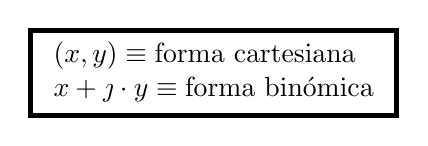
\begin{tikzpicture}[baseline=(current
bounding box.center)]
\node[draw=black, rectangle, line width=2pt]
{$\begin{array}{l}(x,y)\equiv\text{forma cartesiana}\\ x+\jmath \cdot
y\equiv\text{forma binómica}\end{array}$};
\end{tikzpicture}

\textcolor{lightblue}{\underline{Las operaciones suma y producto
en forma binómica}}

$\textcolor{lightblue}{\underbrace{\textcolor{black}{(x_1+\jmath \cdot
y_1)}}_{(x_1,~j_1)}}+\textcolor{lightblue}{\underbrace{\textcolor{black}{(x_2+\jmath \cdot
y_2)}}_{(x_2,~j_2)}}=(x_1+x_2)+\jmath \cdot(y_1+y_2)=
(x_1+x_2,~y_1+y_2)$

$\textcolor{lightblue}{\underbrace{\textcolor{black}{(x_1+\jmath \cdot
y_1)}}_{(x_1,~j_1)}}\cdot\textcolor{lightblue}{\underbrace{\textcolor{black}{(x_2+\jmath \cdot
y_2)}}_{(x_2,~j_2)}}=\begin{array}{l}
        \\
(x_1\cdot x_2-y_1\cdot y_2)+\jmath \cdot(x_1\cdot y_2+y_1\cdot x_2) \\\nwarrow j^2=-1                                               \\    \end{array}$

\newpage

\begin{wrapfigure}{r}{0.4\textwidth}
    \begin{tikzpicture}[baseline=(current bounding box.center)]
        \draw[-latex] (-2, 0) -- (4, 0) ;
        \draw[-latex] (0, -3) -- (0, 3) ;
\draw[lightblue, dashed] (0,2) -- (2,2) -- (2,-2) -- (0, -2);\draw[lightblue] (0,0) -- (2,2) node[right] {$z=x+\jmath \cdot y$};\draw[lightblue] (0,0) -- (2,-2)
node[right]
{$\overline{z}=x-\jmath \cdot y$};
        \fill[lightblue] (2,2) circle (2pt);
        \fill[lightblue] (2,-2) circle (2pt);
        \node[lightblue] at (-0.2, 2) {$y$};
        \node[lightblue] at (-0.3, -2) {$-y$};
    \end{tikzpicture}
\end{wrapfigure}

\textcolor{lightblue}{\underline{Definición (conjugado)}}

Dado $z=x+\jmath \cdot y$, se llama conjugado de $z$, denotado
$\overline{z}$, al número complejo \[\overline{z}=x-\jmath \cdot y\]

\begin{itemize}[label=\color{red}\textbullet, leftmargin=*]
    \item \textcolor{lightblue}{Propiedades del conjugado}
        \begin{enumerate}[label=\alph*)]
\item $\overline{~\overline{z}~}=z~~~~\forall z\in\mathbb{C}$\item $\overline{z+w}=\overline{z}+\overline{w}~~~~\forall
z,w\in\mathbb{C}$
\item $\overline{z\cdot
w}=\overline{z}\cdot\overline{w}~~~~\forall z,w\in\mathbb{C}$
\item $z\cdot\overline{z}=(\text{Re}z)^2+(\text{Im}z)^2$        \end{enumerate}
\end{itemize}
Veamos, por ejemplo, la última de estas propiedades $$z=x+\jmath \cdot
y,~\overline{z}=x-\jmath \cdot y\longrightarrow
z\cdot\overline{z}=(x+\jmath \cdot y)\cdot(x-\jmath \cdot
y)=x^2-\jmath  xy+\jmath  xy+y^2=x^2+y^2$$

\textcolor{lightblue}{\underline{Definición (Inverso)}}

Dado $z\in\mathbb{C}, z\neq0$, se llama inverso de $z$, denotado
$z^{-1}$ ó ${1\over z}$, al número complejo
$z^{-1}=\frac{1}{z\cdot\overline{z}}\cdot z$

Vamos a calcular $z\cdot z^{-1}$:

\textcolor{lightblue}{$z\cdot
z^{-1}=z^{-1}=\frac{1}{z\cdot\overline{z}}\cdot z\cdot
\overline{z}=\frac{\text{Re}z^2+\text{Im}z^2}{\text{Re}z^2+\text{Im}z^2}=1$}

\textcolor{lightblue}{\underline{Forma exponencial y polar de un
número complejo}}

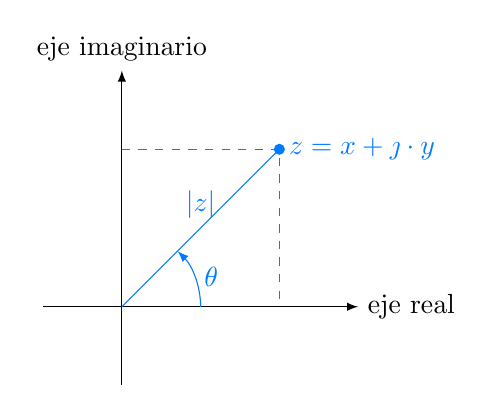
\begin{tikzpicture}
    \draw[-latex] (-1, 0) -- (3, 0) node[right] {eje real};
    \draw[-latex] (0, -1) -- (0, 3) node[above] {eje imaginario};
\draw[-latex, lightblue] (1, 0) arc (0:45:1) node[midway, right]
{$\theta$};
\draw[lightblue] (0, 0) -- (2, 2) node[midway, above] {$|z|$};    \draw[lightblue, dashed] (0, 2) -- (2, 2) -- (2,0);
\fill[lightblue] (2,2) circle (2pt) node[right] {$z=x+\jmath \cdot
y$};
\end{tikzpicture}
\begin{itemize}
\item Se llama módulo de $z$, denotado $|z|$, al número real.
          $|z|=+\sqrt{x^2+y^2}=+\sqrt{z\cdot\overline{z}}$

\item Dado $z\in\mathbb{C}, z\neq0$, se define el argumento de
$z$, denotado $\arg z$, como el conjunto

\textcolor{lightblue}{$\arg
z=\left\{\theta\in\mathbb{R}:\text{Re}z=|z|\cos\theta,~~\text{Im}z=|z|\sin\theta\right\}$}
\end{itemize}
Si $\theta\in\arg z$, entonces $\theta +2k\pi\in\arg z\forall
k\in\mathbb{Z}$.

Al único $\theta\in\arg z$ tal que $\theta\in[0,2\pi[$ se le
llama \textcolor{lightblue}{argumento principal de $z$}.

Por tanto,
$$z=\text{Re}z+\jmath \cdot\text{Im}z=|z|\cos\theta+\jmath \cdot|z|\sin\theta=|z|(\cos\theta+\jmath \cdot\sin\theta)=|z|e^{\jmath\theta}$$
donde
\textcolor{lightblue}{$e^{\jmath\theta}=\cos\theta+\jmath \cdot\sin\theta$}

En resumen, podemos expresar $z=\text{Re}z+\jmath \cdot\text{Im}z$
como:
\begin{enumerate}[label=\alph*)]
\item Forma polar
$z=|z|_\theta.~~\textcolor{lightblue}{\begin{array}{l}|z|=\text{
módulo}\\ \theta =\text{ argumento principal}\end{array}}$
    \item Forma exponencial $z=|z|\cdot e^{\jmath\theta}$
\item Forma trigonométrica
$z=|z|\cdot(\cos\theta+\jmath \cdot\sin\theta)$
\end{enumerate}
Las fornas exponencial y polar están especialmente diseñadas
para realizar las operaciones producto y cociente de números
complejos.

En efecto: $$z_1\cdot z_2=|z_1|\cdot
e^{\jmath\theta_1}\cdot|z_2|\cdot
e^{\jmath\theta_2}=|z_1|\cdot|z_2|e^{j(\theta_1+\theta_2)}=|z_1|_{\theta_1}\cdot|z_2|\cdot_{\theta_2}=|z_1|~|z_2|_{\theta_1+\theta_2}$$
es decir, se multiplican los módulos y se suman los argumentos.

La división o cociente de números complejos es multiplicar por
el inverso. Nótese que si $|z|\cdot e^{\jmath\theta}$, entonces
\[z^{-1}=\frac{1}{|z|}e^{-\jmath \theta}\text{. En efecto: }z\cdot
z^{-1}=|z|e^{\jmath\theta}=\frac{|z|}{|z|}e^{j(\theta-\theta)}=1\]

Por tanto,
\[\frac{z_1}{z_2}=\frac{|z_1|e^{\jmath\theta_1}}{|z_2|e^{\jmath\theta_2}}=\frac{|z_1|}{|z_2|}e^{j(\theta_1-\theta_2)},\]
es decir, se dividen los módulos y se restan los argumentos.

\textcolor{lightblue}{\underline{Interpretación geométrica de la
suma y el producto de números complejos}}
\begin{itemize}[label=\color{red}\textbullet]
    \item \textcolor{lightblue}{Suma (Forma binómica)}
\end{itemize}

$\left.\begin{array}{l}
        z_1=\text{Re}z_1+\jmath \cdot\text{Im}z_1 \\
        z_2=\text{Re}z_2+\jmath \cdot\text{Im}z_2
\end{array}\right\}z_1+z_2=(\text{Re}z_1+\text{Re}z_2)+\jmath \cdot(\text{Im}z_1+\text{Im}z_2)$

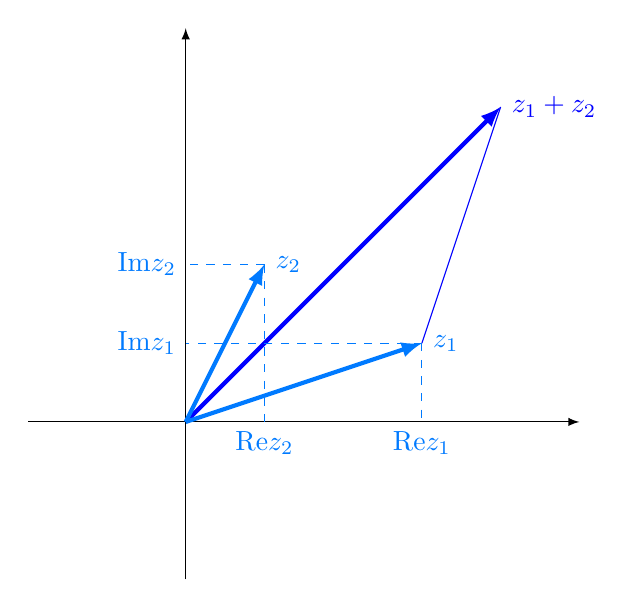
\begin{tikzpicture}
    \draw[-latex] (-2, 0) -- (5,0);
    \draw[-latex] (0,-2) -- (0,5);
\draw[-latex, blue, line width=1.5pt] (0,0) -- (4,4) node[right]
{$z_1+z_2$};
    \draw[blue] (3,1) -- (4,4);
\draw[-latex, lightblue, line width=1.5pt] (0,0) -- (3,1)
node[right] {$z_1$};
\draw[-latex, lightblue, line width=1.5pt] (0,0) -- (1,2)
node[right] {$z_2$};
\draw[lightblue, dashed] (1, 2) -- (0, 2) node[left]
{$\text{Im}z_2$};
\draw[lightblue, dashed] (3, 1) -- (0, 1) node[left]
{$\text{Im}z_1$};
\draw[lightblue, dashed] (1, 2) -- (1, 0) node[below]
{$\text{Re}z_2$};
\draw[lightblue, dashed] (3, 1) -- (3, 0) node[below]
{$\text{Re}z_1$};
\end{tikzpicture}
\begin{itemize}[label=\color{red}\textbullet]
    \item \textcolor{lightblue}{Producto}
\end{itemize}
$\left.\begin{array}{l}
        z_1=\text{Re}z_1+\jmath \cdot\text{Im}z_1 \\
        z_2=\text{Re}z_2+\jmath \cdot\text{Im}z_2
\end{array}\right\}z_1\cdot z_2=|z_1|~|z_2|_{\theta_1+\theta_2}$
\begin{tikzpicture}[baseline=(current bounding box.center)]
    \draw[-latex] (-2, 0) -- (5,0);
    \draw[-latex] (0,-2) -- (0,5);
    \draw[-latex, lightblue] (0,0) -- (4,1) node[right] {$z_1$};
    \draw[-latex, lightblue] (0,0) -- (2,1) node[right] {$z_2$};
\draw[-latex, lightblue] (0,0) -- (3,4) node[right] {$z_1\cdot
z_2$};
\draw[-latex, blue] (3,0) arc (0:53:3) node[midway,right]
{$\theta_1+ \theta_2$};
\draw[-latex, blue] (1,0) arc (0:27:1) node[midway,right]
{$\theta_2$};
\draw[-latex, blue] (2,0) arc (0:14:2) node[midway,right]
{$\theta_1$};
\end{tikzpicture}

\textcolor{lightblue}{¿Cómo pasar los números complejos de una
forma a otra?}

Binómica$\longrightarrow$ Polar/exponencial

$z=x+\jmath \cdot y\longrightarrow\left\{\begin{array}{l}
        |z|=+\sqrt{x^2+y^2} \\
        \theta=\arg z=\arctan \frac{y}{x}
    \end{array}\right.$

Las calculadoras solo devuelven valores del arcotangente en
$-90^\circ$ y $90^\circ$. Dependiendo de la localización del
número complejo en cuestión hay que sumar $180^\circ$.

\begin{tikzpicture}
    \draw[-latex] (-3, 0) -- (3,0);
    \draw[-latex] ( 0,-3) -- (0,3);
    \draw[lightblue] ( -2,2) -- (2,-2);
    \fill[lightblue] (-2,2) circle (2pt) node[left] {$z_2$};
    \fill[lightblue] (2,-2) circle (2pt) node[right] {$z_1$};
\end{tikzpicture}

$z_1$ y $z_2$ tienen el mismo arcotangente, según la
calculadora.

Veamos algunos ejemplos:
\begin{itemize}
    \item $1+\jmath \longrightarrow|1+\jmath |=+\sqrt{1^2+1^2}=\sqrt{2}$
\end{itemize}
\begin{tikzpicture}[scale=0.5, baseline=(current bounding
box.center)]
    \draw[-latex] (-3, 0) -- (3,0);
    \draw[-latex] ( 0,-3) -- (0,3);
\draw[-latex, lightblue, line width=1.5pt] (0,0) -- (2,2)
node[right] {$1+\jmath $};
    \draw[dashed, lightblue, thick] (0,2) -- (2,2) -- (2,0);
\end{tikzpicture}
$\begin{array}{l}
\theta=\arctan \frac{1}{1} =45^\circ=\frac{\pi}{4} \text{
radianes} \\
        1+\jmath =\sqrt{2}_{45^\circ}=\sqrt{2}e^{j\frac{\pi}{4}}
    \end{array}$
\begin{itemize}
\item
$-1-\jmath \longrightarrow|-1-\jmath |=+\sqrt{(-1)^2+(-1)^2}=+\sqrt{2}$
\end{itemize}
\begin{tikzpicture}[scale=0.5, baseline=(current bounding
box.center)]
    \draw[-latex] (-3, 0) -- (3,0);
    \draw[-latex] ( 0,-3) -- (0,3);
\draw[-latex, lightblue, line width=1.5pt] (0,0) -- (-2,-2)
node[below] {$-1-\jmath $};
\draw[dashed, lightblue, thick] (0,-2) -- (-2,-2) -- (-2,0);\end{tikzpicture}
$\begin{array}{l}
\theta=\arctan \frac{-1}{-1}
=45^\circ=45^\circ+180^\circ=225^\circ=\frac{\pi}{4}+\pi=\frac{5\pi}{4}\text{
rad.} \\
        -1-\jmath =\sqrt{2}_{225^\circ}=+\sqrt{2}e^{j\frac{5\pi}{4}}
    \end{array}$

Polar|Exponencial$\longrightarrow$Binómica

$z=|z|_\theta=|z|e^{\jmath\theta}\longrightarrow
z=|z|(\cos\theta+\jmath \cdot\sin\theta)=|z|\cos\theta+\jmath |z|\sin\theta$

\textcolor{lightblue}{\underline{Ejemplos}}

\begin{multicols}{2}
    \begin{itemize}
        \item $1\pi=1\cdot e^{\jmath\pi}=\cos\pi+\jmath \cdot\sin\pi=-1$
    \end{itemize}
    \begin{tikzpicture}
        \draw[-latex] (-2, 0) -- (2,0);
        \draw[-latex] (0, -1) -- (0,2);
\draw[lightblue] (-1, 0.1) -- (-1,-0.1) node[below] {$1\pi$};    \end{tikzpicture}
    \columnbreak
    \begin{itemize}
\item $2_{\frac{\pi}{3}}=2\cdot
e^{j\frac{\pi}{3}}=2(\cos\frac{\pi}{3}+\jmath \cdot\sin\frac{\pi}{3})=2\cdot(0.5+\jmath \cdot0.866)=1+\jmath \cdot1.732$
    \end{itemize}
    \begin{tikzpicture}
        \draw[-latex] (-2, 0) -- (2,0);
        \draw[-latex] (0, -1) -- (0,2);
\draw[lightblue] (0,0) -- (pi/3,1) node[right] {$\pi\over 3$};        \draw[-latex, lightblue] (0.8,0) arc (0:44:0.8);
\draw[lightblue, dashed] (0,1) -- (pi/3, 1) -- (pi/3, 0);        \fill[lightblue] (pi/3,1) circle (2pt) ;
    \end{tikzpicture}
\end{multicols}
\textcolor{lightblue}{\underline{Un ejemplo de uso de los
números complejos en Ciencia de Datos}}

En algunos campos de la Ciencia de Datos y la Inteligencia
Artificial, e.g. reconocimiento del hablante o asistentes
virtuales (Siri, en Apple), es necesario analizar y procesar
señales, las cuales desde los tiempos de Fourier (siglo XIX), se
procesan mediante una superposición de funciones trigonométricas
con frecuencia discreta (series de Fourier) o continua
(transformada de Fourier). En concreto, las señales periódicas
se representan mediante series de Fourier y las no periódicas
mediante transformadas de Fourier. Como veremos a continuación,
los dos parámetros fundamentales de una onda son su frecuencia.
Esto nos recuerda al módulo y argumento de un número complejo.
Efectivamente, esto es así y es precisamente la forma
exponencial de los números complejos la que facilita el
procesamiento de estas señales.

Antes de nada, conviene señalar la conexión entre las funciones
trigonométricas seno y coseno, y las exponenciales complejas.

Se tiene:

$\cos\theta=\frac{e^{\jmath\theta}+e^{-\jmath \theta}}{2}$

En efecto:

$e^{\jmath\theta}=\cos\theta+\jmath \cdot\sin\theta$

$e^{-\jmath \theta}=\cos(-\theta)+\jmath \cdot\sin(-\theta)=\cos\theta-\jmath \cdot\sin\theta$

Por tanto:$$e^{\jmath\theta}+e^{-\jmath \theta}=2\cos\theta$$

De igual forma, $\sin\theta=\frac{e^{\jmath\theta}-e^{-\jmath \theta}}{2\jmath}$
\textcolor{lightblue}{\underline{Representación matemática de
una honda elemental}}
\begin{itemize}
\item La función $\cos
t=\frac{e^{jt}+e^{-\jmath  t}}{2},~t\equiv$tiempo.
\end{itemize}
\begin{tikzpicture}
    \draw[-latex] (-2,0)--(9,0);
    \draw[-latex] (0,-2)--(0,2);
    \draw[dashed] (-2,1)--(9,1);
    \draw[dashed] (-2,-1)--(9,-1);

\draw[domain=2*pi:9, variable=\x, lightblue, dashed] plot
({\x},{cos(\x r)});
\draw[domain=-2:0, variable=\x, lightblue, dashed] plot
({\x},{cos(\x r)});
\draw[domain=0:2*pi, variable=\x, lightblue] plot ({\x},{cos(\x
r)});
    \foreach \y in {-1, 1}
    \draw (0.1, \y) -- (-0.1, \y) node[left] {$\y$};
\draw[lightblue] (pi/2, 0.1) -- (pi/2,-0.1) node[below]
{$\pi\over2$};
\draw[lightblue] (pi, 0.1) -- (pi,-0.1) node[below] {$\pi$};\draw[lightblue] (3*pi/2, 0.1) -- (3*pi/2,-0.1) node[below]
{$3\pi\over2$};
\draw[lightblue] (2*pi, 0.1) -- (2*pi,-0.1) node[below]
{$2\pi$};
\node[draw=black, rectangle, line width=1pt] at (12, 0)
{Periodo\hspace{0.3cm}$T=2\pi$};
\end{tikzpicture}
\begin{itemize}
    \item La función $A\cos t=\frac{Ae^{jt}+Ae^{-\jmath  t}}{2}$
\end{itemize}
\begin{tikzpicture}
    \draw[-latex] (-2,0)--(7,0) node[right] {$t$};
    \draw[-latex] (0,-2)--(0,2);
    \draw[dashed] (0,1)--(7,1);
    \draw[dashed] (0,-1)--(7,-1);

\draw[domain=0:2*pi, variable=\x, lightblue] plot ({\x},{cos(\x
r)});
\draw[lightblue] (pi/2, 0.1) -- (pi/2,-0.1) node[below]
{$\pi\over2$};
\draw[lightblue] (pi, 0.1) -- (pi,-0.1) node[below] {$\pi$};\draw[lightblue] (3*pi/2, 0.1) -- (3*pi/2,-0.1) node[below]
{$3\pi\over2$};
\draw[lightblue] (2*pi, 0.1) -- (2*pi,-0.1) node[below]
{$2\pi$};
    \draw (0.1, 1) -- (-0.1, 1) node[left] {$A$};
    \draw (0.1, -1) -- (-0.1, -1) node[left] {$-A$};
\node[draw=black, rectangle, line width=1pt] at (12, 0)
{Periodo\hspace{0.3cm}$A\equiv$ Amplitud de la onda};
\end{tikzpicture}

\begin{itemize}
    \item La función $\cos(wt)=\frac{e^{jwt}+e^{-\jmath wt}}{2}$
\end{itemize}
Periodo de $T$ es tal que $wT=2\pi\longrightarrow
T=\frac{2\pi}{w}$

Si $w$ es pequeño$\longrightarrow ~T$ es grande (pocas
oscilaciones)

\begin{tikzpicture}
    \draw[-latex] (-2,0)--(7,0) node[right] {$t$};
    \draw[-latex] (0,-2)--(0,2);

\draw[domain=0:2*pi, variable=\x, lightblue] plot ({\x},{cos(\x
r)});

    \foreach \y in {-1, 1}
    \draw (0.1, \y) -- (-0.1, \y) node[left] {$\y$};
\draw[lightblue] (2*pi, 0.1) -- (2*pi,-0.1) node[below] {$T$};\end{tikzpicture}

Si $w$ es grande$\longrightarrow ~T$ es pequeño (muchas
oscilaciones)

\begin{tikzpicture}
    \draw[-latex] (-2,0)--(7,0) node[right] {$t$};
    \draw[-latex] (0,-2)--(0,2);

\draw[domain=0:pi, variable=\x, lightblue] plot ({\x},{cos(2*\x
r)});
\draw[domain=pi:2*pi, variable=\x, lightblue, dashed] plot
({\x},{cos(2*\x r)});

    \foreach \y in {-1, 1}
    \draw (0.1, \y) -- (-0.1, \y) node[left] {$\y$};
    \draw[lightblue] (pi, 0.1) -- (pi,-0.1) node[below] {$T$};
\end{tikzpicture}

frecuencia $f=\frac{1}{T}=\frac{w}{2\pi}$

velocidad angular $\frac{2pi}{T}=w$

\begin{itemize}
\item La función $\cos
(t-\varphi)=\frac{e^{j(t-\varphi)}+e^{-\jmath (t-\varphi)}}{2}$
\end{itemize}
\begin{tikzpicture}
    \draw[-latex] (-2,0)--(7,0) node[right] {$t$};
    \draw[-latex] (0,-2)--(0,2);
    \draw[dashed] (0,1)--(7,1);
    \draw[dashed] (0,-1)--(7,-1);
    \draw[dashed] (0.5,1)--(0.5,0) node[below] {$\varphi$};

\draw[domain=0:2*pi, variable=\x, lightblue] plot ({\x},{cos(\x
r)});

    \foreach \y in {-1, 1}
    \draw (0.1, \y) -- (-0.1, \y) node[left] {$\y$};
\end{tikzpicture}

Si $t=\varphi\longrightarrow\cos(t-\varphi)=\cos0=1$

$\varphi\equiv$ fase inicial

$\varphi$ traslada la honda hacia la derecha
\textcolor{red}{($\varphi$ positiva)} o hacia la izquierda
\textcolor{lightblue}{($\varphi$ negativa)}.

\textcolor{lightblue}{\underline{En resumen}}

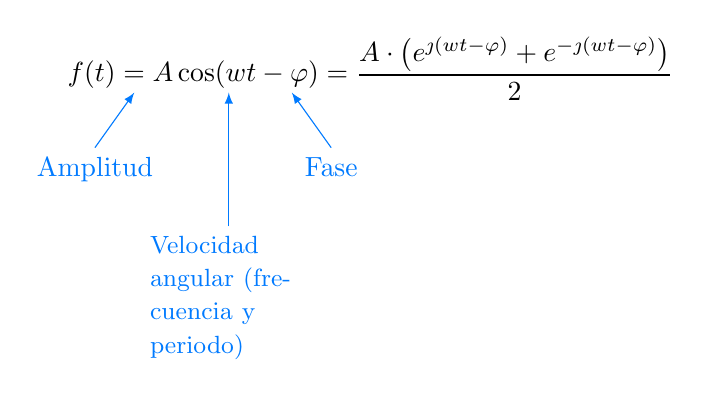
\begin{tikzpicture}
\node at (0,0)
{$f(t)=A\cos(wt-\varphi)=\dfrac{A\cdot\left(e^{\jmath(wt-\varphi)}+e^{-\jmath (wt-\varphi)}\right)}{2}$};
\draw[lightblue, -latex] (-3.5,-1) node[below] {Amplitud} --
(-3,-0.3);
\draw[lightblue, -latex] (-1.8,-2) node[below, text width=2cm]
{\small Velocidad angular (frecuencia y periodo)} --
(-1.8,-0.3);
\draw[lightblue, -latex] (-0.5,-1) node[below] {Fase} --
(-1,-0.3);
\end{tikzpicture}

\textcolor{lightblue}{\underline{Raices $n$-ésimas y raices de
polinomios}}

Consideremos la ecuación $x^2+1=0$.

Como sabemos, no existe ningún número real que sea solución de
dicha ecuación.

Veamos si hay algún número complejo.

Buscamos $z=|z|e^{\jmath\theta}$ tal que

\hspace{2cm}$z^2=|z|^2e^{2\jmath\theta}=-1=e^{\jmath\pi}$.

\begin{wrapfigure}{r}{0.3\textwidth}
    
\begin{tikzpicture}[scale=0.7]
        \draw (-2.5,0) -- (2.5,0);
        \draw (0,-2.5) -- (0,2.5);
        \draw[lightblue, line width=1.5pt] (0,0) circle (2);
    \end{tikzpicture}
\end{wrapfigure}

Para que dos números complejos sean iguales sus módulos han de
ser iguales y sus argumentos diferir en un múltiplo de $2\pi$.
Por tanto:

$\left.\begin{array}{r}
        |z|^2=1 \\
        2\theta=\pi+2k\pi
    \end{array}\right\}~~~~\begin{array}{l}
        |z|=+\sqrt{1}=1 \\
        \theta=\dfrac{\pi}{2}+k\pi
    \end{array}$

$k=0\longrightarrow\theta_1=\dfrac{\pi}{2}$

$k=1\longrightarrow\theta_2=\dfrac{\pi}{2}+\pi=\dfrac{3\pi}{2}$

$k=2\longrightarrow\theta_3=\dfrac{\pi}{2}+3\pi=\dfrac{7\pi}{2}=(\text{Como
argumentos})=\dfrac{3\pi}{2}$

$k=-1\longrightarrow\theta_4=\dfrac{\pi}{2}-\pi=-\dfrac{\pi}{2}=(\text{Como
argumentos})=\dfrac{3\pi}{2}$

\begin{tikzpicture}
    \draw (7.5,0) -- (12.5,0);
    \draw (10,-2.5) -- (10,2.5);
    \draw[lightblue] (10,0) circle (2);
    \fill[blue] (10,2) circle (3pt) node[above] {$~~~~z_1$};
    \fill[blue] (10,-2) circle (3pt) node[below] {$~~~~z_2$};
\node[text width=12cm] at (0,0) {Por tanto, la ecuación
$x^2+1=0$ tiene dos soluciones en\\
        $\mathbb{C}:\left\{\begin{array}{l}
                z_1=e^{j\frac{\pi}{2}} \\
                z_2=e^{j\frac{3\pi}{2}}
            \end{array}\right.$};
\end{tikzpicture}

Veamos que los argumentos se van repartiendo.

Solo hay dos argumentos en $\left[0,2\pi\right[$.

Se las llamas \textcolor{lightblue}{"raíces cuadráticas de la
unidad"}.

Para la ecuación $x^3+1=0$ procedemos de igual modo: buscamos
$z=|z|e^{\jmath\theta}$ tal que $z^3=|z|^3e^{3\jmath\theta}=-1=e^{\jmath\pi}$.

\begin{wrapfigure}{r}{0.3\textwidth}
    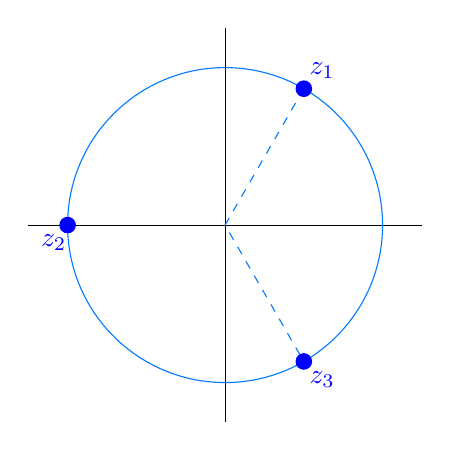
\begin{tikzpicture}
        \draw (-2.5,0) -- (2.5,0);
        \draw (0,-2.5) -- (0,2.5);
        \draw[lightblue] (0,0) circle (2);
\draw[lightblue, dashed] (60:2) -- (0,0) -- (300:2);
\fill[blue] (60:2) circle (3pt) node[above] {$~~~~z_1$};
\fill[blue] (300:2) circle
(3pt) node[below] {$~~~~z_3$};
\fill[blue] (-2,0) circle (3pt) node[below] {$z_2$~~~~}; 
\end{tikzpicture}
\end{wrapfigure}

Por tanto:

$|z|^3=1\longrightarrow|z|=1$

$3\theta=\pi+2k\pi\longrightarrow\theta=\dfrac{\pi}{3}+\dfrac{2k\pi}{3}$

$k=0\longrightarrow\theta_1=\dfrac{\pi}{3}$

$k=1\longrightarrow\theta_2=\dfrac{\pi}{3}+\dfrac{2\pi}{3}$

$k=2\longrightarrow\theta_3=\dfrac{\pi}{3}+\dfrac{4\pi}{3}$

Las raíces cúbicas de la unidad son $\left\lbrace
e^{j\frac{\pi}{3}},e^{\jmath\pi},e^{j\left(\frac{\pi}{3}+\frac{4\pi}{3}\right)}\right\rbrace$

En general, la ecuación $x^n+1=0$ tiene n-raíces en
$\mathbb{C}$, llamadas raíces $n$-ésimas de la unidad y son:
\[\left\{z=|z|e^{\jmath\theta}:|z|=1=\dfrac{\pi}{n}+\dfrac{2k\pi}{n},k=0,1,\hdots,n-1\right\}\]

Para completar, se puede demostrar (lo hizo Gauss en su tesis
doctoral) que todo polinomio de grado $n$ tiene directamente
n-raíces (reales y/o complejas). Es el llamado Teorema
Fundamental del Álgebra.

\newpage

\section{Espacios vectoriales de dimensión finita}
\textcolor{lightblue}{\underline{Vectores}}

Sea $\mathbb{K}=\mathbb{R}$ ó $\mathbb{C}$. A los elementos de
$\mathbb{K}$ les llamamos \textcolor{lightblue}{escalares}.
\begin{itemize}[label=\color{red}\textbullet, leftmargin=*]
\item \color{lightblue} Definición (Espacio vectorial de
dimensión finita)
\end{itemize}
Sea $n\in\mathbb{N}$. Definimos
\[\mathbb{K}^n=\{(x_1,x_2,\hdots,x_n)\}:x_i\in\mathbb{K},1\le
i\le n\]
A los elementos $v=(x_1,\hdots,x_n)\in\mathbb{K}^n$ se les llama
vectores de componentes en $\mathbb{K}$.

En Python se les llaman 1d-array.

En $\mathbb{K}^n$ tenemos definidas dos operaciones:
\begin{itemize}
    \item Suma de vectores:

\fcolorbox{lightblue}{lightblue!10}{$u+v=(x_1,x_2,\hdots,x_n)+(y_1,y_2,\hdots,y_n)=(x_1+y_1,x_2+y_2,\hdots,x_n+y_n)$}

\item Producto por escalares: $\lambda\in\mathbb{K}$,
$u\in\mathbb{K}^n$

\fcolorbox{lightblue}{lightblue!10}{$\lambda\cdot
u=\lambda\cdot(x_1,\hdots,x_n)=(\lambda x_1,\lambda
x_2,\hdots,\lambda x_n)\in\mathbb{K}^n$}
\end{itemize}
Al conjunto de vectores $\mathbb{K}^n$ con las dos operaciones
anteriores se le llama \textcolor{lightblue}{espacio vectorial
sobre $\mathbb{K}$.}

\textcolor{lightblue}{\underline{Dependencia lineal}}
\begin{itemize}[label=\color{red}\textbullet, leftmargin=*]
    \item \color{lightblue}Definición (Combinación lineal)
\end{itemize}
Dados vectores $u,u_1,u_2,\hdots,u_m\in\mathbb{K}^n$, se dice
que $u$ es \textcolor{lightblue}{combinación lineal} de
$u_1,u_2,\hdots,u_n$ si existen escalares
$\lambda_1,\lambda_2,\hdots,\lambda_m\in\mathbb{K}^n$ de modo
que $u$ puede expresarse como
\begin{center}
\fcolorbox{lightblue}{lightblue!10}{$\lambda_1u_1+\lambda_2u_2+\cdots+\lambda_mu_m=0=(0,\hdots,0)$}
\end{center}
se cumple que $\lambda_1=\lambda_2=\cdots=\lambda_m=0$.

Es decir, la única forma de obtener una combinación lineal nula
es como todos los coeficientes nulos.
\begin{itemize}[label=\color{red}\textbullet]
    \item \textcolor{lightblue}{Demostración}
\end{itemize}
\begin{itemize}[label=$\longrightarrow$]
\item Supongamos que $\{u_1,u_2,\hdots,u_m\}$ es linealmente
independiente y que

\fcolorbox{lightblue}{lightblue!10}{$\lambda_1 u_1+\lambda_2
u_2+\cdots+\lambda_mu_m=0$}

Si algún $\lambda_i$ fuese nulo, por ejemplo $\lambda_1\neq0$,
entonces

\fcolorbox{lightblue}{lightblue!10}{$u_1=\dfrac{\lambda_2}{\lambda_1}u_2+\cdots+\dfrac{\lambda_m}{\lambda_1}u_m$}

          y así $u_1$ es combinación lineal de los demás.

    \item Recíprocamente, supongamos que si

\fcolorbox{lightblue}{lightblue!10}{$\lambda_1u_1+\lambda_2u_2+\cdots+\lambda_mu_m=0$}

          entonces $\lambda_1=\lambda_2=\cdots=\lambda_m=0$

El conjunto $\{u_1,u_2,\hdots,u_m\}$ ha de ser linealmente
independiente pues si no lo fuera entonces al giro de sus
vectores, por ejemplo $u_2$, se podría expresar

\fcolorbox{lightblue}{lightblue!10}{$u_1=\lambda_2u_2+\cdots+\lambda_mu_m$}

          y entonces

\fcolorbox{lightblue}{lightblue!10}{$u_1-\lambda_2u_2-\cdots-\lambda_mu_m=0$}

sería una combinación lineal nula con al menos un coeficiente,
el 1 que acompaña a $u_1$, no nulo.
\end{itemize}
\begin{itemize}[label=\color{red}\textbullet, leftmargin=*]
\item \color{lightblue} Definición (Rotación de dependencia)\end{itemize}
Dados unos vectores $u_1,u_2,\hdots,u_m$ linealmente
dependientes, se llama \textcolor{lightblue}{relación de
dependencia} a cualquier combinación lineal nula
\[\lambda_1u_1,\lambda_2 u_2,\hdots,\lambda_mu_m=0\] con no
todos los coeficientes nulos.
\begin{itemize}[label=\color{red}\textbullet, leftmargin=*]
    \item \color{lightblue} Definición (Base canónica)
\end{itemize}
El conjunto de vectores \begin{center}
\fcolorbox{lightblue}{lightblue!10}{$C=\{e_1=(1,0,0,\hdots,0),e_2=(0,1,0,\hdots,0),\hdots,e_n=(0,0,\hdots,0,1)\subset\mathbb{K}^n\}$}
\end{center} se llama \textcolor{lightblue}{base canónica} de
$\mathbb{K}^n$.

Se trata de un conjunto de vectores linealmente independiente y
cada vector $u=(a_1,a_2,\hdots,a_n)\in\mathbb{K}^n$ se escribe
como combinación lineal en $C$ en la forma

\fcolorbox{lightblue}{lightblue!10}{$u=a_1e_1+a_2e_2+\cdots+a_ne_n$}
\begin{itemize}[label=\color{red}\textbullet, leftmargin=*]
    \item \color{lightblue} Proposición
\end{itemize}
Sean $S=\{u_1,u_2,\hdots,u_m\}$ un conjunto de vectores
linealmente independientes y $u\in\mathbb{K}^n$. Entonces:
\begin{enumerate}
\item Todo subconjunto de $S$ no vacía es linealmente
independiente.
\item El conjunto $S\cap\{u\}$ es linealmente independiente si y
sólo si $u$ no es combinación lineal de $u_1,u_2,\hdots,u_m$.
\end{enumerate}
\textcolor{lightblue}{\underline{Norma y producto escalar}}
\begin{itemize}[label=\color{red}\textbullet, leftmargin=*]
    \item \color{lightblue} Definición (Norma euclídea)
\end{itemize}
Sea $u=(x_1,x_2,\hdots,x_n)\in\mathbb{R}^n$. Se llama norma
euclídea o norma 2, escalar.
\begin{center}
\fcolorbox{lightblue}{lightblue!10}{$\|u\|_2=+\sqrt{x_1^2+\cdots+x_n^2}$}
\end{center}
Si $\|u\|_2=1$, $u$ se dice unitario.

Otras normas utilizadas en Ciencia de Datos son:

$\|u\|_1=|x_1|+|x_2|+\cdots+|x_n|=\sum_{j=1}^{n}|x_j|$

$\|u\|_p=\left(|u_1|^p+|u_2|^p+\cdots+|u_n|^p\right)^{\frac{1}{p}}$,
$1<p<+\infty$

$\|u\|_{\infty}=\max\{|x_1|+|x_2|+\cdots+|x_n|\}~~1\le j\le
n\longrightarrow$ Norma del máximo o norma del infinito.

\begin{itemize}[label=\color{red}\textbullet, leftmargin=*]
    \item \color{lightblue} Ejemplo
\end{itemize}

$u=(1,-2,-1)$

$\|u\|_1=|1|+|-2|+|-1|=4$

$\|u\|_2=\sqrt{1^2+(-2)^2+(-1)^2}=+\sqrt{6}$

$\|u\|_\infty=\max\{|1|,|-2|,|-1|\}=2$

Todas las normas comparten las siguientes propiedades:
\begin{itemize}
\item Sean $\|\cdot\|$ cualquiera de las normas anteriores,
$u\in\mathbb{R}^n$ y $\alpha\in\mathbb{R}$. Entonces:
          \begin{enumerate}[label=\alph*)]
              \item $\|u\|\ge0$ y $\|u\|=0$ si y sólo si $u=0$.
              \item $\|\alpha u\|=|\alpha|\cdot\|u\|$
\item $\|u+v\|\le\|u\|+\|v\|$ (desigualdad triangular)          \end{enumerate}
\item[$\longrightarrow$] A partir de ahora, salvo que se indique
lo contrario, $\|\cdot\|=\|\cdot\|_2$ la norma euclídea.
\end{itemize}

\begin{itemize}[label=\color{red}\textbullet, leftmargin=*]
\item \color{lightblue} Definición (Producto escalar euclídeo)\end{itemize}
Dados
$u=(x_1,x_2,\hdots,x_n),v=(y_1,y_2,\hdots,y_n)\in\mathbb{R}^n$,
se define el producto escalar euclídeo de $u$ por $v$ como
\[u\cdot v=x_1\cdot y_1+x_2\cdot y_2+\cdots+x_n\cdot y_n\]
Nótese que entonces $\|u\|_2=\sqrt{u\cdot u}$
\begin{itemize}[label=\color{red}\textbullet, leftmargin=*]
    \item \color{lightblue} Propiedades del producto escalar
\end{itemize}
\begin{enumerate}[label=\alph*)]
    \item $(u_1+u_2)\cdot v=u_1\cdot v+u_2\cdot v$.
    \item $u\cdot(v_1+v_2)=u\cdot v_1+u\cdot v_2$.
\item $(\alpha\cdot u)\cdot v=u\cdot(\alpha\cdot
v)=\alpha(u\cdot v)$.
    \item $u\cdot v=v\cdot u$.
    \item $u\cdot u\ge0$ y $u\cdot u=0$ si y sólo si $u=0$.
\end{enumerate}
\begin{itemize}[label=\color{red}\textbullet, leftmargin=*]
    \item \color{lightblue} Propiedades de la norma euclídea.
\end{itemize}
\begin{enumerate}
    \item $\|u+v\|^2=\|u\|^2+\|v\|^2+2(u\cdot v)$
    \item $\|u-v\|^2=\|u\|^2+\|v\|^2-2(u\cdot v)$
\item $|u\cdot v|\le\|u\|\cdot\|v\|\longrightarrow$ Desigualdad
de Cauchy-Schwarz
\end{enumerate}
\begin{itemize}[label=\color{red}\textbullet, leftmargin=*]
    \item \color{lightblue} Demostración
\end{itemize}
Veamos el punto \textcolor{lightblue}{(3)}.

Si $u=0$ los dos miembros son nulos y se cumple la desigualdad.
Supongamos $v\neq0$. Entonces:

$0\le\left(u-\frac{u\cdot
v}{\|v\|^2}v\right)\cdot\left(u-\frac{u\cdot
v}{\|v\|^2}v\right)=u\cdot\left(u-\frac{u\cdot
v}{\|v\|^2}v\right)-\frac{u\cdot v}{\|v\|^2}\cdot
v\cdot\left(u-\frac{u\cdot v}{\|v\|^2}v\right)=$

$u\cdot u-\frac{u\cdot v}{\|v\|^2}\cdot u\cdot v-\frac{u\cdot
v}{\|v\|^2}\cdot v\cdot u+\frac{u\cdot
v}{\|v\|^2}\cdot\frac{u\cdot v}{\|v\|^2}\cdot v\cdot
v=\|u\|^2-\frac{2(u\cdot v)^2}{\|v\|^2}+\frac{(u\cdot
v)^2}{\|v\|^2}=\|u\|^2-\frac{|u\cdot v|^2}{\|v\|^2}$

Nótese que como consecuencia de la desigualdad de
Cauchy-Schwarz, si $u,v$ son vectores no nulos, entonces
$-1\le\dfrac{u\cdot v}{\|u\|\cdot\|v\|}\le1$.

Por tanto, existe un único ángulo $0\le\varphi\le\pi$ tal que
$\cos\varphi=\frac{u\cdot v}{\|u\|\cdot\|v\|}$.

A este ángulo se le llama ángulo formado por los vectores $u$ y
$v$ y su coseno se denota $\cos(u,v)$. Así, $u\cdot
v=\|u\|\cdot\|v\|\cos(u,v)$.
\begin{itemize}[label=\color{red}\textbullet, leftmargin=*]
    \item \color{lightblue} Ejemplo:
\end{itemize}
\begin{tikzpicture}[scale=2.5]
    \draw[-latex] (-0.5,0) -- (1.5,0);
    \draw[-latex] (0,-0.5) -- (0,1.5);
\draw[-latex, lightblue, line width=2pt] (0,0) -- (0,1)
node[right] {$v=(0,1)$};
\draw[-latex, lightblue, line width=2pt] (0,0) -- (1,0)
node[below] {$u=(1,0)$};
    \node[text width=6cm] at (3,1) {$\begin{array}{l}
u\cdot v=(1,0)\cdot(0,1)=1\cdot0+0\cdot 1=0 \\\cos(u,v)=0\longrightarrow\varphi=90\text{º}=\frac{\pi}{2} \\\|u\|=\|v\|=1 \\ \end{array}$};
\end{tikzpicture}

$u\cdot v$ son perpendiculares (ortogonales).
\begin{itemize}[label=\color{red}\textbullet, leftmargin=*]
    \item \color{lightblue} Definición (ortogonalidad)
\end{itemize}
Dos vectores $u,v\in\mathbb{K}^n$ se llaman ortogonales o
perpendiculares si $u\cdot v=0$.

Como consecuencia $\|u\pm v\|^2=\|u\|^2+\|v\|^2$ si $u$ y $v$
son perpendiculares (Teorema de Pitágoras).

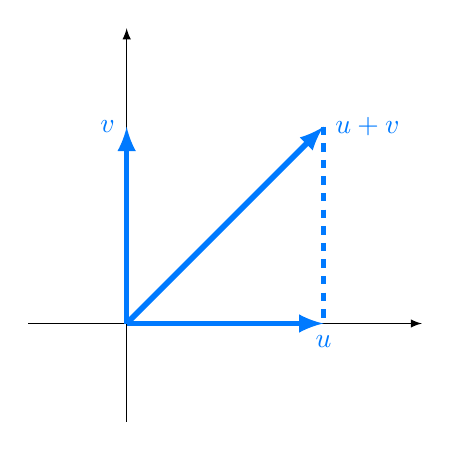
\begin{tikzpicture}[scale=2.5]
    \draw[-latex] (-0.5,0) -- (1.5,0);
    \draw[-latex] (0,-0.5) -- (0,1.5);
\draw[-latex, lightblue, line width=2pt] (0,0) -- (0,1)
node[left] {$v$};
\draw[-latex, lightblue, line width=2pt] (0,0) -- (1,0)
node[below] {$u$};
\draw[-latex, lightblue, line width=2pt] (0,0) -- (1,1)
node[right] {$u+v$};
    \draw[lightblue, dashed, line width=1.5pt] (1,1) -- (1,0);
\end{tikzpicture}
\begin{itemize}[label=\color{red}\textbullet, leftmargin=*]
    \item \color{lightblue} Definición
\end{itemize}
Un conjunto de vectores $\{u_1,\hdots,u_n\}\subset\mathbb{K}^n$
se dice \textcolor{lightblue}{ortogonal} si $u_i\cdot
u_i=0,i\neq j$. Si además los vectores son unitarios, el
conjunto se dice ortonormal.
\begin{itemize}[label=\color{red}\textbullet, leftmargin=*]
    \item \color{lightblue} Ejemplo:
\end{itemize}
La base canónica $C=\{e_1,\hdots,e_n\}$ es ortonormal.
\begin{itemize}[label=\color{red}\textbullet, leftmargin=*]
    \item \color{lightblue} Propiedades
\end{itemize}
Todo conjunto ortogonal es linealmente independiente.
\begin{itemize}[label=\color{red}\textbullet, leftmargin=*]
    \item \color{lightblue} Demostración
\end{itemize}
Sea $\{u_1,\hdots,u_m\}$ ortogonal.
$\lambda_1u_1+\lambda_2u_2+\cdots+\lambda_mu_m=0$. Multiplicando
por $u_j$:

$\lambda_1u_1u_j+\lambda_2u_2u_j+\cdots+\lambda_ju_j\cdot
u_j+\cdots+\lambda_mu_m\cdot
u_j=0\longrightarrow\lambda_j\|u_j\|^2=0\longrightarrow
\lambda_j=0$

\textcolor{lightblue}{\underline{Matrices}}

\begin{itemize}[label=\color{red}\textbullet, leftmargin=*]
\item \color{lightblue} Definición: (Matriz de tamaño $m\times
n$)
\end{itemize}
Sean $m,n\in\mathbb{N}$. Se llama matriz de tamaño $m\times n$
al conjunto formado por m-vectores de n-componentes apilados
verticalmente. En Python, a las matriz se les llama 2d-array.
\begin{itemize}[label=\color{red}\textbullet, leftmargin=*]
    \item \color{lightblue} Ejemplo (Matriz de Hilbert)
\end{itemize}
Matriz $H$ con entradas $H_{\imath\jmath  }=\dfrac{1}{i+\jmath -1}$

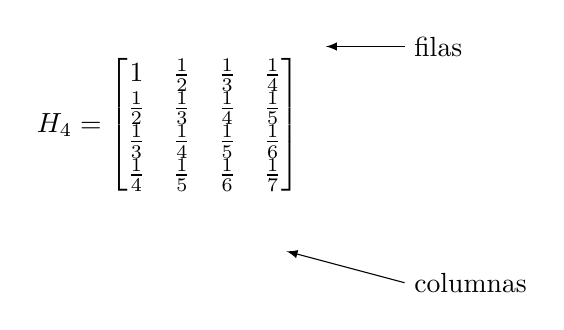
\begin{tikzpicture}
    \node at (0,0) {$H_4=\begin{bmatrix}
1 & \textstyle{\frac{1}{2}} & \textstyle{\frac{1}{3}} &
\textstyle{\frac{1}{4}} \\
\textstyle{\frac{1}{2}} & \textstyle{\frac{1}{3}} &
\textstyle{\frac{1}{4}} & \textstyle{\frac{1}{5}} \\
\textstyle{\frac{1}{3}} & \textstyle{\frac{1}{4}} &
\textstyle{\frac{1}{5}} & \textstyle{\frac{1}{6}} \\
\textstyle{\frac{1}{4}} & \textstyle{\frac{1}{5}} &
\textstyle{\frac{1}{6}} & \textstyle{\frac{1}{7}}
            \end{bmatrix}$};
    \draw[-latex] (3,1) node[right] {filas} -- (2,1);
    \draw[-latex] (3,-2) node[right] {columnas} -- (1.5, -1.6);
\end{tikzpicture}

Denotaremos por $M_{m\times n}(\mathbb{K})$ al conjunto de
matrices de m-filas y n-columnas con entradas en
$\mathbb{K}=\mathbb{R}$ ó $\mathbb{C}$.

Si $m=n$, es decir, la matriz cuadrada (tiene el mismo número de
filas que de columnas), entonces escribimos $M_n(\mathbb{K})$.

\begin{itemize}[label=\color{red}\textbullet, leftmargin=*]
\item \color{lightblue} Algunos tipos importantes de matrices\end{itemize}
\begin{itemize}
\item Diagonal: $A=(a_{\imath\jmath  })_{m\times n}, a_{\imath\jmath  }=0$ si $i\neq j$.
          $A=\begin{pmatrix}
                  a_{11} &        &        & 0      \\
                         & a_{22} &        &        \\
                         &        & \ddots &        \\
                  0      &        &        & a_{mn}
              \end{pmatrix}$

\item Escalar: $A\in M_n(\mathbb{K}), A$ diagonal
$a_{ii}=\alpha,1\le i\le n$.

          $A=\begin{pmatrix}
                  \alpha &        &        & 0      \\
                         & \alpha &        &        \\
                         &        & \ddots &        \\
                  0      &        &        & \alpha
              \end{pmatrix}$

    \item Matriz identidad: matriz escalar con $\alpha=1$

          $A=\begin{pmatrix}
                  1 &   &        & 0 \\
                    & 1 &        &   \\
                    &   & \ddots &   \\
                  0 &   &        & 1
              \end{pmatrix}$

\item Triangular superior (o inferior): $A\in M_{m\times
n}(\mathbb{K})$

          $A=\begin{pmatrix}
                  a_{11} & a_{12} & \cdots & a_{1n} \\
                         & a_{22} & \cdots & a_{2n} \\
                         &        & \ddots &        \\
                  0      &        &        & a_{mn}
              \end{pmatrix}\longleftarrow$ Triangular superior

    \item Matriz a banda (banded matrix)

          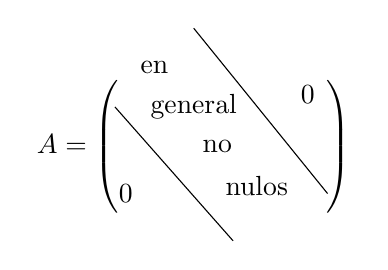
\begin{tikzpicture}
              \node at (0,0) {$A=\begin{pmatrix}
                            & ~~~~ & ~~~~ & 0    \\
                            & ~~~~ & ~~~~ & ~~~~ \\
                            & ~~~~ & ~~~~ & ~~~~ \\
                          0 & ~~~~ & ~~~~ & ~~~~
                      \end{pmatrix}$};
              \node at (-0.5,1) {en};
              \node at (0,0.5) {general};
              \node at (0.3,0) {no};
              \node at (0.8,-0.5) {nulos};
              \draw (0,1.5) -- (1.7,-0.6);
              \draw (-1,0.5) -- (0.5,-1.2);
          \end{tikzpicture}
\end{itemize}

\begin{itemize}[label=\color{red}\textbullet, leftmargin=*]
    \item \color{lightblue} Operaciones con matrices
\end{itemize}
\begin{itemize}[label=$\longrightarrow$]
\item Suma: $A=(a_{\imath\jmath  }), B=(b_{\imath\jmath  })\in M_{m\times
n}(\mathbb{K})$

$A+B=C,~C=(C_{\imath\jmath  })\in M_{m\times
n}(\mathbb{K})\xrightarrow{\hspace{1cm}}C_{\imath\jmath  }=a_{\imath\jmath  }+b_{\imath\jmath  }$

          \underline{Ejemplo:}

          $A=\begin{bmatrix}
                  1 & 2 \\
                  3 & 4
              \end{bmatrix}, B=\begin{bmatrix}
                  5 & 6 \\
                  7 & 8
\end{bmatrix}\xrightarrow{\hspace{2cm}}A+B=\begin{bmatrix}                  6  & 8  \\
                  10 & 12
              \end{bmatrix} $

    \item Producto de un escalar por una matriz.

$\alpha\in\mathbb{K}, A=(a_{\imath\jmath  })\in M_{m\times n}(\mathbb{K})$
          $(\alpha A)=(\alpha a_{\imath\jmath  })$

          $t_j:A=\begin{bmatrix}
                  1 & 2 \\
                  3 & 4
\end{bmatrix}\hspace{0.5cm}\alpha=2\xrightarrow{\hspace{3cm}}(\alpha
A)=\begin{bmatrix}
                  2 & 6 \\
                  6 & 8
              \end{bmatrix}$

\underline{Propiedades de la suma y el producto por escalares}
          \begin{enumerate}
              \item $A+B=B+A$
              \item $(A+B)+C=A+(B+C)$
              \item $(\alpha + \beta)\cdot A=\alpha A+\beta A$
              \item $\alpha(A+B)=\alpha A+\alpha B$
              \item $\alpha(\beta A)=(\alpha\cdot\beta)A$
          \end{enumerate}
    \item Producto de matrices

$A=(a_{\imath\jmath  })\in M_{m\times n}(\mathbb{K}),B=(b_{\imath\jmath  })\in
M_{m\times n}(\mathbb{K})$

          $A\cdot B=(C_{\imath\jmath  })\in M_{m\times k}$

          $C_{\imath\jmath  }=\sum_{k=1}^{n}a_{ik}\cdot b_{kj}$

          \underline{Ejemplo:}

          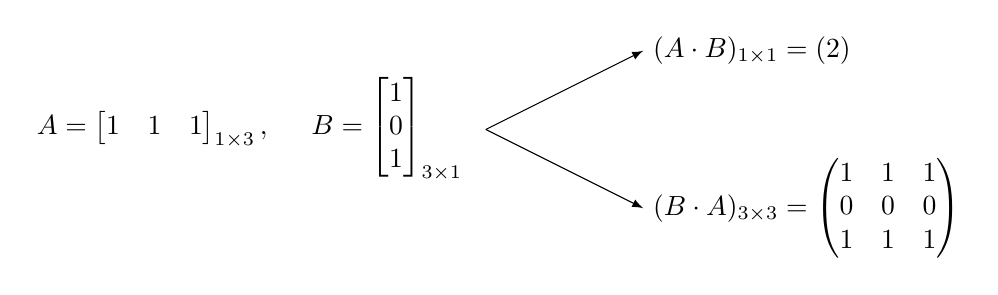
\begin{tikzpicture}
              \node at (0,0) {$A=\begin{bmatrix}
                      1 & 1 & 1
\end{bmatrix}_{1\times 3},\hspace{0.5cm}B=\begin{bmatrix}                      1 \\
                      0 \\
                      1
                  \end{bmatrix}_{3\times 1}$};
\draw[-latex] (3,0) -- (5,1) node[right] {$(A\cdot
B)_{1\times1}=(2)$};
\draw[-latex] (3,0) -- (5,-1) node[right] {$(B\cdot
A)_{3\times3}=
                      \begin{pmatrix}
                          1 & 1 & 1 \\
                          0 & 0 & 0 \\
                          1 & 1 & 1
                      \end{pmatrix}
                  $};
          \end{tikzpicture}
\item[\textbullet] En Python, este producto de matrices se llama
\textbf{dotproduct}.
\item[\textbullet] En Ciencia de Datos también se trabaja con
otros productos diferentes de matrices.

        \underline{Propiedades del producto de matrices}
        \begin{enumerate}
            \item $(A\cdot B)\cdot C=A(B\cdot C)$
            \item $A\cdot 0=0\cdot A=0$
            \item $A(B+C)=A\cdot B+A\cdot C$
            \item $\alpha(A\cdot B)=(\alpha \cdot A)\cdot B$
            \item $A\cdot I=I\cdot A=A$
        \end{enumerate}
\item Como hemos visto antes, el producto de matrices no es
conmutativo, es decir, en general $A\cdot B\neq B\cdot A$.
\end{itemize}
\begin{itemize}[label=\color{red}\textbullet, leftmargin=*]
    \item \color{lightblue} Definición (Traspuesta)
\end{itemize}
Dada $A=(a_{\imath\jmath  })\in M_{m\times n}(\mathbb{K})$, se llama
traspuesta de $A$ a la matriz. \[A^T=(a_{\imath\jmath  })\in M_{n\times
m}(\mathbb{K}),\]es decir, la traspuesta consiste en cambiar
filas por columnas.

Una matriz se dice simétrica si $A=A^T$ y antisimétrica si
$A=-A^T$.

\underline{Ejemplos:}

$A=\begin{bmatrix}
        a & x & y \\
        x & b & z \\
        y & z & c
    \end{bmatrix}~~~~A^T=\begin{bmatrix}
        a & x & y \\
        x & b & z \\
        y & z & c
    \end{bmatrix}$

$A=A^T\xrightarrow{\hspace{1.5cm}}A$ simétrica

$B=\begin{bmatrix}
        0  & \jmath   & -2 \\
        -\jmath  & 0  & 5  \\
        2  & -5 & 0
    \end{bmatrix}~~~~B^T=\begin{bmatrix}
        0  & -\jmath  & 2  \\
        \jmath   & 0  & -5 \\
        -2 & 5  & 0
    \end{bmatrix}$

$B=-B^T\xrightarrow{\hspace{0.5cm}}B$ antisimétrica

\underline{Propiedades de la traspuesta}

\begin{enumerate}
    \item $(A^T)^T=A$
    \item $(A+B)^T=A^T+B^T$
    \item $(\alpha A)^T=\alpha A^T$
    \item $(A\cdot B)^T=B^T\cdot A^T$
\end{enumerate}
\begin{itemize}[label=\color{red}\textbullet, leftmargin=*]
    \item \color{lightblue} Definición (Inversa)
\end{itemize}
Dada $A=(a_{\imath\jmath  })\in M_n(\mathbb{K})$, se dice que $A$ es
invertible si existe una matriz $B\in M_n(\mathbb{K})$ tal que
\[A\cdot B=B\cdot A=I.\]
Dicha matriz $B$, si existe es única y se denota $A^{-1}$.

\underline{Propiedades de la inversa}

Sean $A,B\in M_n(\mathbb{K})$ invertibles. Se tiene:

\begin{enumerate}
\item $A\cdot B$ es invertible y $(A\cdot B)^{-1}=B^{-1}\cdot
A^{-1}$
    \item $A^T$ es invertible y $(A^T)^{-1}=(A^{-1})^T$.
\item Una matriz triangular (superior o inferior) es invertible
si y solo si los elementos de la diagonal son todos no nulos.
\item Sean $u_1,u_2,\hdots,u_m$ vectores de $\mathbb{K}^n$ que
representamos como vectores columna, y sea $A\in
M_n(\mathbb{K})$ invertible. Entonces $u_1,u_2,\hdots,u_m$ son
linealmente independientes si y sólo si $Au_1,Au_2,\hdots,Au_m$
son linealmente independientes.
\end{enumerate}
\underline{Veamos la demostración de 4}
\begin{itemize}[label=$\longrightarrow$]
\item Supongamos que $u_1,u_2,\hdots,u_m$ y veamos que
$Au_1,Au_2,\hdots,Au_m$ son linealmente independientes.
\end{itemize}
Tomamos una combinación lineal nula

\fcolorbox{lightblue}{lightblue!10}{$\lambda_1Au_1,\lambda_2Au_2,\hdots,\lambda_mAu_m=0$}

Por las propiedades del producto de matrices:

\fcolorbox{lightblue}{lightblue!10}{$A(\lambda_1u_1,\hdots,\lambda_mu_m)=0$}

Como $A$ es invertible:

\fcolorbox{lightblue}{lightblue!10}{$A^{-1}A(\lambda_1u_1,\hdots,\lambda_mu_m)=0\xrightarrow{\hspace{0.5cm}}\lambda_1u_1,\hdots,\lambda_mu_m=0$}

Y como $u_1,u_2,\hdots,u_m$ son linealmente independientes.

\fcolorbox{lightblue}{lightblue!10}{$\lambda_1=\lambda_2=\cdots=\lambda_m=0$}

\begin{itemize}[label=\color{red}\textbullet, leftmargin=*]
    \item \color{lightblue} Definición (Matriz ortogonal)
\end{itemize}
Sea $Q\in M_n(\mathbb{R})$. Se dice que $Q$ es ortogonal si es
invertible (o no singular) y si su inversa coincide con su
traspuesta, es decir,
\fcolorbox{lightblue}{lightblue!10}{$Q^T\cdot Q=Q\cdot Q^T=I$}.

Como consecuencia, si $Q$ un ortogonal, entonces las columnas de
$Q$ forman un conjunto ortogonal de vectores.

\underline{Ejemplo}

$Q=\begin{bmatrix}
\textstyle\frac{1}{\sqrt{2}} & \textstyle-\frac{1}{\sqrt{2}} \\\textstyle\frac{1}{\sqrt{2}} & \textstyle\frac{1}{\sqrt{2}}
\end{bmatrix}\hspace{0.5cm}Q^T=\begin{bmatrix}
\textstyle\frac{1}{\sqrt{2}}  & \textstyle\frac{1}{\sqrt{2}} \\\textstyle-\frac{1}{\sqrt{2}} & \textstyle\frac{1}{\sqrt{2}}    \end{bmatrix}$

$Q^T\cdot Q=\begin{bmatrix}
\textstyle\frac{1}{\sqrt{2}}  & \textstyle\frac{1}{\sqrt{2}} \\\textstyle-\frac{1}{\sqrt{2}} & \textstyle\frac{1}{\sqrt{2}}\end{bmatrix}\cdot\begin{bmatrix}
\textstyle\frac{1}{\sqrt{2}} & \textstyle-\frac{1}{\sqrt{2}} \\    \textstyle\frac{1}{\sqrt{2}} & \textstyle\frac{1}{\sqrt{2}}
\end{bmatrix}=\begin{bmatrix}
    1 & 0\\
    0 & 1
\end{bmatrix}\hspace{0.5cm}Q\cdot Q^T=\begin{bmatrix}
\textstyle\frac{1}{\sqrt{2}} & \textstyle-\frac{1}{\sqrt{2}} \\    \textstyle\frac{1}{\sqrt{2}} & \textstyle\frac{1}{\sqrt{2}}
\end{bmatrix}\cdot\begin{bmatrix}
\textstyle\frac{1}{\sqrt{2}}  & \textstyle\frac{1}{\sqrt{2}} \\\textstyle-\frac{1}{\sqrt{2}} & \textstyle\frac{1}{\sqrt{2}}\end{bmatrix}=\begin{bmatrix}
    1 & 0\\
    0 & 1
\end{bmatrix}$

\fcolorbox{lightblue}{lightblue!10}{$u_1=\left(\frac{1}{\sqrt{2}},\frac{1}{\sqrt{2}}\right),
u_2=\left(-\frac{1}{\sqrt{2}},\frac{1}{\sqrt{2}}\right)\longrightarrow\|u_1\|=\|u_2\|=1\longrightarrow
u_1\cdot u_2=0$}
\begin{itemize}[label=\color{red}\textbullet, leftmargin=*]
    \item \color{lightblue} Definición (Traza de una matriz)
\end{itemize}
Dada $A=(a_{\imath\jmath  })\in M_n(\mathbb{K})$, se define la traza de $A$,
denotada $tr(A)=\sum_{i=1}^{n}a_{ii}$, es decir, la traza
escalar que se obtiene sumiendo los elementos de la diagonal.

\underline{Propiedades de la traza}
\begin{enumerate}
    \item $tr(A+B)=tr(A)+tr(B)$
    \item $tr(\alpha A)=\alpha\cdot tr(A)$
    \item $tr(A)=tr(A^T)$
    \item $tr(A\cdot B)=tr(B\cdot A)$
\item $tr(P^{-1}\cdot A\cdot P)=tr(A)$ para cualquier matriz
invertible.
\end{enumerate}
\textcolor{lightblue}{\underline{Matrices por bloques}}

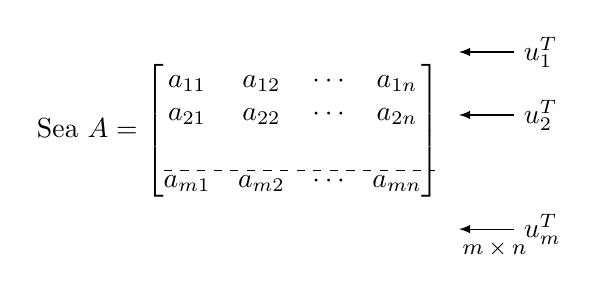
\begin{tikzpicture}
    \node at (0,0) {Sea $A=
    \begin{bmatrix}
        a_{11} & a_{12} & \cdots & a_{1n} \\
        a_{21} & a_{22} & \cdots & a_{2n} \\
         \\
        a_{m1} & a_{m2} & \cdots & a_{mn} \\
    \end{bmatrix}
    $};
    \draw[dashed] (-0.95,-0.5) -- (2.5,-0.5);
    \draw[latex-] (2.8,1) -- (3.5,1) node[right] {$u_1^T$};
    \draw[latex-] (2.8,0.2) -- (3.5,0.2) node[right] {$u_2^T$};
\draw[latex-] (2.8,-1.25) -- (3.5,-1.25) node[right] {$u_m^T$};    \node at (3.25,-1.5) {\footnotesize$m\times n$};
\end{tikzpicture}

En algunas ocasiones conviene escribir $A$ en la forma
$$A=\left[v_1,v_2,\hdots,v_n\right]$$ donde $v_i$ son las
columnas de $A$ o también

$A=\begin{bmatrix}
    u_1^T\\
    \vdots \\
    u_m^T\\
\end{bmatrix}$

Con $u_j^T$ las filas de $A$.

Con esta notación, el producto de una matriz por un vector
columna es:
\begin{center}
    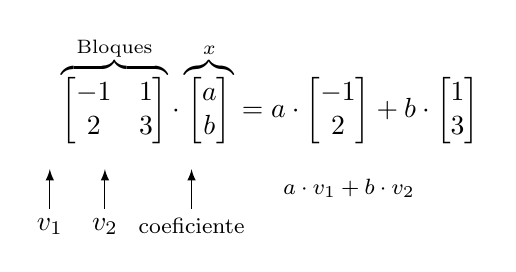
\begin{tikzpicture}
        \node at (0,0) {$\overbrace{
            \begin{bmatrix}
                -1 & 1\\
                2 & 3
            \end{bmatrix}
        }^{\text{Bloques}}\cdot\overbrace{
            \begin{bmatrix}
                a \\
                b
            \end{bmatrix}
        }^{x}=a\cdot\begin{bmatrix}
            -1\\
            2
        \end{bmatrix}+b\cdot\begin{bmatrix}
            1\\
            3
        \end{bmatrix}$};
\draw[latex-] (-2.8,-1) -- (-2.8,-1.5) node[below] {$v_1$};\draw[latex-] (-2.1,-1) -- (-2.1,-1.5) node[below] {$v_2$};\draw[latex-] (-1,-1) -- (-1,-1.5)
node[below] {\footnotesize
coeficiente};
\node[below] at (1,-1) {\footnotesize$a\cdot v_1+b\cdot v_2$};    \end{tikzpicture}
\end{center}
es decir, el producto por la derecha de una matriz $B$ por un
vector columna $x$ es una combinación lineal de las columnas de
$A$ con coeficientes los elementos de $x$.

De manera similar, el producto de un vector fila por una matriz:$$\left[a,b\right]\cdot\begin{bmatrix}
    -1 & 1\\
    2 & 3\\
\end{bmatrix}=a\cdot\left[-1,1\right]+b\cdot\left[2,3\right]$$
es decir, una combinación lineal de las filas de la matriz con
coeficientes los componentes del vector.

Combinando ambas tenemos:
\[\begin{bmatrix}
1 & 4 \\ 
2 & 5 \\ 
3 & 6
\end{bmatrix}\cdot\begin{bmatrix}
7 & 8 & 9 \\ 
10 & 11 & 12
\end{bmatrix}=\begin{bmatrix}
1\\
2\\
3
\end{bmatrix}\cdot\begin{bmatrix}
7 & 8 & 9\\
\end{bmatrix}+\begin{bmatrix}
4 \\ 
5 \\ 
6
\end{bmatrix}\cdot\begin{bmatrix}
10 & 11 & 12
\end{bmatrix}\] que podemos expresar:

$A=\left[v_1,\hdots,v_n\right],~~B=\begin{bmatrix}
u_1^T\\
\vdots\\
u_m^T
\end{bmatrix}~~~~A\cdot B=v_1u_1^T+\cdots+v_nu_m^T$

Es habitual en Machine Learning tener que separar los datos
contenidos en una matriz en varios bloques. Por ejemplo, en
primer lugar los datos de la matriz se dividen en dos bloques:
uno de ellos se utiliza para "entrenar" un modelo de predicción,
y el otro para "testear" cuánto de bueno es dicho modelo. Es lo
que se llama descomponer un \textcolor{lightblue}{dataset} en
\textcolor{lightblue}{data training} y
\textcolor{lightblue}{data test}.

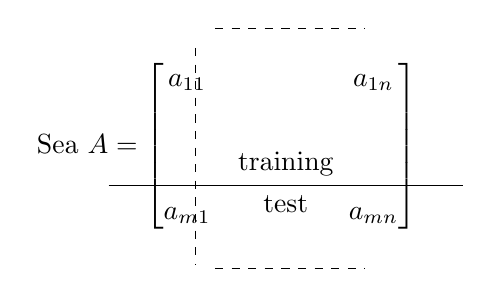
\begin{tikzpicture}
\node at (0,0) {Sea $A=\begin{bmatrix}
a_{11} & ~~ & ~~ & ~~ a_{1n}\\
\\
\\
\\
a_{m1} & ~~ & ~~ & ~~ a_{mn}
\end{bmatrix}$};
\draw[dashed] (-0.15,1.5) -- (1.75,1.5) ;
\draw[dashed] (-0.15,-1.55) -- (1.75,-1.55) ;
\draw[dashed] (-0.4,1.25) -- (-0.4,-1.5) ;
\draw (-1.5, -0.5) -- (3,-0.5) node[midway, above] {training}
node[midway, below] {test};
\end{tikzpicture}

Además en el llamado \textcolor{lightblue}{"supervised
learning"} todas las columnas excepto la última contienen un
tipo de datos llamados \textcolor{lightblue}{"features"} y la
última columna los llamados \textcolor{lightblue}{"labels"}.
Tenemos así:

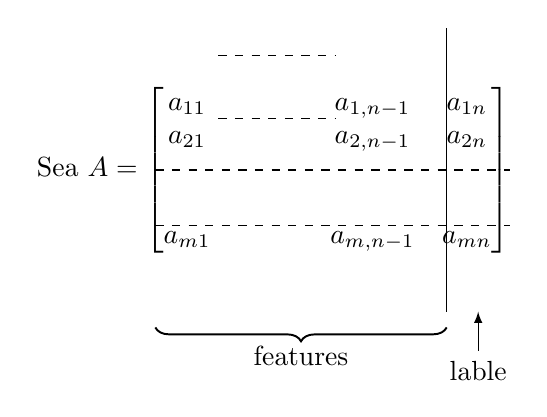
\begin{tikzpicture}
\node at (0,0) {Sea $A=\begin{bmatrix}
a_{11} & ~~ & ~~ & a_{1,n-1} & a_{1n}\\
a_{21} & ~~ & ~~ & a_{2,n-1} & a_{2n}\\
\\
\\

a_{m1} & ~~ & ~~ & a_{m,n-1} & a_{mn}
\end{bmatrix}$};
\draw[dashed] (-0.7,1.45) -- (0.8, 1.45) ;
\draw[dashed] (-0.7,0.65) -- (0.8,0.65) ;
\draw[dashed] (-1.5,0) -- (3,0) ;
\draw[dashed] (-1.5,-0.7) -- (3,-0.7) ;
\draw (2.2,1.8) -- (2.2,-1.8) ;
\draw[decorate,decoration={brace,amplitude=5pt,mirror},line
width=0.7pt]
(-1.5,-2) -- (2.2,-2) node[midway,below=3pt]{features};
\draw[latex-] (2.6,-1.8) -- (2.6,-2.3) node[below] {lable} ;
\end{tikzpicture}


Así, $A$ queda descompuesto en 4 bloques.

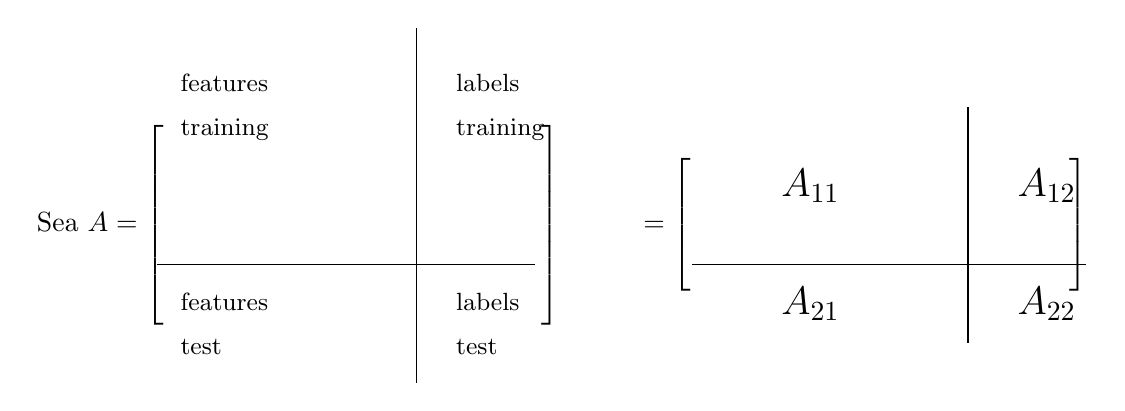
\begin{tikzpicture}
\node at (0,0) {Sea $A=\begin{bmatrix}
~~~~~~~~ & ~~~~~~~~ & ~~~~~~~~ & ~~~~~~~~ \\ 
~~~~~~~~ & ~~~~~~~~ & ~~~~~~~~ & ~~~~~~~~ \\ 
~~~~~~~~ & ~~~~~~~~ & ~~~~~~~~ & ~~~~~~~~ \\ 
~~ & ~~ & ~~ & ~~ \\ 
~~ & ~~ & ~~ & ~~ \\ 
~~ & ~~ & ~~ & ~~
\end{bmatrix}$};
\node at (7.2,0) {$=\begin{bmatrix}
    ~~~~~~~~ & ~~~~~~~~ & ~~~~~~~~ & ~~~~~~~~ \\ 
    ~~~~~~~~ & ~~~~~~~~ & ~~~~~~~~ & ~~~~~~~~ \\ 
    ~~~~~~~~ & ~~~~~~~~ & ~~~~~~~~ & ~~~~~~~~ \\ 
    ~~~~~~~~ & ~~~~~~~~ & ~~~~~~~~ & ~~~~~~~~ \\ 
    \end{bmatrix}$};
\node[text width=4cm] at (0.5,1.5) {\small features\\[4pt]
training};
\node[text width=4cm] at (4,1.5) {\small labels\\[4pt]
training};
\node[text width=4cm] at (0.5,-1.25) {\small features\\[4pt]
test};
\node[text width=4cm] at (4,-1.25) {\small labels\\[4pt] test};
\draw (1.5,2.5) -- (1.5,-2);
\draw (-1.8,-0.5) -- (3,-0.5);
\draw (8.5,1.5) -- (8.5,-1.5);
\draw (5,-0.5) -- (10,-0.5);
\node at (6.5,0.5) {\Large $A_{11}$};
\node at (6.5,-1) {\Large $A_{21}$};
\node at (9.5,0.5) {\Large $A_{12}$};
\node at (9.5,-1) {\Large $A_{22}$};
\end{tikzpicture}

El producto de matrices opera por bloques de igual manera a como
se hace por entradas.

\textcolor{lightblue}{\underline{Operaciones y matrices
elementales}}

Muchos de los cálculos habituales del Álgebra Lineal requieren
realizar las siguientes \textcolor{lightblue}{"operaciones
elementales"} sobre las filas y/o columnas de una matriz:

\begin{enumerate}
    \item Intercambiar dos filas (columnas)
    \item Multiplicar una fila (columna) por un escalar.
\item Añadir a cada fila (columna) otra fila (columna)
multiplicada por un escalar.
\end{enumerate}

Estas operaciones se pueden realizar de manera sistemática
multiplicando la matriz en cuestión por una determinada matriz,
que llamaremos \textcolor{lightblue}{matriz elemental}.

Hay tres tipos de matrices elementales:

\begin{enumerate}
\item Matriz de \textcolor{lightblue}{permutación simple} (Pst)
obtenida al intercambiar las filas (o columnas) \emph{st}.
    
    \underline{Ejemplo:}

    $A=\begin{bmatrix}
        a_{11} & a_{12}\\
        a_{21} & a_{22}\\
    \end{bmatrix}; P_{12}=\begin{bmatrix}
        0 & 1\\ 
        1 & 0
    \end{bmatrix}\begin{array}{l}
        \longleftarrow 1,~~1\longrightarrow 2\\
        \longleftarrow 1,~~2\longrightarrow 1\\
    \end{array}$

    $P_{12}\cdot A=\begin{bmatrix}
        0 & 1\\
        1 & 0
    \end{bmatrix}\cdot    \begin{bmatrix}
        a_{11} & a_{12}\\
        a_{21} & a_{22}\\
    \end{bmatrix}=    \begin{bmatrix}
        a_{21} & a_{22}\\
        a_{11} & a_{12}\\
    \end{bmatrix}$

    $    \begin{bmatrix}
        a_{11} & a_{12}\\
        a_{21} & a_{22}\\
\end{bmatrix}\overset{F_1\longleftrightarrow
F_2}{\xrightarrow{\hspace*{2cm}}} \begin{bmatrix}
        a_{21} & a_{22}\\
        a_{11} & a_{12}\\
    \end{bmatrix};$
    \item Matriz de \textcolor{lightblue}{dilatación} $D_s(r)$
    
    $D_2(5)=\begin{bmatrix}
        1 & 0 \\
        0 & 1
    \end{bmatrix}; ~~D_2(5)\cdot A=\begin{bmatrix}
        1 & 0\\
        0 & 1\\
    \end{bmatrix}\cdot    \begin{bmatrix}
        a_{11} & a_{12}\\
        a_{21} & a_{22}\\
    \end{bmatrix}
    =    \begin{bmatrix}
        a_{11} & a_{12}\\
        5a_{21} & 5a_{22}\\
    \end{bmatrix}$

    \item Matriz de \textcolor{lightblue}{adición}:
    
$S_{st}(r)=$ a la fila $s$ se le suma la fila $t$ multiplicada
por $r$.

    $S_{12}(2)=\begin{bmatrix}
        1 & 2\\
        0 & 1 
    \end{bmatrix}; S_{12}(2)\cdot A=\begin{bmatrix}
        1 & 2\\
        0 & 1
    \end{bmatrix}\cdot    \begin{bmatrix}
        a_{11} & a_{12}\\
        a_{21} & a_{22}\\
    \end{bmatrix}=    \begin{bmatrix}
        a_{11}+2a_{21} & a_{12}+2a_{22}\\
        a_{21} & a_{22}\\
    \end{bmatrix};$
\end{enumerate}
\begin{itemize}[label=\color{red}\textbullet, leftmargin=*]
    \item \color{lightblue} Propiedades:
\end{itemize}
Las matrices elementales son invertibles. Además:
\begin{enumerate}[label=\arabic*)]
    \item $P_{st}^{-1}=Pst$
    \item $Ds(r)^{-1}=Ds\frac{1}{r}$
    \item $S_{st}(r)^{-1}=S_{st}(-r)$
\end{enumerate}
En algunas ocasiones es necesario combinar operaciones
elementales fila y también columna sobre una misma matriz $A$.
De esta forma obtenemos una nueva matriz $B$, equivalente a $A$,
y que se expresan en la forma.

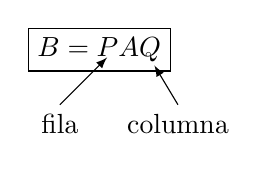
\begin{tikzpicture}
\node[draw=black, rectangle] {$B=PAQ$};
\draw[latex-] (0.1,-0.1) -- (-0.5,-0.7) node[below] {fila};
\draw[latex-] (0.7,-0.2) -- (1,-0.7) node[below] {columna};
\end{tikzpicture}
\begin{itemize}[label=\color{red}\textbullet, leftmargin=*]
    \item \color{lightblue} Definición (Matriz de permutación)
\end{itemize}
Llamaremos matriz de permutación $P$ a aquella que se expresa
como producto de matrices de permutación elementales.

\textcolor{lightblue}{\underline{Matrices escalonadas. Rango}}
\begin{itemize}[label=\color{red}\textbullet, leftmargin=*]
    \item \color{lightblue} Definición
\end{itemize}
Dada una matriz se llama \textcolor{lightblue}{pivote} de una
fila no nula a la primera entrada (contando izquierda a derecha)
no nula a esa fila. Se dice que la \textcolor{lightblue}{matriz}
es \textcolor{lightblue}{escalonada} por filas si:
\begin{enumerate}[label=\arabic*)]
\item El pivote de cada fila no nula está estrictamente a la
derecha del pivote de la fila anterior.
    \item Las filas nulas, si las hay, son las últimas.
\end{enumerate}
Se dice que la matriz es \textcolor{lightblue}{escalonada
reducida} por filas si además:
\begin{enumerate}
\item[1º)] El pivote de cada fila no nula vale 1.
\item[2º)] Cada pivote es el único no nulo de su columna.
\end{enumerate}
De manera análoga se puede definir el concepto de matriz
escalonada (reducida) por columnas.

\underline{Ejemplo}

$A=\underbrace{\begin{bmatrix}
2 & 0 & 0 & 5 \\ 
0 & 1 & 0 & 2 \\ 
0 & 3 & 1 & 4
\end{bmatrix} }_{\text{No escalonada}}$\hspace{0.5cm}
$B=\underbrace{\begin{bmatrix}
1 & 2 & 0 & 4 & 5 \\ 
0 & 0 & -1 & 1 & 5 \\ 
0 & 0 & 0 & 2 & 2
\end{bmatrix} }_{\text{Escalonada pero no
reducida}}$\hspace{0.5cm} $C=\underbrace{\begin{bmatrix}
1 & 0 & 2 & 0 & 5 \\ 
0 & 1 & 6 & 0 & 2 \\ 
0 & 0 & 0 & 1 & 4
\end{bmatrix}}_{\text{Escalonada reducida}}$
\begin{itemize}[label=\color{red}\textbullet, leftmargin=*]
    \item \color{lightblue} Teorema (Factorización $PAQ$)
\end{itemize}
Toda matriz $A$ es equivalente a una matriz de la forma 
\begin{center}
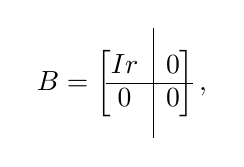
\begin{tikzpicture}
\node at (0,0) {$B=\begin{bmatrix}
Ir &  0 \\ 
0 & 0
\end{bmatrix},$};
\draw (0.4,0.7) -- (0.4,-0.7);
\draw (-0.2,0) -- (0.9,0);
\end{tikzpicture}
\end{center}
es decir, existen matrices invertibles $P$ y $Q$ tales que 

\fcolorbox{lightblue}{lightblue!10}{$B=PAQ$}

\begin{itemize}[label=$\longrightarrow$]
\item La forma de llegar de $A$ a $B$ es realizando operaciones
elementales. Este proceso se llama
\textcolor{lightblue}{eliminación gaussiana}
\end{itemize}

Al número $r$, es decir, al número de filas no nulas que
resultan después de escalonar una matriz se le llama
\textcolor{lightblue}{rango} de la matriz y se denota por
$r=\rg(A)$

\underline{Ejemplo}

$A=\begin{bmatrix}
1 & 2 & -1 & 2 \\ 
2 & 4 & 1 & 1 \\ 
3 & 6 & 0 & 3
\end{bmatrix} $

Hacemos operaciones elementales fila con la matriz.

$(A|I_3)=\left[\begin{array}{cccc:ccc}
1 & 2 & -1 & 2 & 1 & 0 & 0 \\ 
2 & 4 & 1 & 1 & 0 & 1 & 0 \\ 
3 & 6 & 0 & 3 & 0 & 0 & 1
\end{array} \right]\overset{F_2\rightarrow
F_2-2F_1}{\underset{F_3\rightarrow
F_3-3F_1}{\xrightarrow{\hspace{1.5cm}}}}\left[\begin{array}{cccc:ccc}
1 & 2 & -1 & 2 & 1 & 0 & 0 \\ 
0 & 0 & 3 & -3 & -2 & 1 & 0 \\ 
0 & 0 & 3 & -3 & -3 & 0 & 1
\end{array} \right]\overset{F_3\rightarrow
F_3-F_2}{\xrightarrow{\hspace{1.5cm}}}$

$\left[\begin{array}{cccc:ccc}
1 & 2 & -1 & 2 & 1 & 0 & 0 \\ 
0 & 0 & 3 & -3 & -2 & 1 & 0 \\ 
0 & 0 & 0 & 0 & -1 & -1 & 1
\end{array} \right]$

El rango de $A$ es $r=\rg(A)=2$

Seguimos haciendo operaciones fila para conseguir la forma
reducida, donde los pivotes son 1s y cada pivote es el único
elemento no nulo de su columna.

$\overset{F_2\rightarrow
\frac{1}{3}F_2}{\xrightarrow{\hspace{1.5cm}}}\left[\begin{array}{cccc:ccc}
1 & 2 & -1 & 2 & 1 & 0 & 0 \\ 
0 & 0 & 1 & -1 & -\textstyle\frac{2}{3} & \textstyle\frac{1}{3}
& 0 \\
0 & 0 & 0 & 0 & -1 & -1 & 1
\end{array} \right]\overset{F_1\rightarrow
F_1+F_2}{\xrightarrow{\hspace{1.5cm}}}\left[\begin{array}{cccc:ccc}
1 & 2 & 0 & 1 & \textstyle\frac{1}{3} & \textstyle\frac{1}{3} &
0 \\
0 & 0 & 1 & -1 & \textstyle-\frac{2}{3} & \textstyle\frac{1}{3}
& 0 \\
0 & 0 & 0 & 0 & -1 & -1 & 1
\end{array} \right]$

Se tiene que 

$\begin{bmatrix}
1 & 2 & 0 & 1 \\ 
0 & 0 & 1 & -1 \\ 
0 & 0 & 0 & 0
\end{bmatrix}=PA$, con $\begin{bmatrix}
\textstyle\frac{1}{3} & \textstyle\frac{1}{3} & 0 \\ 
-\textstyle\frac{2}{3} & \textstyle\frac{1}{3} & 0 \\ 
-1 & -1 & 1	
\end{bmatrix} $

Ahora realizamos operaciones columna para obtener la forma
$\left[\begin{array}{c|c}
Ir & 0 \\ 
\hline
0 & 0
\end{array} \right]$

$\begin{bmatrix}
1 & 2 & 0 & 1 \\ 
0 & 0 & 1 & -1 \\ 
0 & 0 & 0 & 0 \\ \hdashline
1 & 0 & 0 & 0 \\ 
0 & 1 & 0 & 0 \\ 
0 & 0 & 1 & 0 \\ 
0 & 0 & 0 & 1
\end{bmatrix}\overset{C_2\longleftrightarrow
C_3}{\xrightarrow{\hspace{1.5cm}}}\begin{bmatrix}
1 & 0 & 2 & 1 \\ 
0 & 1 & 0 & -1 \\ 
0 & 0 & 0 & 0 \\ \hdashline
1 & 0 & 0 & 0 \\ 
0 & 1 & 0 & 0 \\ 
0 & 0 & 1 & 0 \\ 
0 & 0 & 0 & 1
\end{bmatrix}\overset{C_3\rightarrow
C_3-2C_1}{\underset{C_4\rightarrow
C_4-C_1}{\xrightarrow{\hspace{1.5cm}}}}\begin{bmatrix}
1 & 0 & 0 & 0 \\ 
0 & 1 & 0 & 0 \\ 
0 & 0 & 0 & 1 \\ 
\hdashline
1 & 0 & -2 & -1 \\ 
0 & 1 & 0 & 0 \\ 
0 & 0 & 1 & 0 \\ 
0 & 0 & 0 & 1
\end{bmatrix} $

$Q=\begin{bmatrix}
1 & 0 & -2 & -1 \\ 
0 & 0 & 1 & 0 \\ 
0 & 1 & 0 & 1 \\ 
0 & 0 & 0 & 1
\end{bmatrix} $\hspace{2cm} $\left[\begin{array}{c|c}
Ir_2 & 0 \\ \hline
0 & 0
\end{array} \right]=PAQ$

\textcolor{lightblue}{\underline{Sistemas de ecuaciones}}
\begin{itemize}[label=\color{red}\textbullet, leftmargin=*]
    \item \color{lightblue} Definición
\end{itemize}
Un sistema lineal de $m$-ecuaciones con $n$-incógnitas es un
sistema del tipo

$(*)\left\lbrace
\begin{array}{l}
a_{11}x_1+a_{12}x_2+\cdots+a_{1n}x_n=b_1\\
a_{21}x_1+a_{22}x_2+\cdots+a_{2n}x_n=b_2\\
\hdashline
a_{m1}x_1+a_{m2}x_2+\cdots+a_{mn}x_n=b_m\\
\end{array}
\right.$

que en forma matricial escribimos como 

$(*)$\hspace{1cm}$Ax=b$

donde 
\begin{itemize}
\item $A=(a_{\imath\jmath  })$ es la matriz del sistema
\item $b=(b_{\imath\jmath  })$ es el término independiente
\item $x=(x_{\imath\jmath  })$ es el vector incógnita
\end{itemize}
El sistema $(*)$ se dice:
\begin{itemize}
\item Homogéneo: si $b=0$
\item Incompatible: si no tiene solución
\item Compatible determinado: si tiene una única solución.
\item Compatible indeterminado: infinitas soluciones.
\end{itemize}
\begin{itemize}[label=\color{red}\textbullet, leftmargin=*]
    \item \color{lightblue}Teorema (Rouché-Frobenius)
\end{itemize}

Consideremos el sistema $(*)$ y sea $(A|b)$ la llamada matriz
ampliada. Entonces:
\begin{enumerate}[label=\arabic*)]
\item Si $r(A)=r(A|b)=$ número de incógnitas, entonces el
sistema $(*)$ es compatible determinado (CD).
\item Si $r(A)=r(A|b)<$ número de incógnitas, entonces el
sistema $(*)$ es compatible indeterminado (CI) y la solución
depende del número de incógnitas $-$ $r(A)$ parámetros.
\item Si $r(A)\neq r(A|b)$, el sistema $(*)$ es incompatible.\end{enumerate}
\begin{itemize}[label=\color{red}\textbullet, leftmargin=*]
\item \color{lightblue} Resolución de sistemas lineales mediante
el método de Gauss
\end{itemize}
Consiste en realizar operaciones elementales fila sobre la
matriz ampliada $(A|b)$ hasta conseguir una matriz escalonada,
cuyo sistema asociado tiene la misma solución que el sistema
original, pero que se resuelve muy fácilmente.

\underline{Ejemplo}

$\left.\begin{array}{l}
2x+y+2z+3t=6\\
x+2y-2z-t=3\\
4x+5y-2z+t=12
\end{array}\right\rbrace(A|b)=\left[\begin{array}{cccc:c}
2 & 1 & 2 & 3 & 6 \\ 
1 & 2 & 2 & -1 & 3 \\ 
4 & 5 & -2 & 1 & 12
\end{array} \right]\overset{F_1\longleftrightarrow
F_2}{\xrightarrow{\hspace{1.5cm}}}\left[\begin{array}{cccc:c}
1 & 2 & 2 & -1 & 3 \\ 
2 & 1 & 2 & 3 & 6 \\ 
4 & 5 & -2 & 1 & 12
\end{array} \right]\overset{F_2\rightarrow
F_2-2F_1}{\underset{F_3\rightarrow
F_3-4F_1}{\xrightarrow{\hspace{2cm}}}}$

$\left[\begin{array}{cccc:c}
1 & 2 & 2 & -1 & 3 \\ 
0 & -3 & 6 & 5 & 0 \\ 
0 & -3 & 6 & 5 & 0
\end{array} \right]\overset{F_3\rightarrow
F_3-F_3}{\xrightarrow{\hspace{1.5cm}}}\left[\begin{array}{cccc:c}
1 & 2 & 2 & -1 & 3 \\ 
0 & -3 & 6 & 5 & 0 \\ 
0 & 0 & 0 & 0 & 0
\end{array} \right]$

\begin{wrapfigure}{r}{0.3\textwidth}
	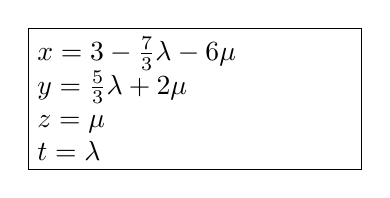
\begin{tikzpicture}
\node[draw=black, rectangle, text width=4cm]
{$x=3-\frac{7}{3}\lambda-6\mu$\\
	$y=\frac{5}{3}\lambda+2\mu$\\
	$z=\mu$\\
	$t=\lambda$};
	\end{tikzpicture}
\end{wrapfigure}

$\rg(A)=2=\rg(A|b)<4=$ nº de incógnitas $\longrightarrow$ S.C.I
tomamos 4-2 parámetros $t=\lambda,~z=\mu$

$\left.\begin{array}{r}
x+2y-2\mu-\lambda=3\\
-3y+6\mu+5\lambda=0
\end{array}\right\rbrace$

$y=2\mu+\frac{5}{3}\lambda$

$x=3-2\left(2\mu+\frac{5}{3}\lambda\right)+2\mu+\lambda=3-4\mu-\frac{10}{3}\lambda+2\mu+\lambda=3-6\mu-\frac{7}{3}\lambda$

\begin{itemize}[label=\color{red}\textbullet, leftmargin=*]
\item \color{lightblue} Cálculo de la inversa de una matriz
mediante eliminación gaussiana
\end{itemize}

\begin{itemize}
\item[$\longrightarrow$] Método: realizar operaciones
elementales fila sobre la matriz $(A|I)$ hasta conseguir que a
la izquierda aparezca la identidad. La matriz que resulta a la
derecha es $A^{-1}$
\end{itemize}

\underline{Ejemplo}

$A=\begin{bmatrix}
1 & 2 & -1 \\ 
2 & 4 & 1 \\ 
3 & 7 & 0
\end{bmatrix} $

$\left[\begin{array}{ccc:ccc}
1 & 2 & -1 & 1 & 0 & 0 \\ 
2 & 4 & 1 & 0 & 1 & 0 \\ 
3 & 7 & 0 & 0 & 0 & 1
\end{array} \right]\overset{F_2\rightarrow
F_2-2F_1}{\underset{F_3\rightarrow
F_3-3F_1}{\xrightarrow{\hspace{1.5cm}}}}\left[\begin{array}{ccc:ccc}
1 & 2 & -1 & 1 & 0 & 0 \\ 
0 & 0 & 3 & -2 & 1 & 0 \\ 
0 & 1 & 3 & -3 & 0 & 1
\end{array} \right]\overset{F_2\longleftrightarrow
F_3}{\xrightarrow{\hspace{1.5cm}}}\left[\begin{array}{ccc:ccc}
1 & 2 & -1 & 1 & 0 & 0 \\ 
0 & 1 & 3 & -3 & 0 & 1 \\ 
0 & 0 & 3 & -2 & 1 & 0
\end{array} \right]$

$\overset{F_2\rightarrow F_2-F_3}{\underset{F_3\rightarrow
\frac{1}{3}F_3}{\xrightarrow{\hspace{1.5cm}}}}\left[\begin{array}{ccc:ccc}
1 & 2 & -1 & 1 & 0 & 0 \\ 
0 & 1 & 0 & -1 & -1 & 1 \\ 
0 & 0 & 1 & -\textstyle\frac{2}{3} & \textstyle\frac{1}{3} & 0
\end{array} \right]\overset{F_1\rightarrow
F_1+F_3}{\xrightarrow{\hspace{1.5cm}}}\left[\begin{array}{ccc:ccc}
1 & 2 & 0 & \textstyle\frac{1}{3} & \textstyle\frac{1}{3} & 0 \\0 & 1 & 0 & -1 & -1 & 1 \\ 
0 & 0 & 1 & -\textstyle\frac{2}{3} & \textstyle\frac{1}{3} & 0
\end{array} \right]\overset{F_1\rightarrow
F_1-2F_2}{\xrightarrow{\hspace{1.5cm}}}$

$\left[\begin{array}{ccc:ccc}
1 & 0 & 0 & \textstyle\frac{7}{3} & \textstyle\frac{7}{3} & -2
\\
0 & 1 & 0 & -1 & -1 & 1 \\ 
0 & 0 & 1 & -\textstyle\frac{2}{3} & \textstyle\frac{1}{3} & 0
\end{array} \right]\hspace{2cm}A^{-1}=\begin{bmatrix}
\textstyle\frac{7}{3} & \textstyle\frac{7}{3} & -2 \\ 
-1 & -1 & 1 \\ 
-\textstyle\frac{2}{3} & \textstyle\frac{1}{3} & 0
\end{bmatrix} $

\textcolor{lightblue}{\underline{Determinantes}}

Sea $A\in M_2(\mathbb{K})$. Se define el determinante de $A$,
denotado $|A|$ o $\dt(A)$, como

$\begin{vmatrix}
a_{11} & a_{12} \\ 
a_{21} & a_{22}
\end{vmatrix}=a_{11}a_{22}-a_{12}a_{21}$

Sea $A\in M_3(\mathbb{K})$. Se define el determinante de $A$
mediante la llamada regla de Sarrus como

$\begin{vmatrix}
a_{11} & a_{12} & a_{13} \\ 
a_{21} & a_{22} & a_{23} \\ 
a_{31} & a_{32} & a_{33}
\end{vmatrix}=a_{11}a_{22}a_{33}+a_{12}a_{23}a_{31}+a_{13}a_{21}a_{32}-\left(a_{13}a_{22}a_{31}+a_{12}a_{21}a_{33}+a_{11}a_{23}a_{32}\right)$

Para matrices de orden superior, el determinante se define de
manera recurrente.

\begin{itemize}[label=\color{red}\textbullet, leftmargin=*]
    \item \color{lightblue} Definición
\end{itemize}

Sea $A=\left(a_{\imath\jmath  }\right)\in M_n(\mathbb{K})$.

Se llama \textcolor{lightblue}{menor complementario} el elemento
$a_{\imath\jmath  }$ al determinante $\left(\left|A_{\imath\jmath  }\right|\right)$ de
la submatriz $A_{\imath\jmath  }$ que se obtiene la fila $i$ y la columna
$j$ de la matriz original $A$.

Se llama \textcolor{lightblue}{adjunto} de $a_{\imath\jmath  }$, denotado
$\triangle_{\imath\jmath  }$, al escalar
$\Delta_{\imath\jmath  }=(-1)^{i+\jmath }\cdot|A_{\imath\jmath  }|$.

\underline{Ejemplo}

\renewcommand{\arraystretch}{1}
\setlength{\arraycolsep}{10pt}

$A=\begin{bmatrix}
1 & 2 & 3 & 4 \\ 
2 & 3 & 4 & 5 \\ 
2 & 0 & 1 & 1 \\ 
4 & 3 & 1 & 2
\end{bmatrix}\hspace{2cm}A_{23}=\begin{vmatrix}
1 & 2 & 4 \\ 
2 & 0 & 1 \\ 
4 & 3 & 2
\end{vmatrix}=21\longrightarrow\Delta_{23}=(-1)^{2+3}\cdot
A_{23}=-21$

\begin{itemize}[label=\color{red}\textbullet, leftmargin=*]
    \item \color{lightblue}Definición
\end{itemize}
Sea $A\in M_n(\mathbb{K})$. El determinante de $A$ se aplica de
forma recurrente como
\begin{itemize}
\item Si $n=1,~|(a)|=a$
\item Si
$n>1,|A|=a_{\imath\jmath  }\Delta_{\imath\jmath  }+a_{i2}\Delta_{i2}+\cdots+a_{in}\Delta_{in}$
\end{itemize}

\underline{Ejemplo}

$A=\begin{bmatrix}
1 & 2 & 4 \\ 
2 & 0 & 1 \\ 
4 & 3 & 2
\end{bmatrix} $

Desarrollado por la primera fila:

$|A|=1\cdot\begin{vmatrix}
0 & 1 \\ 
3 & 2
\end{vmatrix}-2\cdot\begin{vmatrix}
2 & 1 \\ 
4 & 2
\end{vmatrix} +4\cdot\begin{vmatrix}
2 & 0 \\ 
4 & 3
\end{vmatrix}=-3-2(4-4)+4\cdot6=21$

Y si desarrollamos por la segunda columna:

$|A|=-2\cdot\begin{vmatrix}
2 & 1 \\ 
4 & 2
\end{vmatrix}+0\cdot\begin{vmatrix}
~~ & ~~ \\ 
~ & ~
\end{vmatrix}-3\cdot\begin{vmatrix}
1 & 4 \\ 
2 & 1
\end{vmatrix}=-3\cdot(-7)=21$

\hspace{0.5cm}\underline{Propiedades básicas}
\begin{enumerate}[label=\arabic*), leftmargin=*]
    \item $|A|=|A^T|$
    \item $|A\cdot B|=|A|\cdot|B|$
\item $A$ no es singular si y sólo si $|A|\neq0$. En este caso
$|A^{-1}|=\frac{1}{|A|}$
    \item Si $Q$ es ortogonal, entonces $|Q|=I\cdot 1$.
\end{enumerate}

\begin{itemize}[label=$\longrightarrow$]
\item Veamos 4)
\end{itemize}
Si $Q$ es ortogonal, entonces $Q^{-1}=Q^T$.

$I=Q\cdot Q^{-1}\longrightarrow 1=|I|=|Q\cdot
Q^{-1}|=|Q|\cdot|Q^{-1}|=|Q|\cdot|Q^{T}|=|Q|\cdot|Q|=|Q|^2$

Por tanto $Q=\pm1$

\hspace{1cm}\underline{Propiedades de los determinantes y las
operaciones elementales}

\begin{enumerate}[label=\arabic*), leftmargin=*]
\item
$\left|\left[u_1,u_2,\hdots,u_j+u_j',\hdots,u_n\right]\right|=\left|\left[u_1,\hdots,u_j,\hdots,u_n\right]\right|+\left|\left[u_1,\hdots,u_j',\hdots,u_n\right]\right|$
\item $\left|\left[u_1,u_2,\hdots,\alpha
u_j,\hdots,u_n\right]\right|=\alpha\left|\left[u_1,u_2,\hdots,u_n\right]\right|$
\item $\left|\left[u_1,\hdots,u_i,\hdots,u_j,\hdots,
u_n\right]\right|=-\left|\left[u_1,\hdots,u_j,\hdots,u_i,\hdots,
u_n\right]\right|$
\item Si a una columna (o fila) se le suma otra columna (o fila)
multiplicada por un escalar, entonces el determinante no cambia.
\end{enumerate}

\underline{Ejemplo}

$\begin{vmatrix}
a & a+1 & a+2 \\ 
a+3 & a+4 & a+5 \\ 
a+6 & a+7 & a+8
\end{vmatrix} \overset{F_2\rightarrow
F-2-F_1}{\underset{F_3\rightarrow
F_3-F_1}{\xrightarrow{\hspace{1.5cm}}}}\begin{vmatrix}
a & a+1 & a+2 \\ 
3 & 3 & 3 \\ 
6 & 6 & 6
\end{vmatrix}\xrightarrow{\hspace{1.5cm}}2\cdot\begin{vmatrix}
a & a+1 & a+2 \\ 
3 & 3 & 3 \\ 
3 & 3 & 3
\end{vmatrix}\overset{F_3\rightarrow
F-2-F_2}{\xrightarrow{\hspace{1.5cm}}}$

$2\cdot\begin{vmatrix}
a & a+1 & a+2 \\ 
3 & 3 & 3 \\ 
0 & 0 & 0
\end{vmatrix}=0$

\hspace{1cm}\underline{Resolución de sistemas lineales usando
determinantes}

Consideramos el sistema $Ax=b$ y denotamos por $\Delta_i$ el
determinante de la matriz $A$ donde se ha sustituido la columna
$\imath$-ésima por $b$, es decir,

\begin{center}
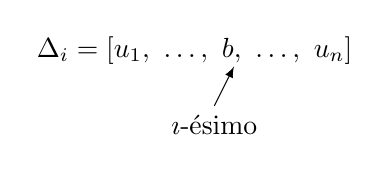
\begin{tikzpicture}
\node {$\Delta_i=\left[u_1,~\hdots,~b,~\hdots,~u_n\right]$};
\draw[latex-] (0.5,-0.2) -- (0.25,-0.7) node[below] {$\imath$-ésimo};\end{tikzpicture}
\end{center}
Entonces, si $|A|\neq0$ se cumple $x_i=\frac{a_i}{|A|}$ (regla
de Cramer)

\underline{Ejemplo}

$\left.\begin{array}{r}
x+y+z=1\\
-x\quad+z=1\\
x+y-z=1
\end{array}\right\rbrace\xrightarrow{\hspace{1.5cm}}|A|=\begin{vmatrix}
1 & 1 & 1 \\ 
-1 & 0 & 1 \\ 
1 & 1 & -1
\end{vmatrix}=1-1-(1+1)=-2$

$\Delta_1=\begin{vmatrix}
1 & 1 & 1 \\ 
1 & 0 & 1 \\ 
1 & 1 & -1
\end{vmatrix}=1+1-(1-1)=2$

$\Delta_2=\begin{vmatrix}
1 & 1 & 1 \\ 
-1 & 1 & 1 \\ 
1 & 1 & -1
\end{vmatrix}=-1+1-1-(1+1+1)=-4$

$\Delta_3=\begin{vmatrix}
1 & 1 & 1 \\ 
-1 & 0 & 1 \\ 
1 & 1 & 1
\end{vmatrix}=0$

$x_1=\frac{\Delta_1}{|A|}=\frac{2}{-2}=-1,~x_2=\frac{\Delta_2}{|A|}=\frac{-4}{-2}=2,~x_3=\frac{\Delta_3}{|A|}=0$.

\textcolor{lightblue}{\underline{Cálculo de la inversa mediante
determinantes}}
\begin{itemize}[label=\color{red}\textbullet, leftmargin=*]
    \item \color{lightblue} Definición (Matriz adjunta)
\end{itemize}
Sea $A\in M_n(\mathbb{K})$. Se llama matriz adjunta de $A$,
denotada $\tilde{A}$, a la matriz cuyas entradas son los adjuntos
de las entradas de $A$, es decir, si $A=(a_{\imath\jmath  })$, entonces
$\tilde{A}=(\Delta_{\imath\jmath  })$.
\begin{itemize}[label=\color{red}\textbullet, leftmargin=*]
    \item \color{lightblue} Proposición
\end{itemize}
Si $A\in M_n(\mathbb{K})$ es invertible, entonces
$A^{-1}=\frac{1}{|A|}\cdot\tilde{A}^T$

\underline{Ejemplo}

Sea $Q=\begin{bmatrix}
a & c \\ 
b & d
\end{bmatrix} $ una matriz ortogonal con determinante $|Q|=+1$

Vamos a calcular su inversa:

$\begin{array}{ll}
\Delta_{11}=|d|=d, & \Delta_{12}=-b\\
\Delta_{21}=-c & \Delta_{22}=a
\end{array}$

Por tanto,

$Q^{-1}=\frac{1}{\underbrace{|Q|}_{1}} \cdot\begin{bmatrix}
d & -c \\ 
-b & a
\end{bmatrix}=\begin{bmatrix}
d & -c \\ 
-b & a
\end{bmatrix}$

y como $Q^T=Q^{-1}$, al set $Q$ ortogonal, $d=a,~-c=b$.

En resumen, 

$Q^{-1}=\begin{bmatrix}
a & b \\ 
-b & a
\end{bmatrix}$ con $a^2+b^2=1$

\newpage

\section{Factorizaciones LU y Cholesky}

\textcolor{lightblue}{\underline{Álgebra lineal computacional}}

Problemas básicos:

\begin{itemize}
\item Resolución de sistemas lineales
\item Cálculo de la inversa
\item Cálculo de determinantes
\item Cálculo de vectores propios
\end{itemize}
Todo ello para \textcolor{lightblue}{matrices de gran tamaño}.

\textcolor{lightblue}{\underline{Ejemplo:}} Cálculo del
determinante de una matriz cuadrada de tamaño $n=100$.

Usando el método estudiado hasta ahora, el número de operaciones
necesarias es aproximadamente.
\begin{center}
\fcolorbox{lightblue}{lightblue!10}{$100!\approx9.3\times10^{157}$}
\end{center}
El Marenostrum 4 de Barcelona Supercomputing Center (uno de los
más potentes a nivel mundial) tiene una capacidad de cálculo de
\begin{center}
\fcolorbox{lightblue}{lightblue!10}{11.15 Petaflops (11,500
billones de operaciones por segundo).}
\end{center}
Por tanto, para calcular el determinante anterior tardaría
$\dfrac{9.3\cdot10^{157}}{1.115\cdot10^{16}}$ segundos que son
$2.6\cdot10^{134}$ años.

En cambio, usando la factorización $LU$ que veremos a
continuación, este cálculo es casi instantáneo.

\textcolor{lightblue}{\underline{Factorización $LU$}}

Dada una matriz $A\in M_{n\times m}(\mathbb{K})$, se llama
factorización $LU$ a una factorización de la forma
\begin{center}
\fcolorbox{lightblue}{lightblue!10}{$A=LU$}
\end{center}
donde $L$ es una matriz triangular inferior con $1s$ en la
diagonal principal, y $U$ es una matriz triangular superior.
$(L\equiv\text{Lower},~U\equiv\text{Upper})$. Si $A$ es
cuadrada:

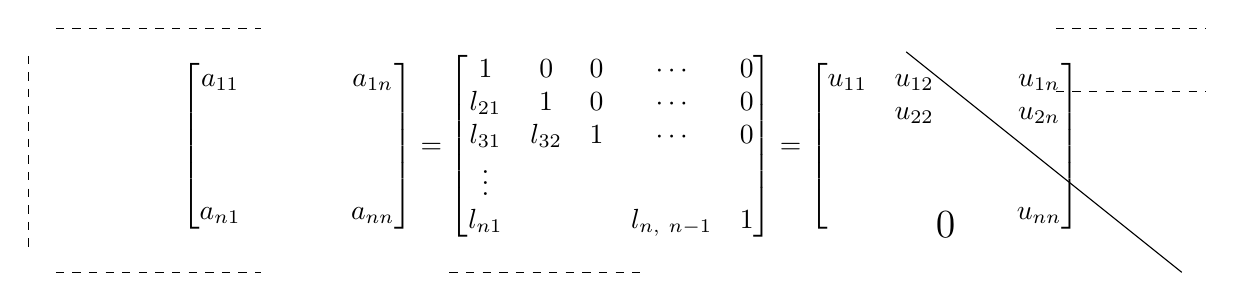
\begin{tikzpicture}
\node {$\begin{bmatrix}
a_{11} &  &  &  & a_{1n} \\ 
 &  &  &  &  \\ 
 &  &  &  &  \\ 
 &  &  &  &  \\ 
a_{n1} &  &  &  & a_{nn}
\end{bmatrix}=\begin{bmatrix}
1 & 0 & 0 & \cdots & 0 \\ 
l_{21} & 1 & 0 & \cdots & 0 \\ 
l_{31} & l_{32} & 1 & \cdots & 0 \\ 
\vdots &  &  &  &  \\ 
l_{n1} &  &  & l_{n,~n-1} & 1
\end{bmatrix}=\begin{bmatrix}
u_{11} & u_{12} &  &  & u_{1n} \\ 
 & u_{22} &  &  & u_{2n} \\ 
 &  &  &  &  \\ 
 &  &  &  &  \\ 
 &  &  &  & u_{nn}
\end{bmatrix} $};
\node at (4,-1) {\Large 0};
\draw[dashed] (-7.3,1.5) -- (-4.7,1.5);
\draw[dashed] (-7.65,1.15) -- (-7.65,-1.35);
\draw[dashed] (-7.3,-1.6) -- (-4.7,-1.6);
\draw[dashed] (-2.3,-1.6) -- (0.2,-1.6);
\draw[dashed] (5.4,1.5) -- (7.3,1.5);
\draw[dashed] (5.4,0.7) -- (7.3,0.7);
\draw (3.5, 1.2) -- (7,-1.6);
\end{tikzpicture}

De esta forma, el sistema $Ax=b$ se reescribe como $LUx=b$ y
llamando $z=Ux$ se llega a los sistemas

\hspace{1cm}$\left\lbrace\begin{array}{l}
Lz=b\\
Ux=z
\end{array}\right.$

que son dos sistemas fácilmente resolubles al ser $L$ y $U$
triangulares inferior y superior, respectivamente. Para el
cálculo del determinante de $A$, se tiene

\begin{center}
\fcolorbox{lightblue}{lightblue!10}{$|A|=|LU|=|L|\cdot|U|=1\cdot|U|=\prod_{j=1}^{n}u_{jj}$}
\end{center}
Volviendo al sistema
$Ax=b\xleftrightarrow{\hspace{1.5cm}}\left\lbrace\begin{array}{l}
Lz=b\\
Ux=z
\end{array}\right.$

Veamos cómo se resuelve un sistema triangular y el coste
computacional que lleva conflicto

$\begin{bmatrix}
u_{11} & u_{12} & \cdots & u_{2n} \\ 
0 & u_{22} & \cdots & u_{2n} \\ 
\vdots & \vdots & \ddots &  \\ 
0 & 0 & \cdots & u_{nn}
\end{bmatrix}\cdot\begin{bmatrix}
x_1\\
x_2\\
\vdots\\
x_n
\end{bmatrix}=\begin{bmatrix}
z_1\\
z_2\\
\vdots\\
z_n
\end{bmatrix}$

Se resuelven en cascada, de abajo hacia arriba.

$u_{nn}x_{n}\xrightarrow{\hspace{1.5cm}}x_{n}=\dfrac{z_{n}}{u_{nn}}$

$u_{n-1,~n-1}x_{n-1}+u_{n-1,~n}x_{n}=z_{n-1}\xrightarrow{\hspace{1.5cm}}x_{n-1}=\dfrac{x_{n-1}-u_{n-1,~n}\cdot
x_n}{u_{n-1,~n-1}}$

En general,
\begin{center}
\fcolorbox{lightblue}{lightblue!10}{$x_i=\dfrac{z_i-\displaystyle\sum_{j=i+1}^{n}u_{\imath\jmath  }x_{\jmath}}{u_{ii}}$}
\end{center}
Por tanto, el algoritmo es:

\hspace{1cm}$\left\lbrace\begin{array}{l}
x_{n}=\dfrac{z_{n}}{u_{nn}}\\
x_i=\dfrac{z_i-\displaystyle\sum_{j=i+1}^{n}u_{\imath\jmath  }x_{\jmath}}{u_{ii}}\end{array}\right.$

\textcolor{lightblue}{\underline{Análisis del coste
computacional}}

Consideremos el caso número 4.

$\left.\begin{array}{r}
u_{11}x_1+u_{12}x_2+u_{13}x_3+u_{14}x_4=z_1\\
u_{22}x_2+u_{23}x_3+u_{24}x_4=z_2\\
u_{33}x_3+u_{34}x_4=z_3\\
u_{44}x_4=z_4\\
\end{array}\right\rbrace$

$x_4=\dfrac{z_4}{u_{44}}$\hspace{1cm} 1 Operación

$x_3=\dfrac{z_3-u_{34}x_4}{u_{33}}$\hspace{1cm} 3 Operaciones

$x_2=\dfrac{z_2-u_{23x_3-u_{24}x_4}}{u_{22}}$\hspace{1cm} 5
Operaciones

$x_1=\dfrac{z_1-u_{12}x_2-u_{13}x_3-u_{14}x_4}{u_{11}}$\hspace{1cm}
7 Operaciones

En total, $16=4^2$ operaciones

Se observa que para calcular $x$; necesitamos
\fcolorbox{lightblue}{lightblue!10}{$2(n-i)+1$} operaciones.

Por tanto, el número total de operaciones es 

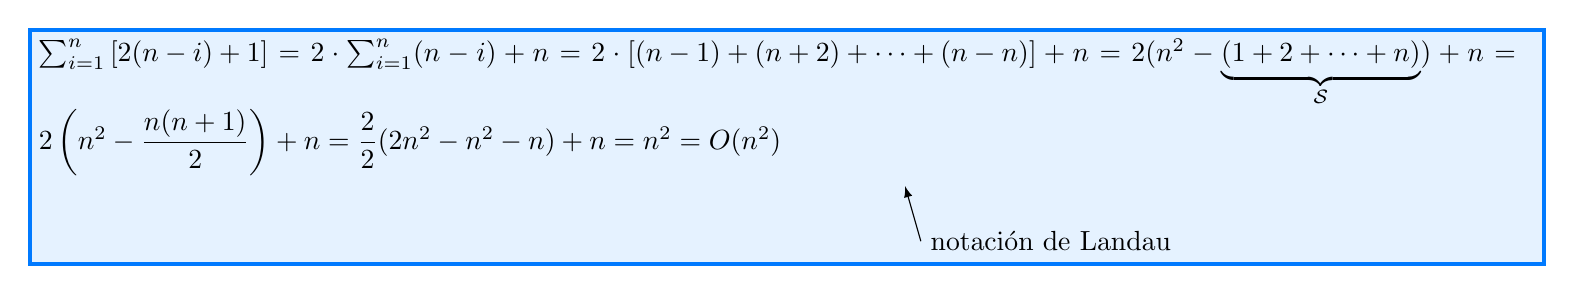
\begin{tikzpicture}
\node[draw=lightblue, fill=lightblue!10, rectangle, line
width=1.5pt, text width=19cm]
{$\sum_{i=1}^n\left[2(n-i)+1\right]=2\cdot\sum_{i=1}^n(n-i)+n=2\cdot\left[(n-1)+(n+2)+\cdots+(n-n)\right]+n=2(n^2-\underbrace{(1+2+\cdots+n)}_{\mathcal{S}})+n=2\left(n^2-\dfrac{n(n+1)}{2}\right)+n=\dfrac{2}{2}(2n^2-n^2-n)+n=n^2=O(n^2)$\vspace{1cm}};
\draw[latex-] (1.5,-0.5) -- (1.7,-1.2) node[right] {notación de
Landau};
\end{tikzpicture}

$\begin{array}{l}
\mathcal{S} = 1+2+\cdots+n\\
\mathcal{S} = n+n-1+\cdots+1\\
\rule{4.5cm}{0.4pt}\\
2\mathcal{S} = n\cdot(n+1)\longrightarrow
\mathcal{S}=\dfrac{n(n+1)}{2}
\end{array}$

\begin{itemize}[label=\color{red}\textbullet, leftmargin=*]
\item \color{lightblue} ¿Cómo se calculan $L$ y $U$ tales que
$A=LU$?
\end{itemize}
Haciendo eliminación Gaussiana. Veamos un ejemplo:

$A=\begin{bmatrix}
2 & -1 & 0 \\ 
-1 & 2 & -1 \\ 
0 & -1 & 2
\end{bmatrix}$ matriz de Toeplitz en dimensión 3.

$\begin{bmatrix}
2 & -1 & 0 \\ 
-1 & 2 & -1 \\ 
0 & -1 & 2
\end{bmatrix}\overset{F_2\rightarrow
F_2+\frac{1}{2}F_1}{\xrightarrow{\hspace{1.5cm}}}\begin{bmatrix}
2 & -1 & 0 \\ 
0 & \frac{3}{2} & -1 \\ 
0 & -1 & 2
\end{bmatrix}\overset{F_3\rightarrow
F_2+\frac{2}{3}F_2}{\xrightarrow{\hspace{1.5cm}}}\begin{bmatrix}
2 & -1 & 0 \\ 
0 & \frac{3}{2} & -1 \\ 
0 & 0 & \frac{4}{3}
\end{bmatrix} $

La matriz $U$ es 

$U=\begin{bmatrix}
2 & -1 & 0 \\ 
0 & \frac{3}{2} & -1 \\ 
0 & 0 & \frac{4}{3}
\end{bmatrix} $
\begin{itemize}[label=\color{red}\textbullet, leftmargin=*]
    \item \color{lightblue} ¿Donde está $L$?
\end{itemize}
Además de los pivotes, en la eliminación gaussiana juegan un
papel los llamados \textcolor{lightblue}{multiplicadores}.

Una vez conocemos el pivote de la fila $j$, y la entrada que se
desea eliminar en la fila $i$, el multiplicador $l_{\imath\jmath  }$ se
define como
\begin{center}
\fcolorbox{lightblue}{lightblue!10}{$l_{\imath\jmath  }=\dfrac{\text{entrada
a eliminar en la fila }i\text{-ésima}}{\text{pivote en la fila
}\jmath}$}
\end{center}
Así, en el ejemplo anterior:
\[l_{21}=\dfrac{-1}{2},~l_{31}=\dfrac{0}{2}=0,~l_{32}=\dfrac{-1}{\frac{3}{2}}?-\dfrac{2}{3}\]

La matriz $L$ es justo la matriz de multiplicadores en la
eliminación gaussiana. En nuestro caso: \[L=\begin{bmatrix}
1 & 0 & 0 \\ 
-\frac{1}{2} & 1 & 0 \\ 
0 & -\frac{2}{3} & 1
\end{bmatrix} \]
En efecto:
\[LU=\begin{bmatrix}
1 & 0 & 0 \\ 
-\frac{1}{2} & 1 & 0 \\ 
0 & -\frac{2}{3} & 1
\end{bmatrix}\cdot\begin{bmatrix}
2 & -1 & 0 \\ 
0 & \frac{3}{2} & -1 \\ 
0 & 0 & \frac{4}{3}
\end{bmatrix}=\begin{bmatrix}
2 & -1 & 0 \\ 
-1 & 2 & -1 \\ 
0 & -1 & 2
\end{bmatrix}=A\]
Veamos ahora una forma algorítmica de calcular la factorización
$LU$.

$\begin{array}{r}
\text{Sean }A=(a_{\imath\jmath  })\in M_{m\times n},~L=(l_{\imath\jmath  })\in
M_{m\times n}\\
U=(l_{\imath\jmath  })\in M_{m\times n}
\end{array}$

Entonces, si $A=LU$, se tiene:

\begin{center}
\fcolorbox{lightblue}{lightblue!10}{$a_{\imath\jmath  }=\sum_{k=1}^{n}l_{ik}u_{kj}$}
\end{center}

Como $l_{ik}=0$ si $k>i$ y $u_{kj}=0$ si $kj$, entonces podemos
distinguir dos casos:

\textcolor{lightblue}{Caso 1: $i>j\longrightarrow$}
$\min\{i,~j\}=j$

$a_{\imath\jmath  }=\sum_{k=1}^{\jmath}l_{ik}u_{kj}=l_{i1}u_{1j}+l_{i2}u_{2\jmath}+\cdots+l_{ii}u_{\imath\jmath  }$
y así:
$l_{\imath\jmath  }=\dfrac{a_{\imath\jmath  }-\displaystyle\sum_{k=1}^{\jmath-1}l_{ik}u_{kj}}{u_{jj}}$

\textcolor{lightblue}{Caso 2: $i\le j\longrightarrow$}
$\min\{i,~j\}=i$

$a_{\imath\jmath  }=\sum_{k=1}^{\jmath}l_{ik}u_{kj}=l_{i1}u_{1j}+l_{i2}u_{2\jmath}+\cdots+l_{ii}u_{\imath\jmath  }$
y así: $u_{\imath\jmath  }=a_{\imath\jmath  }-\sum_{k=1}^{\jmath-1}l_{ik}u_{kj}$ ya que
$l_{ii}=1$

Veamos cómo funciona este algoritmo para 

\[A=\begin{bmatrix}
2 & -1 & 0 \\ 
-1 & 2 & -1 \\ 
0 & -1 & 2
\end{bmatrix},~L=\begin{bmatrix}
1 & 0 & 0 \\ 
-\frac{1}{2} & 1 & 0 \\ 
0 & -\frac{2}{3} & 1
\end{bmatrix},~U=\begin{bmatrix}
2 & -1 & 0 \\ 
0 & \frac{3}{2} & -1 \\ 
0 & 0 & \frac{4}{3}
\end{bmatrix}\]

\underline{Primera fila de $U$:}

$u_{11}=a_{11}=2,~u_{12}=a_{12}=-1,~u_{13}=a_{13}=0$

\underline{Primera columna de $L$:}

$l_{11}=1,~l_{21}=\frac{a_{21}}{u_{11}}=-\frac{1}{2},~l_{31}=\frac{a_{31}}{u_{11}}=\frac{0}{2}=0$

\underline{Segunda fila de $U$:}

$u_{22}=a_{22}-\sum_{k=1}^{1}l_{2k}u_{k2}=a_{22}-l_{21}u_{12}=2-\frac{1}{2}(-1)=\frac{3}{2}$

$u_{23}=a_{23}-\sum_{k=1}^{1}l_{2k}u_{k3}=a_{23}-l_{21}u_{13}=-1-\left(-\frac{1}{2}\right)\cdot
0=-1$

\underline{Segunda columna de $L$:}

$l_{32}=\dfrac{a_{32}-\displaystyle\sum_{k=1}l_{3k}u_{k2}}{u_{22}}=\dfrac{-1-(0)}{\frac{3}{2}}=-\dfrac{2}{3}$

\underline{Tercera fila de $U$}

$u_{33}=a_{33}-\sum_{k=1}^{2}l_{2k}u_{k3}=2-(l_{31}u_{13}+l_{32}u_{23})=2-\left(0+0-\dfrac{2}{3}\cdot(-1)\right)=2-\dfrac{2}{3}=\dfrac{4}{3}$
\begin{itemize}[label=\color{red}\textbullet, leftmargin=*]
    \item \color{lightblue} Nota 1:
\end{itemize}
Se puede probar que el coste computacional de resolver un
sistema lineal $Ax=b$ mediante descomposición $LU$ es
$\dfrac{n^3+3n^2-1}{3}$ siendo $n$ el tamaño de la matriz $A$.
\begin{itemize}[label=\color{red}\textbullet, leftmargin=*]
    \item \color{lightblue} Nota 2:
\end{itemize}
Realizando, si fuera necesario, permutaciones de filas (para
llevar filas nulas al final) es fácil observar que toda matriz
$A\in M_{m\times n}(\mathbb{K})$ admite una factorización $PLU$,
es decir, \begin{center}
\fcolorbox{lightblue}{lightblue!10}{$PA=LU$}
\end{center}donde:

\begin{itemize}
\item $P\in M_{m\times n}(\mathbb{K})$ es una matriz de
permutación.
\item $L\in M_{m\times n}(\mathbb{K})$ triangular inferior con
1s en la diagonal.
\item $U\in M_{m\times n}(\mathbb{K})$ triangular superior.
\end{itemize}
Volviendo a la factorización:

$$\underbrace{\begin{bmatrix}
2 & -1 & 0 \\ 
-1 & 2 & -1 \\ 
0 & -1 & 2
\end{bmatrix} }_A=\underbrace{\begin{bmatrix}
1 &  &  \\ 
-\dfrac{1}{2} & 1 &  \\ 
0 & -\dfrac{2}{3} & 1
\end{bmatrix} }_L\cdot\underbrace{\begin{bmatrix}
2 & -1 & 0 \\ 
 & \dfrac{3}{2} & -1 \\ 
 &  & \dfrac{4}{3}
\end{bmatrix} }_U$$
se observa que el carácter simétrico de la matriz $A$ se pierde
en la factorización $LU$. Esta simetría se puede superar
separando los pivotes (entradas en diagonal de $U$) en una
matriz diagonal $D$ y dividiendo cada fila de $U$ por su
correspondiente pivote. Se obtiene así:

\[\underbrace{\begin{bmatrix}
2 & -1 & 0 \\ 
-1 & 2 & -1 \\ 
0 & -1 & 2
\end{bmatrix} }_A=\underbrace{\begin{bmatrix}
1 &  &  \\ 
-\dfrac{1}{2} & 1 &  \\ 
0 & -\dfrac{2}{3} & 1
\end{bmatrix} }_L\cdot\underbrace{\begin{bmatrix}
2 &  &  \\ 
 & \dfrac{3}{2} &  \\ 
 &  & \dfrac{4}{3}
\end{bmatrix} }_U\cdot\underbrace{\begin{bmatrix}
1 & -\dfrac{1}{2} & 0 \\ 
 & 1 & -\dfrac{2}{3} \\ 
 &  & 1
\end{bmatrix} }_{L^T}\]



En resumen:\begin{center}
\fcolorbox{lightblue}{lightblue!10}{$A=LDL^{T}$}
\end{center}factorización llamada Cholesky.

Además, $D$ se puede factorizar como \[D=\begin{bmatrix}
2 &  &  \\ 
 & \dfrac{3}{2} &  \\ 
 &  & \dfrac{4}{3}
\end{bmatrix}=\underbrace{\begin{bmatrix}
\sqrt{2} &  &  \\ 
 & \sqrt{\dfrac{3}{2}} &  \\ 
 &  & \dfrac{2}{\sqrt{3}}
\end{bmatrix} }_{\sqrt{D}}\cdot\underbrace{\begin{bmatrix}
\sqrt{2} &  &  \\ 
 & \sqrt{\dfrac{3}{2}} &  \\ 
 &  & \dfrac{2}{\sqrt{3}}
\end{bmatrix} }_{\sqrt{D}}\]
se llega así:
\[\underbrace{\begin{bmatrix}
1 &  &  \\ 
-\dfrac{1}{2} & 1 &  \\ 
0 & -\dfrac{2}{3} & 1
\end{bmatrix} }_L\cdot\underbrace{\begin{bmatrix}
\sqrt{2} &  &  \\ 
 & \sqrt{\dfrac{3}{2}} &  \\ 
 &  & \dfrac{2}{\sqrt{3}}
\end{bmatrix} }_{\sqrt{D}}=\underbrace{\begin{bmatrix}
\sqrt{2} &  &  \\ 
-\dfrac{\sqrt{2}}{2} & \sqrt{\dfrac{3}{22}} &  \\ 
0 & -\dfrac{2}{3}\sqrt{\dfrac{3}{2}} & \dfrac{2}{\sqrt{3}}
\end{bmatrix} }_{\begin{array}{c}
\tilde{L}\\
\text{Columnas de }L\times\sqrt{\text{pivotes}}
\end{array}}\]

\[\underbrace{\begin{bmatrix}
\sqrt{2} &  &  \\ 
 & \sqrt{\dfrac{3}{2}} &  \\ 
 &  & \dfrac{2}{\sqrt{3}}
\end{bmatrix} }_{\sqrt{D}}\cdot\underbrace{\begin{bmatrix}
1 & -\dfrac{1}{2} & 0 \\ 
 & 1 & -\dfrac{2}{3} \\ 
 &  & 1
\end{bmatrix} }_{L^T}=\underbrace{\begin{bmatrix}
\sqrt{2} & -\dfrac{\sqrt{2}}{2} & 0 \\ 
 & \sqrt{\dfrac{3}{2}} & -\dfrac{2}{3}\sqrt{\dfrac{3}{2}} \\ 
 &  & \dfrac{2}{\sqrt{3}}
\end{bmatrix} }_{\begin{array}{c}
\tilde{L}^T\\
\sqrt{\text{pivotes}}\times\text{ filas de }L^T
\end{array}}\]

Con lo que obtenemos una nueva forma de la factorización
Cholesky, a saber, $A=\tilde{L}\cdot\tilde{L}^T$
\begin{itemize}[label=\color{red}\textbullet, leftmargin=*]
    \item \color{lightblue} Nota (Importante)
\end{itemize}
Nótese que procedimiento ha influido porque los pivotes han
salido positivos. Si hubieran salido negativos no lo hubiéramos
podido hacer. Los pivotes son siempre positivos para una clase
especial (pero que aparecen con muchísima frecuencia en
Ingeniería) de matrices llamadas definidas positivas.
\begin{itemize}[label=\color{red}\textbullet, leftmargin=*]
    \item \color{lightblue} Definición
\end{itemize}
Una matriz simétrica $A\in M_{n}(\mathbb{R})$ se dice
\textcolor{lightblue}{definida positiva} si $x^TAx>0~\forall
x\neq0$. Más adelante veremos una caracterización de este tipo
de matrices.
\begin{itemize}[label=\color{red}\textbullet, leftmargin=*]
    \item \color{lightblue} Nota (Coste computacional)
\end{itemize}
Para resolver un sistema $Ax=b$, con $A$ simétrica y definida
positiva mediante Cholesky hemos de resolver los sistemas
triangulares\begin{center}
\fcolorbox{lightblue}{lightblue!10}{$L_y=b,~L^Tx=y$}
\end{center}
Para dar una respuesta satisfactoria, necesitamos introducir
\textcolor{lightblue}{normas de matrices}

Sea $A\in M_{m\times n}(\mathbb{K})$. Se define la norma de $A$,
como $\|A\|=\max_{x\neq0\longrightarrow}\dfrac{\|Ax\|}{\|x\|}$

Obviamente se tiene que \begin{center}
\fcolorbox{lightblue}{lightblue!10}{$\dfrac{\|Ax\|}{\|x\|}\le\|A\|$}
\end{center}
y así: \fcolorbox{lightblue}{lightblue!10}{$\|Ax\|\le\|A\|\cdot\|x\|$}

La \textcolor{lightblue}{llave} para la estabilidad de sistemas lineales está en el concepto de número de condicionamiento de una matriz.

\begin{itemize}[label=\color{red}\textbullet, leftmargin=*]
    \item \color{lightblue} Definición
\end{itemize}

Dada $A$ invertible, se define el número de condicionamiento como \begin{center}
\fcolorbox{lightblue}{lightblue!10}{$\mathrm{c}(A)=\|A\|\cdot\|A^{-1}\|$}
\end{center}
El coste computacional total es del orden de $\dfrac{n^3}{6}$, justo la mitad que la factorización $LU$.

Por eso, para este tipo de matrices simétricas y definidas positivas se ha de usar Cholesky. Nótese que en la factorización $LU$ hemos de calcular $L$ y $U$ mientras que en Choleski sólo $L$. Por eso el coste computacional es la mitad.

\textcolor{lightblue}{\underline{Análisis de errores}}

Analizamos a continuación la llamada cuestión de la \textcolor{lightblue}{estabilidad} en la resolución de un sistema lineal. La situación es como sigue:
\begin{itemize}
\item Para el sistema \fcolorbox{lightblue}{lightblue!10}{$Ax=b$}, si $b$ se cambia por $b+\Delta b$, debido por ejemplo a errores de representación o redondeo, entonces en lugar de $x$ tendremos $x+\Delta x$
\end{itemize}
\begin{itemize}[label=\color{red}\textbullet, leftmargin=*]
    \item \color{lightblue} ¿Cómo podemos estimar o controlar $\Delta x$ en función de $\Delta b$?
\end{itemize}
Esta es la pregunta de la \textcolor{lightblue}{estabilidad}.
\begin{itemize}[label=\color{red}\textbullet, leftmargin=*]
    \item \color{lightblue}Nota
\end{itemize}
Como puede intuirse, no es fácil calcular el número de condicionamiento de una matriz. Dejamos para más adelante esta cuestión. La resolveremos vía valores propios y valores singulares al final de este curso.

Ya estamos en condiciones de dar respuesta a la cuestión anterior sobre control de error en la resolución de sistemas lineales.

Sea $Ax=b$ un sistema compatible determinado. Si se perturba el término independiente de $b$ por $\Delta b$, la nueva solución $x+\Delta x$\begin{center}
\fcolorbox{lightblue}{lightblue!10}{$A(x+\Delta x)=b+\Delta b$}\end{center} de modo que el error $\Delta x$ es solución de \begin{center}
\fcolorbox{lightblue}{lightblue!10}{$A(\Delta x)=\Delta b,$} \end{center}es decir, \begin{center}
\fcolorbox{lightblue}{lightblue!10}{$\Delta x=A^{-1}(\Delta b)$} \end{center}y así \begin{center}
\fcolorbox{lightblue}{lightblue!10}{$\|\Delta x\|=\|A^{-1}(\Delta b)\|\le\|A^{-1}\|\cdot\|\Delta b\|,$}\end{center} lo que nos da una cota del \textcolor{lightblue}{error absoluto} $\Delta x$.

Más importante que el error absoluto es el \textcolor{lightblue}{relativo}, el cual estimamos a continuación:
\begin{itemize}
\item Dado que $Ax=b$, se tiene que $\|Ax\|=\|b\|$
\end{itemize}
Así:
\begin{center}
\fcolorbox{lightblue}{lightblue!10}{$\|\Delta x\|\le\|A^{-1}\|\cdot\|\Delta b\|=\|A^{-1}\|\cdot\|\Delta b\|\cdot\overbrace{\dfrac{\|Ax\|}{\|b\|}}^{1}\le\|A^{-1}\|\cdot\|A\|\cdot\|x\|\cdot\dfrac{\|\Delta b\|}{\|b\|}$}
\end{center}de donde \begin{center}
\fcolorbox{lightblue}{lightblue!10}{$\dfrac{\|\Delta x\|}{\|x\|}\le\|A\|\cdot\|A^{-1}\|\cdot\dfrac{\|\Delta b\|}{\|b\|}=\mathrm{c}(A)\cdot\dfrac{\|\Delta b\|}{\|b\|}$}
\end{center}

Es decir, el \textcolor{lightblue}{número de condicionamiento} controla la propagación del error relativo del término independiente a la solución.

\begin{itemize}[label=\color{red}\textbullet, leftmargin=*]
    \item \color{lightblue}Nota:
\end{itemize}
Se puede probar que si el error se produce en $A$, (cosa habitual cuando $A$ se factoriza en forma $LU$ o Cholesky), entonces también el \textcolor{lightblue}{número de condicionamiento} controla la propagación del error.

En resumen, si $\mathrm{c}(A)$ está mal condicionada y la solución $x$ puede ser muy sensible con respecto a pequeños errores en la matriz $A$ y/o en el término independiente $b$.

Por eso hemos de precisar \textcolor{lightblue}{qué entendemos por un número de condicionamiento grande}. No hay un teorema matemático que de respuesta a esta pregunta, pero sí resultados de experimentos numéricos que sugieren la siguiente regla.
\begin{center}
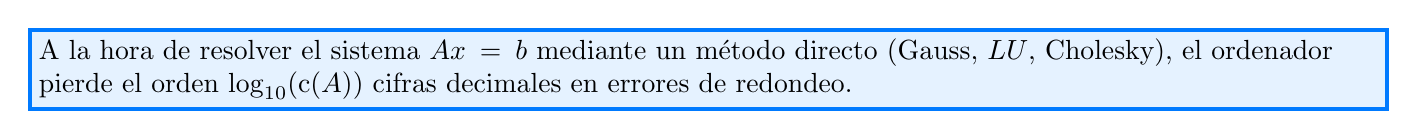
\begin{tikzpicture}
\node[draw=lightblue, fill=lightblue!10, line width=1.5, text width=17cm, rectangle] {A la hora de resolver el sistema $Ax=b$ mediante un método directo (Gauss, $LU$, Cholesky), el ordenador pierde el orden $\log_{10}(\mathrm{c}(A))$ cifras decimales en errores de redondeo.};
\end{tikzpicture}
\end{center}
Para finalizar, veamos un ejemplo concreto.
\begin{itemize}[label=\color{red}\textbullet, leftmargin=*]
    \item \color{lightblue} Ejemplo
\end{itemize}
$A=\begin{bmatrix}
1 & 7 \\ 
0 & 1
\end{bmatrix},~b=\begin{bmatrix}
7 \\ 
1
\end{bmatrix}$

Consideramos el sistema $Ax=b$

$\begin{bmatrix}
1 & 7 \\ 
0 & 1
\end{bmatrix}\cdot\begin{bmatrix}
x_{1}\\
x_{2}
\end{bmatrix}=\begin{bmatrix}
7 \\ 
1
\end{bmatrix}$

$\left.\begin{array}{r}
x_{1}+7x_{2}=7\\
x_{2}=1
\end{array}\right\rbrace$\fbox{$x_{1}=0,~x_2=1$}

Supongamos que $b$ se perturba por $\Delta b=\begin{bmatrix}
0\\
0.1
\end{bmatrix}$.

El error en $x$, denotado $\Delta x$, es solución de $A(\Delta x)=\Delta b$;

\[\begin{bmatrix}
1 & 7 \\ 
0 & 1
\end{bmatrix}\cdot\begin{bmatrix}
\Delta x_{1}\\
\Delta x_{2}
\end{bmatrix}=\begin{bmatrix}
0 \\ 
0.1
\end{bmatrix}\]
$\left.\begin{array}{r}
\Delta x_{1}+7\Delta x_{2}=0\\
\Delta x_{2}=0.1
\end{array}\right\rbrace\longrightarrow\Delta x_{1}=-7\Delta x_{2}=-0.7$

\fbox{$\Delta x_{1}=-0.7,~\Delta x_{2}=0.1$}

El error relativo en $x$ es:\begin{center}
\fcolorbox{lightblue}{lightblue!10}{$\dfrac{\|\Delta x\|}{\|x\|}=\dfrac{\sqrt{(-0.7)^2+0.1^2}}{\sqrt{0^2+1^2}}=0.1\sqrt{50}$}
\end{center}
El error absoluto en $b$ es:\begin{center}
\fcolorbox{lightblue}{lightblue!10}{$\dfrac{\|\Delta b\|}{\|b\|}=\dfrac{0^2+0.1^2}{\sqrt{7^2+1^2}}=\dfrac{0.1}{\sqrt{50}}$}\end{center}
Por tanto, \begin{center}
\fcolorbox{lightblue}{lightblue!10}{$\dfrac{\|\Delta x\|}{\|x\|}=0.1\sqrt{50}=\sqrt{50}\cdot\sqrt{50}\dfrac{0.1}{\sqrt{50}}=50\dfrac{0.1}{\sqrt{50}}=\dfrac{\|\Delta b\|}{\|b\|}$}
\end{center} es decir, el error de salida es \textcolor{lightblue}{50 veces} mayor que en la entrada.

Si calculamos, con Python, el número de condicionamiento de $A$, nos devuelve $\mathrm{c}(A)=51$. Para la norma de Frobenius observamos pues que el número de condicionamiento de una estimación bastante precisa de la propagación del error

\textcolor{lightblue}{\underline{Métodos iterativos para la resolución de sistemas lineales}}
\begin{itemize}[label=\color{red}\textbullet, leftmargin=*]
    \item \color{lightblue} ¿Qué hacer si $\mathrm{c}(A)>>1$?
\end{itemize}
En lugar de resolver el sistema $Ax=b$, resolveremos el sistema equivalente \begin{center}
\fcolorbox{lightblue}{lightblue!10}{$\mathrm{c}(C^{-1}\cdot Ax)=C^{-1}\cdot b$}
\end{center} de modo que la matriz invertible $C$ haga que \begin{center}
\fcolorbox{lightblue}{lightblue!10}{$\mathrm{c}(C^{-1}A)<<\mathrm{c}(A)$}
\end{center}
\begin{itemize}[label=\color{red}\textbullet, leftmargin=*]
    \item \color{lightblue}¿Cómo elegir $C$?
\end{itemize}
La primera opción sería tomar $C=A$. En este caso, $C^{-1}\cdot A=A^{-1}\cdot A=I$, cuyo número de condicionamiento es 1.

Sin embargo, calcular $A^{-1}$ es igual de costoso que resolver $Ax=b$.

El intento de tomar $C=A$ no es útil pero nos sugiere que la matriz $C$ ha de ser \textcolor{lightblue}{próxima} a $A$.

Otras dos opciones más prácticas son:
\begin{enumerate}[label=\arabic*)]
    \item Si $A$ no tiene ceros en la diagonal,  tomamos $C=\diag(a_{11},a_{12},\hdots,a_{nn})$.
    
    \underline{Ejemplo}
    
    $A=\begin{bmatrix}
    	8 & -2\\
    	-2 & 50
	\end{bmatrix}  $\hspace{1cm} Python $\longrightarrow~\mathrm{c}(A)=6.3371$
	
	$C=\begin{bmatrix}
	8 & 0 \\ 
	0 & 50
	\end{bmatrix}\hspace{1cm}C^{-1}=\begin{bmatrix}
	\frac{1}{8} & 0 \\ 
	0 & \frac{1}{50}
	\end{bmatrix} $ 
	
	$\mathrm{c}(C^{-1}\cdot A)=1.3370$
	\item Tomar $C^{-1}=\mathrm{p}(A)$, un polinomio de $A$ que resulta de \textcolor{lightblue}{truncar} la serie de $A^{-1}$.
	
	Es decir, \begin{center}
	\fcolorbox{lightblue}{lightblue!10}{$A^{-1}=I-(I-A)^{-1}=\dfrac{1}{I-(I-A)}=I+(I-A)+(I+A)^2+\cdots$}
	\end{center} lo cual converge si $\|I-A\|<1$
\end{enumerate}
Por tanto, \begin{center}
\fcolorbox{lightblue}{lightblue!10}{$C^{-1}=I+\sum_{k=1}^{N}(I-A)^{K}$}
\end{center}
Teniendo en mente la idea de usar una matriz próxima a $A$ para reducir el número de condicionamiento de la matriz del nuevo sistema se introducen los \textcolor{lightblue}{métodos iterativos} del siguiente modo:
\begin{itemize}
\item Dado que $Ax=b$, para toda matriz $P$, que a partir de ahora llamaremos precondicionador, se tiene que \begin{center}
\fcolorbox{lightblue}{lightblue!10}{$Px=(P-A)x+b$}
\end{center}
\end{itemize}
Esta descomposición sugiere un algoritmo iterativo en el que a partir de $X_{k}$ calculamos $x_{k+1}$ siguiendo el algoritmo.

\fcolorbox{lightblue}{lightblue!10}{$Px_{k+1}=(P-A)x_{k}+b$}

El éxito de este algoritmo está garantizado si se cumple:
\begin{enumerate}[label=\arabic*)]
    \item $x_{k+1}$ se calcula fácilmente a partir de $x_{k}$.
    \item Los errores $e_{k}=x-x_{k}$ se aproximan a cero, es decir, el algoritmo es convergente.
\end{enumerate}
Veamos qué ha de suceder para que el algoritmo sea convergente:

$\begin{array}{ll}
\text{Tenemos: } & Px_{k+1}=(P-A)x_{k}+b\\
 & Px=(P-A)x+b
\end{array}$

$\begin{array}{ll}
\text{Si restamos: } & P(x-x_{k+1})=(P-A)(x-x_{k})\\
 & Pe_{k+1}=(P-A)\cdot e_{k}
\end{array}$

de donde suponiendo que $P$ es invertible: 
\begin{center}
\fcolorbox{lightblue}{lightblue!10}{$e_{k+1}=P^{-1}(P-A)e_{k}=\underbrace{(I-P^{-1}\cdot A)}_{M}e_{k}$}
\end{center}

Repitiendo el proceso y calculando normas:\begin{center}
\fcolorbox{lightblue}{lightblue!10}{$\|e_{k+1}\|=\|M_{ek}\|=\|M\|\cdot\|e_k\|\le\|M\|\cdot\|M\|\cdot\|e_{k-1}\|=\|M\|^2\cdot\|e_{k-1}\|\le\cdots_{k+1}\le\|M\|\cdot\|e_0\|$}
\end{center} lo que significa que $\|e_{k+1}\|\underset{k\rightarrow +\infty}{\longrightarrow 0}$ si $\|M\|<1$.

La pregunta del millón sigue siendo:
\begin{itemize}[label=\color{red}\textbullet, leftmargin=*]
    \item \color{lightblue} ¿Cómo elegir $P$?
\end{itemize}
Jacobi propuso tomar $P=D$, la parte diagonal de $A$. Esto conduce al llamado método de Jacobi. Esta opción es simple pero lenta.

En el lado opuesto, el método de Gauss-Seidel propone tomar como $P$ una matriz más próxima a $A$. En concreto, partimos de la descomposición \fcolorbox{lightblue}{lightblue!10}{$A=L+D+U$}.

\begin{center}
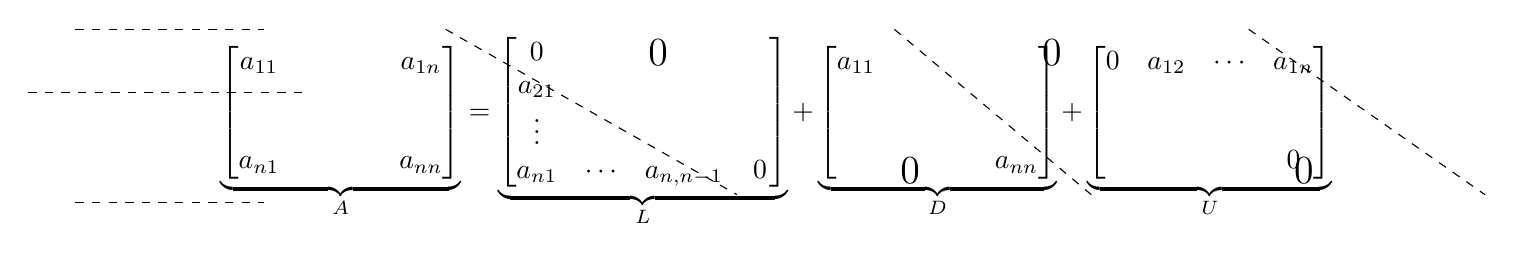
\begin{tikzpicture}
\node {$\underbrace{\begin{bmatrix}
a_{11} & ~~ & ~~ & a_{1n} \\ 
 &  &  &  \\ 
 &  &  &  \\ 
a_{n1} &  &  & a_{nn}
\end{bmatrix} }_{A}=\underbrace{\begin{bmatrix}
0 & ~~ & ~~ & ~~ \\ 
a_{21} &  &  &  \\ 
\vdots &  &  &  \\ 
a_{n1} & \cdots & a_{n,n-1} & 0
\end{bmatrix}}_{L}+\underbrace{\begin{bmatrix}
a_{11} & ~~ & ~~ &  \\ 
 &  &  &  \\ 
 &  &  &  \\ 
 &  &  & a_{nn}
\end{bmatrix} }_{D}+\underbrace{\begin{bmatrix}
0 & a_{12} & \cdots & a_{1n} \\ 
 &  &  &  \\ 
 &  &  &  \\ 
 &  &  & 0
\end{bmatrix} }_{U}$};
\draw[dashed] (-8.9,1.3) -- (-6.5,1.3);
\draw[dashed] (-9.5,0.5) -- (-6,0.5);
\draw[dashed] (-8.9,-0.9) -- (-6.5,-0.9);
\draw[dashed] (-4.2,1.3) -- (-0.5,-0.8);
\draw[dashed] (1.5,1.3) -- (4,-0.8);
\draw[dashed] (6,1.3) -- (9,-0.8);
\node at (-1.5,1) {\Large 0};
\node at (3.5,1) {\Large 0};
\node at (1.7,-0.5) {\Large 0};
\node at (6.7,-0.5) {\Large 0};
\end{tikzpicture}
\end{center}
En el método de Gauss-Seidel se toma $P=D+L$ de modo que el algoritmo \begin{center}
\fcolorbox{lightblue}{lightblue!10}{$Px_{k+1}=-Ux_{k}+b,~P=D+L$}
\end{center}
\underline{Ejemplo:} Aplicado al caso de la matriz $A=k_4$
\[k_4=\begin{bmatrix}
2 & -1 & 0 & 0 \\ 
-1 & 2 & -1 & 0 \\ 
0 & -1 & 2 & -1 \\ 
0 & 0 & -1 & 2
\end{bmatrix},~P=L+D=\begin{bmatrix}
2 & 0 & 0 & 0 \\ 
-1 & 2 & 0 & 0 \\ 
0 & -1 & 2 & 0 \\ 
0 & 0 & -1 & 2
\end{bmatrix}, ~U=\begin{bmatrix}
0 & -1 & 0 & 0 \\ 
0 & 0 & -1 & 0 \\ 
0 & 0 & 0 & -1 \\ 
0 & 0 & 0 & 0
\end{bmatrix} \]
El algoritmo queda: 
\[-1\cdot\begin{bmatrix}
0 \\ 
x_1 \\ 
x_2 \\ 
x_3
\end{bmatrix}_{\mathrm{new}}+2\begin{bmatrix}
x_1 \\ 
x_2 \\ 
x_3 \\ 
x_4
\end{bmatrix}_{\mathrm{new}}=\begin{bmatrix}
x_2 \\ 
x_3 \\ 
x_4
\end{bmatrix}_{\mathrm{old}}+\begin{bmatrix}
b_1 \\ 
b_2 \\ 
b_3 \\ 
b_4
\end{bmatrix} \]
\begin{itemize}[label=\color{red}\textbullet, leftmargin=*]
    \item \color{lightblue} ¿Cuándo tenemos garantizada la convergencia en este método?
\end{itemize}
Para el caso de las llamadas \textcolor{lightblue}{matrices diagonal dominantes}.
\begin{itemize}[label=\color{red}\textbullet, leftmargin=*]
    \item \color{lightblue} Definición
\end{itemize}
Una matriz $A=(a_{\imath\jmath  })$ se dice estrictamente diagonal dominante si para cada fila $i$ se cumple\begin{center}
\fcolorbox{lightblue}{lightblue!10}{$|a_{\imath\jmath  }|>\sum_{\begin{array}{c}
j=1\\
i\neq j
\end{array}}^{n}|a_{\imath\jmath  }|$}
\end{center}
\underline{Ejemplo}

$A=\begin{bmatrix}
2 & -1 & 0 \\ 
-1 & 4 & 2 \\ 
0 & 2 & 3
\end{bmatrix}\begin{array}{l}
|a_{11}|=2>1\\
|a_{22}|=4>2+1=3\\
|a_{33}|=3>2
\end{array}$
\begin{itemize}[label=\color{red}\textbullet, leftmargin=*]
    \item \color{lightblue}Teorema
\end{itemize}
Supongamos que $A$ es estrictamente diagonal dominante. Entonces, los métodos de Jacobi y Gauss-Seidel son convergentes.

\newpage
\section{Subespacios Vectoriales}
\textcolor{lightblue}{\underline{Subespacios vectoriales}}
\begin{itemize}[label=\color{red}\textbullet, leftmargin=*]
    \item \color{lightblue}Definición
\end{itemize}
Un subespacio (vectorial) de $\mathbb{K}^n$ es un subconjunto de $W$ de $\mathbb{K}^n$ que verifica:
\begin{enumerate}[label=\arabic*)]
    \item Si $w,w'\in W\longrightarrow w+w'\in W$.
    \item Si $w\in W$ y $\alpha\in\mathbb{K}\longrightarrow\alpha w\in W$.
\end{enumerate}
\underline{Nota:} Nótese que el vector 0 siempre pertenece a todo subespacio vectorial $W$. En efecto: dado $w\in W$, se tiene que $-1\cdot w=-w\in W$. Ademas $w+(-w)=0\in W$.

\underline{Ejemplo 1}

Sean $A\in M_{m\times n}(\mathbb{K})$ y $W$ el conjunto de soluciones del sistema $Ax=0$. Entonces, $W$ es un subespacio vectorial. En efecto: Si $w,w'\in W$, entonces $Aw=0$ y $Aw'=0$. Por tanto, $A(w+w')=Aw+Aw'=0+0=0$, lo que implica que $w+w'\in W$. El subespacio $W$ anterior se llama núcleo de $A$ y se denota $\mathrm{Nuc}(A)$.

\underline{Ejemplo 2}

Sea $\{u_{1},u_{2},\hdots,u_m\}$ un conjunto de vectores de $\mathbb{K}^n$.

Denotemos por $<u_1,u_2,\hdots,u_m>$ el conjunto formado por todas las combinaciones lineales de $\{u_{1},u_{2},\hdots,u_m\}$, es decir \begin{center}
\fcolorbox{lightblue}{lightblue!10}{$<u_{1},u_2,\hdots,u_m>=\left\lbrace w=\sum_{i=1}^m\alpha_iw_i,~\alpha_i\in\mathbb{K}\right\rbrace$}
\end{center}
Es fácil comprobar que $<u_1,u_2,\hdots,u_m>$ es un subespacio vectorial de $\mathbb{K}^n$. Este subespacio se llama \textcolor{lightblue}{subespacio generado} por   $\{u_{1},u_{2},\hdots,u_m\}$, y al conjunto de vectores, $\{u_{1},u_{2},\hdots,u_m\}$ se le llama \textcolor{lightblue}{conjunto generador}.
\begin{itemize}[label=\color{red}\textbullet, leftmargin=*]
    \item \color{lightblue} Definición (Base de un subespacio vectorial)
\end{itemize}
Sean $W$ un subconjunto vectorial de $\mathbb{K}^n$ y $B=\{u_{1},u_{2},\hdots,u_m\}$ un conjunto de vectores. Se dice que $B$ es una base de $W$ si se cumple:
\begin{enumerate}[label=\arabic*)]
    \item $W=<u_1,u_2,\hdots,u_m>$
    \item $\{u_{1},u_{2},\hdots,u_m\}$ son linealmente independientes.
\end{enumerate}
\underline{Ejemplo 1}

Sea $W=\mathbb{K}^n$. Entonces los vectores \[B=\{u_{1}=(1,0,\hdots,0),u_{2}=(0,1,0,\hdots,0),\hdots,u_n=(0,\hdots,0,1)\}\] 
Son una base de $W$. En efecto:
\begin{enumerate}[label=\arabic*)]
    \item $B$ es un conjunto generador ya que si $v=(v_1,\hdots,v_n)\in \mathbb{K}^n$, entonces \begin{center}
    \fcolorbox{lightblue}{lightblue!10}{$v=\sum_{i=1}^nv_iu_i$}
    \end{center}
    \item $B$ es literalmente independiente: \begin{center}
    \fcolorbox{lightblue}{lightblue!10}{$\sum\alpha_1u_i=0\longleftrightarrow(\alpha_1,\alpha_2,\hdots,\alpha_n)=(0,\hdots,0)\longrightarrow\alpha_i=0~~\forall~1\le i\le n$}
    \end{center}
\end{enumerate}
\underline{Ejemplo 2}
Sean 

$A=\begin{bmatrix}
1 & -1 & 1 \\ 
1 & 1 & 1
\end{bmatrix}$

y $W=\mathrm{nuc}(A)$, es decir, $W$ está formado por las soluciones del sistema \[Ax=0\longleftrightarrow\begin{bmatrix}
1 & -1 & 1 \\ 
1 & 1 & 1
\end{bmatrix}\cdot\begin{bmatrix}
x_{1}\\
x_2\\
x_3
\end{bmatrix}=[0,0]\qquad\left.\begin{array}{r}
x_1-x_2+x_3=0\\
x_1+x_2+x_3=0
\end{array}\right\rbrace \]
Como $\mathrm{rango}(A)=2$ se trata de un sistema compatible indeterminado. La solución depende de un parámetro. Tomamos $x_3=\lambda$:

$\left.\begin{array}{r}
x_1-x_2=-\lambda\\
x_1+x_2=-\lambda
\end{array}\right\rbrace\longrightarrow\begin{array}{l}
2x_1=-2\lambda\\
x_1=-\lambda\\
x_2=-\lambda-x_1=-\lambda-(-\lambda)=0
\end{array} $

$\left.\begin{array}{r}
x_1=-\lambda\\
x_2=0\\
x_3=\lambda
\end{array}\right\rbrace(x_1,x_2,x_3)=\lambda(-1,0,1)$

$B=\left\lbrace(-1,0,1)\right\rbrace$ es una base de $W$.
\begin{itemize}[label=\color{red}\textbullet, leftmargin=*]
    \item \color{lightblue} Teorema (de la base)
\end{itemize}
Sea $W$ un subespacio vectorial de $\mathbb{K}^n$. Entonces todas las bases de $W$ tienen el mismo número de elementos. A este número se le llama dimensión de $W$ y se denota $\mathrm{dim}(W)$.

\textcolor{lightblue}{\underline{Subespacios vectoriales y matrices}}

\begin{itemize}[label=\color{red}\textbullet, leftmargin=*]
    \item \color{lightblue}Subespacios asociados a una matriz. Rango
\end{itemize}
Dada $A\in M_{m\times n}(\mathbb{K})$, se definen los siguientes subespacios asociados a $A$:
\begin{enumerate}[label=\arabic*)]
\item $\mathrm{Col}(A)=$ subespacio generados por las columnas de $A$.
\item $\mathrm{Fil}(A)=$ subespacio generados por las filas de $A$.
\item $\mathrm{Nuc}(A)=$ subespacio generados por las soluciones de $Ax=0$.
\begin{itemize}
\item[$\longrightarrow$] Núcleo por la izquierda: subespacio generados por las soluciones de $x^TA=0$.
\end{itemize}
\end{enumerate}
\begin{itemize}[leftmargin=*]
\item Recordemos que hemos definido el rango de una matriz como el número de pivotes que resultan de escalonar una matriz, es decir, el número de filas no nulas que resultan de escalonar una matriz. Nuestro objetivo es ver que $\mathrm{r}(A)=\mathrm{dim}\left(\mathrm{Col}(A)\right)=\mathrm{dim}(\mathrm{Fil}(A))$.
\end{itemize}
\begin{itemize}[label=\color{red}\textbullet, leftmargin=*]
    \item \color{lightblue}Proposición
\end{itemize}
Sean $A,~P,~Q$ matrices de tamaños adecuados para que tengan sentido los productos correspondientes. Supongamos que $P$ y $Q$ son invertibles. Entonces:
\begin{enumerate}[label=\arabic*)]
    \item $\mathrm{dim Col}(PA)=\mathrm{dim Col}(A)$
    \item $\mathrm{dim Fil}(PA)=\mathrm{dim Fil}(A)$
    \item $\mathrm{rango}(A)=\mathrm{dimFil}(A)=\mathrm{dimCol}(A)$
\end{enumerate}
\begin{itemize}[label=\color{red}\textbullet, leftmargin=*]
    \item \color{lightblue}Demostración
\end{itemize}
\begin{enumerate}[label=\arabic*), leftmargin=*]
    \item Sean $r=\mathrm{dimCol}(A)$ y $\{u_{1},u_{2},\hdots,u_r\}$ una base de $\mathrm{Col}(A)$. Entonces, es evidente que al ser $P$  invertible, $\{Pu_{1},Pu_{2},\hdots,Pu_s\}$ es una base de $\mathrm{Col}(A)$, entonces $\{P^{-1}Pu_{1},P^{-1}Pu_{2},\hdots,P^{-1}Pu_s\}$ son columnas linealmente independientes de $A$. En consecuencia, $\mathrm{dimCol}(PA)\le r$.
    
    Por tanto, $\mathrm{dimCol}(A)=\mathrm{dimCol}(PA)$
    
    \item Análogo
    
    \item Veamos que dadas dos matrices $A$ y $B$, de modo que $B$ es invertible, entonces $\mathrm{col(A,B)}=\mathrm{col}(A)$. En efecto: las columnas de $AB$ son combinación lineal de las columnas de $A$. Veámoslo: 
    \[\begin{bmatrix}
    a_{11} & \cdots & a_{1n} \\ 
    \vdots &  & \vdots \\ 
    a_{m1} & \cdots & a_{mn}
    \end{bmatrix}\cdot\begin{bmatrix}
    b_{11} & \cdots & b_{1n} \\ 
    \vdots &  & \vdots \\ 
    b_{n1} & \cdots & b_{nn}
    \end{bmatrix}=b_{11}\cdot\begin{bmatrix}
    a_{11}\\
    \vdots\\
    a_{m1}
\end{bmatrix}+b_{12}\cdot\begin{bmatrix}
a_{12}\\
a_{22}\\
\vdots\\
a_{m2}
\end{bmatrix}+\cdots\]
\end{enumerate}
Por tanto, $\mathrm{Col}(AB)\subset\mathrm{Col}(A)$.

De igual forma, como $B$ es invertible, \begin{center}
\fcolorbox{lightblue}{lightblue!10}{$\mathrm{Col}\left((AB)\cdot B^{-1}\right)=\mathrm{col}(A)\subset\mathrm{Col}\left((AB)\cdot B^{-1}B\right)=\mathrm{col}(AB)$}
\end{center}
Ya estamos en disposición de probar (3).

Consideremos la factorización $PAQ$ de $A$, es decir, \[\left(\begin{array}{c|c}
Ir & 0 \\ \hline
0 & 0
\end{array} \right)=PAQ\]
Entonces, por lo visto anteriormente:
\begin{itemize}
\item[] $\mathrm{dimCol}(A)=\mathrm{dimCol}(PA)=\mathrm{dimCol}(PAQ)=r$
\item[] $\mathrm{dimFil}(A)=\mathrm{dimFil}(PA)=\mathrm{dimFil}(PAQ)=r$
\end{itemize}
\begin{itemize}[label=\color{red}\textbullet, leftmargin=*]
    \item \color{lightblue}Teorema (Rank Nulity)
\end{itemize}
Sea $A\in M_{m\times n}(\mathbb{K})$. Entonces: \begin{center}
\fcolorbox{lightblue}{lightblue!10}{$\mathrm{r}(A)+\mathrm{dimNuc}(A)=n$}
\end{center}
\underline{Demostración}

Consideremos el sistema $Ax=0$ y sea $r=\mathrm{r}(A)$. Entonces, por el Teorema de Rouché-Frobenius, el sistema anterior es compatible indeterminado (si $\mathrm{r}(A)<m$) y la solución depende de \begin{center}
\fcolorbox{lightblue}{lightblue!10}{nº de incógnitas $-\mathrm{r}(A)$ parámetros}
\end{center}
Como nº de incógnitas es $n$, y el número de parámetros de la dimensión de $\mathrm{Nuc}(A)$ el resultado se tiene ya que \begin{center}
\fcolorbox{lightblue}{lightblue!10}{$n-\mathrm{r}(A)=\mathrm{dimNuc}(A)$}
\end{center}
\textcolor{lightblue}{\underline{Más sobre subespacios vectoriales + Factorización $QR$}}

\textcolor{red}{2) }\textcolor{lightblue}{Cálculo del rango de una matriz con determinantes}

Sea $M_{m\times n}(\mathbb{K})$. Se llaman \textcolor{lightblue}{menores} de $A$ a los determinantes de las submatrices cuadradas de $A$. Se lama \textcolor{lightblue}{orden} de un menor al número de sus filas (o columnas).
\begin{itemize}[label=\color{red}\textbullet, leftmargin=*]
    \item \color{lightblue} Sea $A\in M_{m\times n}(\mathbb{K})$. El rango de $A$ coincide con el mayor de los órdenes de los menores no nulos de $A$.
\end{itemize}
\underline{Ejemplos}

$\begin{array}{ll}
A=\begin{bmatrix}
2 & 2 & 1 & 1 \\ 
1 & 1 & 0 & 0 \\ 
1 & 1 & 1 & 1
\end{bmatrix} & \begin{vmatrix}
2 & 2 \\ 
1 & 1
\end{vmatrix}=2-2=0,~\begin{vmatrix}
2 & 1 \\ 
1 & 0
\end{vmatrix}=-1\neq0\\
& \begin{vmatrix}
2 & 2 & 1 \\ 
1 & 1 & 0 \\ 
1 & 1 & 1
\end{vmatrix} =0,\begin{vmatrix}
~2 & 1 & 1 \\ 
1 & 0 & 0 \\ 
1 & 1 & 1
\end{vmatrix}=0 
\end{array}$

$\mathrm{r}(A)=2$

\textcolor{red}{2) }\textcolor{lightblue}{Coordenadas respecto de una base}

Sean $W\subset\mathbb{K}^n$ un subespacio vectorial y $B=\{u_{1},u_{2},\hdots,u_m\}$ una base de $W$. Entonces todo vector de $W$ se expresa \textcolor{lightblue}{de modo único} como combinación lineal de los vectores de $B$. En efecto: sea $w\in W$ y supongamos que \begin{center}
\fcolorbox{lightblue}{lightblue!10}{$w=\sum_{i=1}^m\alpha_iu_i=\sum_{i=1}^m\beta_iu_i$}
\end{center}
Entonces \begin{center}
\fcolorbox{lightblue}{lightblue!10}{$\sum_{i=1}^m(\alpha_i-\beta_i)u_i=0$}
\end{center}
y como los vectores $\{u_{1},u_{2},\hdots,u_m\}$ son linealmente independientes, entonces $\alpha_i-\beta_i=0,~1\le i\le m$, lo que implica $\alpha_i=\beta_i,~1\le i\le m$.
\begin{itemize}[label=\color{red}\textbullet, leftmargin=*]
    \item \color{lightblue}Definición
\end{itemize}
Sean $W$ un subespacio vectorial de $\mathbb{K}^n$ y $B=\{u_{1},u_{2},\hdots,u_m\}$ una base de $W$. Dado $w\in W$, se llaman \textcolor{lightblue}{coordenadas} de $w$ en la base $B$ a los únicos escalares $(x_{1},\hdots,x_m)\in\mathbb{K}^n$ tales que $w=x_1u_{1}+\cdots+x_mu_m$. Se denota $[w]_{B}=(x_{1},\hdots,x_m)$

\textcolor{lightblue}{\underline{Matriz de cambio de base}}

Sean $B=\{u_{1},u_{2},\hdots,u_m\}$ y $B'=\{u_{1}',u_{2}',\hdots,u_m'\}$ dos bases de $W\subset\mathbb{K}^n$.

Dado $w\in W$, se tiene \begin{center}
\fcolorbox{lightblue}{lightblue!10}{$w=\sum_{i=1}^mx_iv_i=\sum_{i=1}^mx_i'v_i'$}
\end{center}
Vamos a encontrar la relación que existe en $[w]_{B}=(x_i)$ y $(x_i')=[w]_{B'}$. 

Como $v_i\in W$ se tiene: \begin{center}
\fcolorbox{lightblue}{lightblue!10}{$\begin{array}{l}
v_1=a_{11}v_1'+a_{21}v_2'+\cdots+a_{m1}v_m'\\
v_2=a_{12}v_1'+a_{22}v_2'+\cdots+a_{m2}v_m'\\
\hdashline
v_m=a_{1m}v_1'+a_{2m}v_2'+\cdots+a_{mm}v_m'\\
\end{array}$}
\end{center}
Llamamos matriz de cambio de base de $B$ a $B'$ a la matriz \[M_{B\rightarrow B'}=\begin{bmatrix}
a_{11} & a_{12} & \cdots & a_{1m} \\ 
a_{21} & \vdots &  & \vdots \\ 
\vdots & \vdots &  & \vdots \\ 
a_{m1} & a_{m2} &  & a_{mm}
\end{bmatrix} \]
Se tiene: \begin{center}
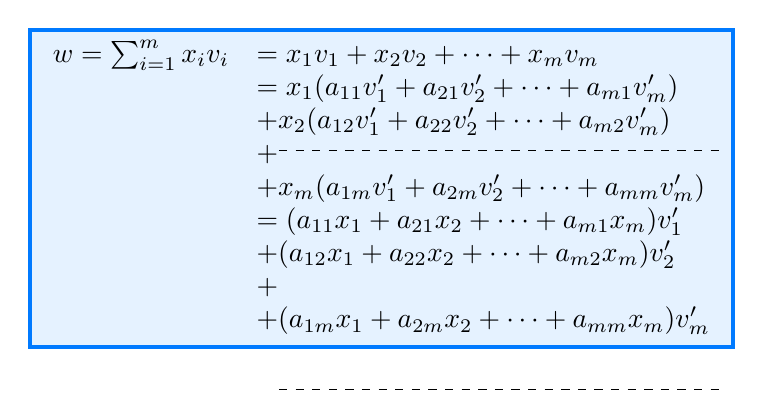
\begin{tikzpicture}
\node[draw=lightblue, rectangle, fill=lightblue!10, line width=1.5pt] {$\begin{array}{ll}
w=\sum_{i=1}^mx_iv_i & =x_1v_1+x_2v_2+\cdots+x_mv_m\\
 & =x_1(a_{11}v_1'+a_{21}v_2'+\cdots+a_{m1}v_m')\\
  & +x_2(a_{12}v_1'+a_{22}v_2'+\cdots+a_{m2}v_m')\\
  & + \\
  & +x_m(a_{1m}v_1'+a_{2m}v_2'+\cdots+a_{mm}v_m')\\
  & =(a_{11}x_1+a_{21}x_2+\cdots+a_{m1}x_m)v_1'\\
  & +(a_{12}x_1+a_{22}x_2+\cdots+a_{m2}x_m)v_2'\\
  & +\\
  & +(a_{1m}x_1+a_{2m}x_2+\cdots+a_{mm}x_m)v_m'\\
\end{array}$};
\draw[dashed] (-1.3,0.48) -- (4.3,0.48);
\draw[dashed] (-1.3,-2.55) -- (4.3,-2.55);
\end{tikzpicture}
\end{center}
Por tanto, \begin{center}
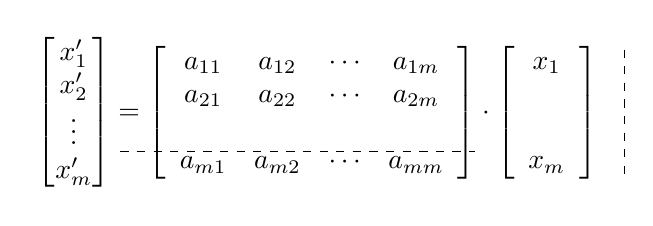
\begin{tikzpicture}
\node {$\begin{bmatrix}
x_1' \\ 
x_2' \\ 
\vdots \\
x_m'
\end{bmatrix}=\left[\begin{array}{cccc}
a_{11} & a_{12} & \cdots & a_{1m} \\ 
a_{21} & a_{22} & \cdots & a_{2m} \\ 
 &  &  &  \\ 
a_{m1} & a_{m2} & \cdots & a_{mm}
\end{array} \right]\cdot\left[\begin{array}{c}
x_{1} \\ 
 \\ 
 \\ 
x_{m}
\end{array} \right]$};
\draw[dashed] (-2.5,-0.5) -- (2,-0.5);
\draw[dashed] (3.9,0.8) -- (3.9,-0.8);
\end{tikzpicture}
\end{center} es decir, \begin{center}
\fbox{$[w]_{B'}=M_{B\rightarrow B'}[w]_{B}$}
\end{center}
\begin{wrapfigure}{r}{0.45\textwidth}
\begin{tikzpicture}
\node[draw=black, rectangle, line width=1.5pt] {
\begin{tikzpicture}
\draw[-latex, line width=1.5pt] (-2,0) -- (5,0);
\draw[-latex, line width=1.5pt] (0,-4) -- (0,3);
\draw[-latex, lightblue, line width=1.5pt] (0,0) -- (1,2);
\draw[-latex, lightblue, line width=1.5pt] (0,0) -- (2,-1);
\draw[-latex, blue, line width=1.5pt] (0,0) -- (1,-3);
\draw[-latex, blue, line width=1.5pt] (0,0) -- (0,-1);
\draw[lightblue, dashed] (0,2) -- (1,2) -- (1,0);
\draw[lightblue, dashed] (0,-1) -- (2,-1) -- (2,0);
\draw[blue, dashed] (0,-3) -- (1,-3) -- (1,0);
\end{tikzpicture}
};
\end{tikzpicture}
\end{wrapfigure}
\underline{Ejemplo}

$W=\mathbb{R}^2$

\textcolor{lightblue}{$B=\{v_1=(1,2),~v_2=(2,-1)\}$}

\textcolor{blue}{$B'=\{v_1'=(1,-3),~v_2'=(0,-1)\}$}

Vamos a calcular $M_{B\rightarrow B'}$.

$\begin{array}{rl}
v_{1}=(1,2) & =a_{11}v_1'+a_{21}v_2'\\
 & =a_{11}(1,-3)+a_{21}(0,-1)\\
 & =(a_{11},-3a_{11}-a_{21})
\end{array}$

\vspace{1cm}

$\left.\begin{array}{l}
1=a_{11}\\
2=-3a_{11}-a_{21}
\end{array}\right\rbrace\begin{array}{l}
\\
\longrightarrow a_{22}=-3a_{12}+1=-6+1=-5
\end{array}$

Por tanto, \[M_{B\rightarrow B'}=\begin{bmatrix}
1 & 2 \\ 
-5 & -5
\end{bmatrix} \]

Sea ahora $[v]_B=(1,1)$. ¿$[v]_{B'}$?

$[v_{B?}]=M_{B\rightarrow B'}[v]_B=\begin{bmatrix}
1 & 2 \\ 
-5 & -5
\end{bmatrix}\cdot\begin{bmatrix}
1\\
1
\end{bmatrix}=\begin{bmatrix}
3 & -10\\
\end{bmatrix}$

\textcolor{lightblue}{\underline{Coordenadas en bases ortonormales}}

Supongamos que $B=\{u_1,u_2,\hdots,u_m\}$ es una base ortonormal de W, es decir, \[u_i\cdot u_j=\delta_{\imath\jmath  }=\left\lbrace\begin{array}{l}
1 \text{ si }i=j\\
0 \text{ si }i\neq j
\end{array}\right.\text{delta de Kronecker}\]
$\|u_i\|,~1\le i\le m$

Vamos a calcular la forma que tiene $[w]_B$, siendo $w\in W$. Se tiene: \begin{center}
\fcolorbox{lightblue}{lightblue!10}{$w=\sum_{n=1}^{+\infty}x_1u_iu_j=x_j$}
\end{center}
Por tanto, \[[w]_B=(w\cdot u_j),~1\le j\le m\]
$\begin{array}{rl}
\text{Además, como }w\cdot u_j & =\|w\|\cdot\|u_j\|\cos(w,u_j)\\
 & =\|w\|\cdot\cos(w,u_j)
\end{array}$

Se tiene que si $\|w\|=1$, entonces \[\]

\begin{center}
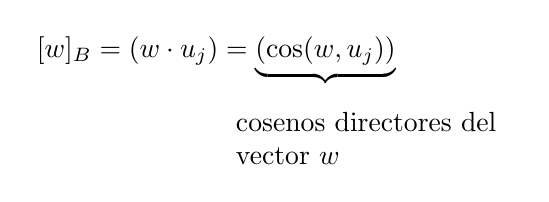
\begin{tikzpicture}
\node {$[w]_B=(w\cdot u_j)=\underbrace{(\cos(w,u_j))}$};
\node[text width=3.5cm] at (2,-1) {cosenos directores del vector $w$}; 
\end{tikzpicture}
\end{center}
Trabajar en bases ortonormales simplifica enormemente muchos de los cálculos que se hacen en Álgebra Lineal. Por ello, dada una base de un subespacio vectorial, interesa calcular, a partir de ella una nueva base ortonormal. El algoritmo de Gram-Schmidt nos permite conseguir este objetivo.

\textcolor{lightblue}{\underline{Método de ortogonalización de Gram-Schmidt y su versión matricial, factorización $A=QR$}}
\begin{itemize}[label=\color{red}\textbullet, leftmargin=*]
    \item \color{lightblue}Teorema (Factorización $QR$)
\end{itemize}
Sean $\{a_1,a_2,\hdots,a_n\}$ un conjunto de vectores de $\mathbb{R}^m$ linealmente independientes. Entonces, existe un conjunto ortonormal $\{q_1,q_2,\hdots,q_n\}$, entonces existe una matriz $R$ triangular superior con elementos positivos en la diagonal de modo que \[A=QR\]

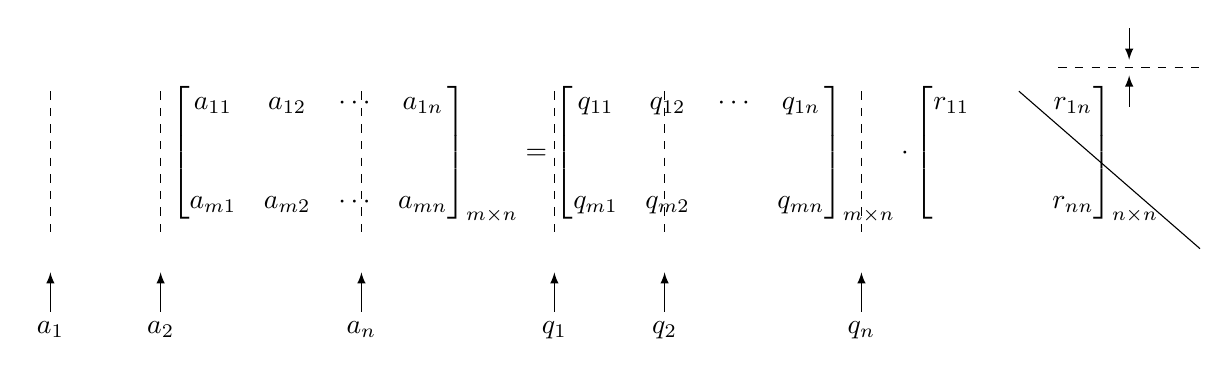
\begin{tikzpicture}[>=latex]
\node {$\begin{bmatrix}
a_{11} & a_{12} & \cdots & a_{1n} \\ 
 &  &  &  \\ 
 &  &  &  \\ 
a_{m1} & a_{m2} & \cdots & a_{mn}
\end{bmatrix}_{m\times n}=\begin{bmatrix}
q_{11} & q_{12} & \cdots & q_{1n} \\ 
 &  &  &  \\ 
 &  &  &  \\ 
q_{m1} & q_{m2} &  & q_{mn}
\end{bmatrix}_{m\times n}\cdot\begin{bmatrix}
r_{11} &  &  & r_{1n} \\ 
 &  &  &  \\ 
 &  &  &  \\ 
 &  &  & r_{nn}
\end{bmatrix}_{n\times n} $};
\draw[<-] (-7.8,-1.5) -- (-7.8, -2) node[below] {$a_1$};
\draw[<-] (-6.4,-1.5) -- (-6.4, -2) node[below] {$a_2$};
\draw[<-] (-3.85,-1.5) -- (-3.85, -2) node[below] {$a_n$};
\draw[<-] (-1.4,-1.5) -- (-1.4, -2) node[below] {$q_1$};
\draw[<-] (0,-1.5) -- (0, -2) node[below] {$q_2$};
\draw[<-] (2.5,-1.5) -- (2.5, -2) node[below] {$q_n$};
\draw (4.5,0.8) -- (6.8, -1.2);
\draw[dashed] (-7.8,0.8) -- (-7.8, -1);
\draw[dashed] (-6.4,0.8) -- (-6.4, -1);
\draw[dashed] (-3.85,0.8) -- (-3.85, -1);
\draw[dashed] (-1.4,0.8) -- (-1.4, -1);
\draw[dashed] (0,0.8) -- (0, -1);
\draw[dashed] (2.5,0.8) -- (2.5, -1);
\draw[dashed] (5,1.1) -- (6.8, 1.1);
\draw[->] (5.9, 1.6) -- (5.9,1.2) ;
\draw[<-] (5.9, 1) -- (5.9,0.6) ;
\end{tikzpicture}
\begin{itemize}[label=\color{red}\textbullet, leftmargin=*]
    \item \color{lightblue}Demostración
\end{itemize}
El algoritmo, el cual es constructivo, consta de las siguientes etapas o pasos:

\underline{Paso 1:} Tomamos $q=1=\dfrac{a_{1}}{\|a_1\|}$

Con lo que $a_1=\|a_1\|q_1$. Tenemos entonces $r_{11}=\|a_{11}\|$

\underline{Paso 2:} Tomamos $v_2=a_2+\alpha q_1$

Imponemos $q_1\cdot v_2=0$

$0=q_1\cdot v_2=q_1\cdot a_2+\alpha q_1\cdot q_1=q_1\cdot a_2+\alpha\longrightarrow \alpha=-q_1\cdot a_2$

Por tanto: $v_2=a_2-(q_1\cdot a_2)q_1$

$\begin{array}{rl}
\text{Calculamos }\|v_2\|^2 & =(a_2-(q_1\cdot a_2)q_1)\cdot(a_2-(q_1\cdot q_2)q_1)\\
 & =a_2\cdot a_2-(q_1\cdot a_2)^2-(q_1\cdot a_2)^2+(q_1\cdot a_2)^2\\
 & =a_2\cdot a_2-(q_1\cdot a_2)^2
\end{array}$

Con lo que $\|v_2\|=\left(\|a_2\|^2-(q_1\cdot a_2)^2\right)^{\frac{1}{2}}$

Tomamos entonces $q_2=\dfrac{v_2}{\|v_2\|}=\dfrac{1}{\left(\|a_2\|^2-(q_1\cdot a_2)^2\right)^{\frac{1}{2}}}\cdot\left(a_2-(q_1\cdot a_2)q_1\right)$

$r_{12}=-q_1\cdot a_2,~r_{22}=\left(\|a_2\|^2-(q_1\cdot a_2)^2\right)^{\frac{1}{2}}$ ya que $a_2=\underbrace{q_1\cdot a_2}_{r_{12}}q_1+\underbrace{\left(\|a_2\|^2-(q_1\cdot a_2)^2\right)^{\frac{1}{2}}}_{r_{22}}\cdot~q_{12}$

\underline{Paso 3:} Tomamos $v_3=a_3+\alpha q_1+\beta q_{12}$

Imponemos: 
\begin{enumerate}[label=\alph*)]
\item $0=v_3\cdot q_1=a_3\cdot q_1+\alpha\overbrace{q_1\cdot q_1}^{1}+\beta\overbrace{q_2\cdot q_1}^{0}\longrightarrow \alpha=-a_3q_1$
\item $0=v_3\cdot q_2=a_3\cdot q_2+\alpha\underbrace{q_1\cdot q_2}_{0}+\beta\underbrace{q_1\cdot q_1}_1\longrightarrow\beta=-a_3q_2$
\end{enumerate}
Finalmente, calculamos 

$$
\begin{array}{rcl}
\|v_3\|^2 & = &(a_3+\alpha q_1+\beta q_2)\cdot(a_3+\alpha q_1+\beta q_2)\\
 &=&\|a_3\|^2+\overline{\alpha q_1q_3}+\beta q_2\cdot a_3+\overline{\alpha q_1 q_3}+\alpha\overbrace{q_1\cdot q_1}^1+\\
 & &\alpha\beta q_1q_2+\beta q_2a_3+\alpha\beta q_1q_2+\beta\underbrace{q_2\cdot q_2}_1\\
 & =& \|a_3\|^2+2\alpha\beta q_1q_3+2\beta q_2a_3+\alpha+\beta
\end{array}
$$
Tomamos: $q_3=\dfrac{v_3}{\|v_3\|}=\dfrac{1}{\|v_3\|}\left(a_3-(a_3\cdot q_1)q_1-(a_3\cdot q_2)q_2\right)$

Con lo que: \[a_3=\underbrace{(a_3\cdot q_1)}_{r_{13}}q_1+\underbrace{(a_3\cdot q_2)}_{r_{23}}q_2+\underbrace{\|v_3\|}_{r_{33}}q_3\] y así sucesivamente.

\underline{Ejemplo}

\begin{center}
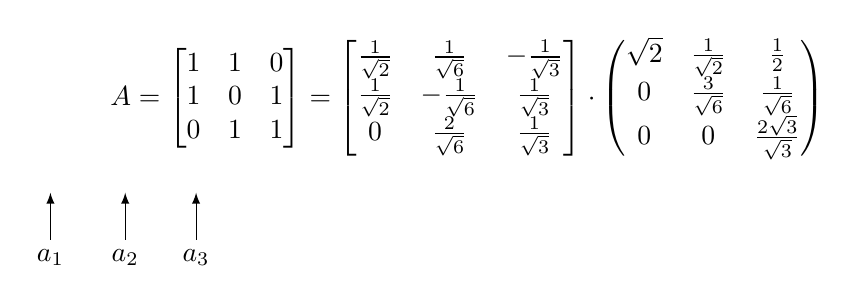
\begin{tikzpicture}[>=latex]
\node {$A=\begin{bmatrix}
1 & 1 & 0 \\ 
1 & 0 & 1 \\ 
0 & 1 & 1
\end{bmatrix}=\begin{bmatrix}
\frac{1}{\sqrt{2}} & \frac{1}{\sqrt{6}} & -\frac{1}{\sqrt{3}} \\ 
\frac{1}{\sqrt{2}} & -\frac{1}{\sqrt{6}} & \frac{1}{\sqrt{3}} \\ 
0 & \frac{2}{\sqrt{6}} & \frac{1}{\sqrt{3}}
\end{bmatrix}\cdot\begin{pmatrix}
\sqrt{2} & \frac{1}{\sqrt{2}} & \frac{1}{2} \\ 
0 & \frac{3}{\sqrt{6}} & \frac{1}{\sqrt{6}} \\ 
0 & 0 & \frac{2\sqrt{3}}{\sqrt{3}}
\end{pmatrix} $};
\draw[<-] (-5.3,-1.2) -- (-5.3,-1.8) node[below] {$a_1$};
\draw[<-] (-4.35,-1.2) -- (-4.35,-1.8) node[below] {$a_2$};
\draw[<-] (-3.45,-1.2) -- (-3.45,-1.8) node[below] {$a_3$};
\end{tikzpicture}
\end{center}
\begin{enumerate}[label=\arabic*)]
\item $q_1=\dfrac{a_1}{\|a_1\|},~\|a_1\|=\sqrt{1^2+1^2}=\sqrt{2}$

$q_1=\dfrac{1}{\sqrt{2}}a_1\longrightarrow a_1=\underbrace{\sqrt{2}}_{r_{11}}q_{11}$

\item $v_2=a_2+\alpha q_1$

$\begin{array}{rl}
0= & v_2\cdot q_1=a_2\cdot q_1+\alpha q_1\cdot q_1\longrightarrow\alpha=-a_2\cdot q_1=-(1,0,0)\cdot\dfrac{1}{\sqrt{2}}(1,1,0)\\
=& a_2-\dfrac{1}{\sqrt{2}}q_1=(1,0,1)-\left(\dfrac{1}{2},\dfrac{1}{2},0\right)=\left(\dfrac{1}{2},-\dfrac{1}{2},1\right)
\end{array}$

$\|v_2\|=\sqrt{\dfrac{1}{4}+\dfrac{1}{4}+1}=\sqrt{\dfrac{3}{2}}=\dfrac{3}{\sqrt{6}}$

$q_2=\dfrac{v_2}{\|v_2\|}=\dfrac{\sqrt{2}}{\sqrt{3}}\left(\dfrac{1}{2},\dfrac{1}{2},1\right)=\left(\dfrac{1}{\sqrt{6}},-\dfrac{1}{\sqrt{6}},\dfrac{2}{\sqrt{6}}\right)$

$a_2=\dfrac{1}{\sqrt{2}}q_1+v_2=\underbrace{\dfrac{1}{\sqrt{2}}}_{r_{12}}q_1+\underbrace{\|v_2\|}_{r_{22}}q_2$

\item $V_3=a_3+\alpha q_1+\beta q_2$

$0=q_1\cdot v_3\longrightarrow\alpha=a_3\cdot q_1=-(0,1,1)\cdot\left(\dfrac{1}{\sqrt{2}},\dfrac{1}{\sqrt{2}},0\right)=-\dfrac{1}{\sqrt{2}}$

$0=q_2\cdot v_3\longrightarrow\beta=-a_3\cdot q_2=-(0,1,1)\cdot\left(\dfrac{1}{\sqrt{6}},-\dfrac{1}{\sqrt{6}},\dfrac{2}{\sqrt{6}}\right)=\dfrac{1}{\sqrt{6}}-\dfrac{2}{\sqrt{6}}=-\dfrac{1}{\sqrt{6}}$

$v_3=(0,1,1)-\dfrac{1}{\sqrt{2}}\left(\dfrac{1}{\sqrt{2}},\dfrac{1}{\sqrt{2}},0\right)-\dfrac{1}{\sqrt{6}}\left(\dfrac{1}{\sqrt{6}},-\dfrac{1}{\sqrt{6}},\dfrac{2}{\sqrt{6}}\right)=$

$(0,1,1)-\left(\dfrac{1}{2},\dfrac{1}{2},0\right)-\left(\dfrac{1}{6},-\dfrac{1}{6},\dfrac{2}{6}\right)=\left(-\dfrac{2}{3},\dfrac{2}{3},\dfrac{2}{3}\right)$

$\|v_3\|=\sqrt{\dfrac{4}{9}+\dfrac{4}{9}+\dfrac{4}{9}}\sqrt{\dfrac{12}{9}}=\dfrac{2}{3}\sqrt{3}$

$q_3=\dfrac{v_3}{\|v_3\|}=\dfrac{2\sqrt{3}}{3}\left(-\dfrac{2}{3},\dfrac{2}{3},\dfrac{2}{3}\right)=\left(-\dfrac{1}{\sqrt{3}},\dfrac{1}{\sqrt{3}},\dfrac{1}{\sqrt{3}}\right)$

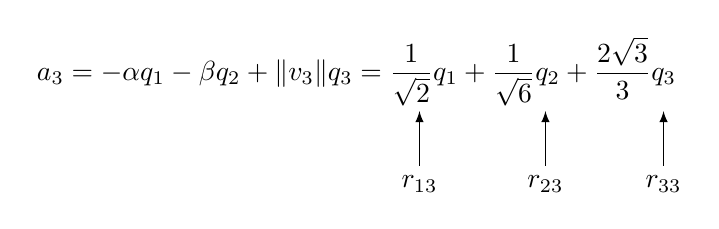
\begin{tikzpicture}[>=latex]
\node {$a_3=-\alpha q_1-\beta q_2+\|v_3\|q_3=\dfrac{1}{\sqrt{2}}q_1+\dfrac{1}{\sqrt{6}}q_2+\dfrac{2\sqrt{3}}{3}q_3$};
\draw[<-] (0.8,-0.5) -- (0.8,-1.2) node[below] {$r_{13}$};
\draw[<-] (2.4,-0.5) -- (2.4,-1.2) node[below] {$r_{23}$};
\draw[<-] (3.9,-0.5) -- (3.9,-1.2) node[below] {$r_{33}$};
\end{tikzpicture}
\end{enumerate}
\begin{itemize}
\item[\underline{Nota:}] Si $A$ es una matriz cuadrada, entonces la condición $\det(A)\neq0$ garantiza que las columnas de $A$ son linealmente independientes y por tanto, la existencia de la factorización $A=QR$ está garantizado.
\end{itemize}
\textcolor{lightblue}{\underline{Proyección ortogonal}}

Sean $W\subset\mathbb{R}^n$ un subespacio y $x\in\mathbb{R}^n$.

\begin{center}
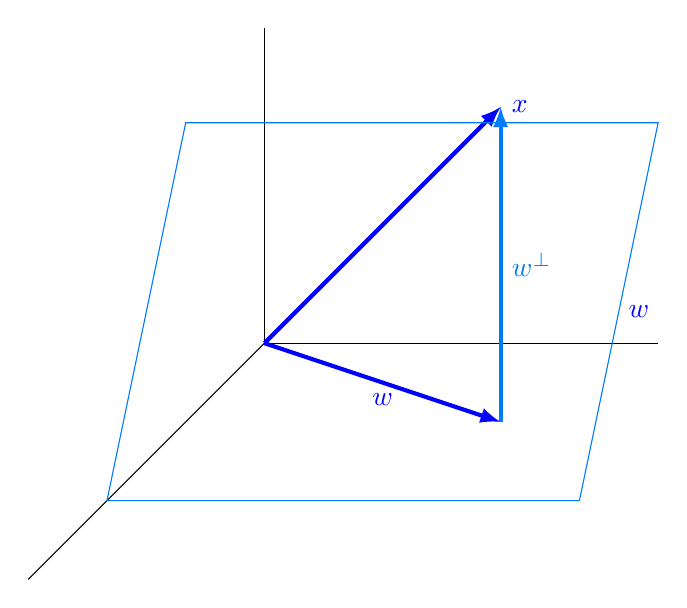
\begin{tikzpicture}[>=latex]
\draw (0,0) -- (5,0);
\draw (0,0) -- (0,4);
\draw (0,0) -- (-3,-3);
\draw[->, blue, line width=1.5pt] (0,0) -- (3,3) node[right] {$x$};
\draw[->, blue, line width=1.5pt] (0,0) -- (3,-1) node[midway,below] {$w$}; 
\draw[->, lightblue, line width=1.5pt] (3,-1) -- (3,3) node[midway, right] {$w^\bot$};
\draw[lightblue] (-2,-2) -- (-1, 2.8) -- (5,2.8)  -- (4,-2)node[midway, right, blue] {$w$} -- cycle;
\end{tikzpicture}
\end{center}
¿Cuál es el vector de $W$ que está más cerca de $x$?

Es decir, $\min_{w\in W}\|w-x\|$

Dado $x\in \mathbb{R}^n$, se puede ver que $x=w+w^\bot$ con $w\in W$ y $w^\bot\in W^\bot$, subespacio al que llamaremos ortogonal de $W$. En concreto: \begin{center}
\fcolorbox{lightblue}{lightblue!10}{$w^\bot:\left\lbrace\overline{W}\in\mathbb{R}^n:\overline{w}\cdot w=0~~\forall w\in W\right\rbrace$}
\end{center}
Es decir, $\mathbb{R}^n=W\oplus W^\bot$, donde $\oplus$ significa:
\begin{enumerate}[label=\roman*)]
\item $\mathbb{R}^n=W+W^\bot$
\item $W\cap W^\bot=\{0\}$
\end{enumerate}
y se habla de \textcolor{lightblue}{suma discreta}.

Al vector $w$ en la descomposición $x=w+w^\bot$ se le llama \textcolor{lightblue}{proyección ortogonal de $x$ en $W$}.

Escribimos $w=\mathbb{P}_w(x)$.

Veamos cómo se calcula. Sea $\{u_1,\hdots,u_m\}$ una base ortonormal de $W$, y $\{u_{m+1},\hdots,u_n\}$ una base ortonormal de $W^\bot$. Resulta entonces que \[\{u_{1},u_{2},\hdots,u_m,u_{m+1},\hdots,u_n\}\] es una base ortonormal de $\mathbb{R}^n$. Por tanto \begin{center}
\fcolorbox{lightblue}{lightblue!10}{$x=w+w^\bot=\sum_{i=1}^nx_iu_i=\sum_{i=1}^mx_iu_i+\sum_{i=m+1}^mx_iu_i$}
\end{center}
Se tiene entonces que \[x\cdot u_j=x_j\]
Por tanto, $w=\sum_{i=1}^mx_iu_i$ tiene coordenadas \begin{center}
\fbox{$x_i=x\cdot u_i$}
\end{center}
\underline{Ejemplo}

Calcula la proyección ortogonal en $\mathbb{R}^3$ del vector $v=(0,-1,0)$ sobre el plano de ecuación $x+y+z=0$.

\begin{center}
\begin{tikzpicture}[>=latex]
\draw[<->] (-3,0) -- (5,0);
\draw[->] (0,0) -- (0,4);
\draw[->] (0,0) -- (-3,-3);
\draw[lightblue] (2,3) -- (-2.5,-1) -- (-3,-2) -- (1.5,-2) -- (3,3);
\node[lightblue] at (2.5, 3) {\Large $\mathbb{R}^3$};
\node[text width=6cm] at (7,2) {$\vec{n}=(1,1,1)$ vector normal al plano};
\end{tikzpicture}
\end{center}
$W=\left\lbrace(x,y,z)\in\mathbb{R}^3:x+y+z=0\right\rbrace$

Tomamos dos parámetros

$\begin{array}{l}
z=\alpha\\
y=\beta\\
x=-z-y=-\alpha-\beta
\end{array}$\hspace{2cm}\begin{tikzpicture}[baseline=(current bounding box.center)]
\node {$\begin{bmatrix}
x \\ 
y \\ 
z
\end{bmatrix}=\alpha\cdot\begin{bmatrix}
-1\\
0\\
1
\end{bmatrix}+\beta\cdot\begin{bmatrix}
-1\\
1\\
0
\end{bmatrix} $};
\draw[latex-] (-0.1,-1.2) -- (-0.1,-2) node[below] {$v_1$};
\draw[latex-] (2.05,-1.2) -- (2.05,-2) node[below] {$v_2$};
\end{tikzpicture}

$\|v_1\|=\sqrt{2};~\|v_2\|=\sqrt{2}$

Construimos una base ortonormal de $W$ usando el algoritmo de Gram-Schmidt.

$u_1=\dfrac{v_1}{\|v_1\|}=\dfrac{1}{\sqrt{2}}(-1,1,0)$

$v_2=(-1,0,1)+\alpha\dfrac{1}{\sqrt{2}}(-1,1,0)$

$0=v_2\cdot u_1=(-1,0,1)\cdot\dfrac{1}{\sqrt{2}}(-1,1,0)+\alpha$

$\alpha=-\dfrac{1}{\sqrt{2}}(-1,0,1)\cdot(-1,1,0)=-\dfrac{1}{\sqrt{2}}$

$v_2=(-1,0,1)-\dfrac{1}{\sqrt{2}}\cdot\dfrac{1}{\sqrt{2}}(-1,1,0)=(-1,0,1)+\left(\dfrac{1}{2},-\dfrac{1}{2},0\right)=\left(-\dfrac{1}{2},-\dfrac{1}{2},1\right)$

$\|v_2\|=\sqrt{\dfrac{1}{4}+\dfrac{1}{4}+1}=\sqrt{\dfrac{3}{2}}$

Finalmente, $u_2=\dfrac{\sqrt{3}}{\sqrt{2}}\left(-\dfrac{1}{2},-\dfrac{1}{2},1\right)$

$\mathbb{P}_w(u)=(v\cdot u_1)u_1+(v\cdot u_2)u_2$

\textcolor{lightblue}{\underline{Transformaciones (Aplicaciones) lineales}}
\begin{itemize}[label=\color{red}\textbullet, leftmargin=*]
    \item \color{lightblue} Definición
\end{itemize}
Una transformación o aplicación lineal es una aplicación \[f:\mathbb{K}^n\longrightarrow\mathbb{K}^n\] que cumple las dos siguientes propiedades: 
\begin{enumerate}[label=\arabic*)]
\item $f(u+v)=f(u)+f(v)~~\forall u,v\in\mathbb{K}^n$
\item $f(\alpha u)=\alpha f(u)$
\end{enumerate}
\underline{Ejemplo}

$f:\mathbb{R}^2\longrightarrow\mathbb{R}^2$

$(x,y)\longmapsto f(x,y)=(x\cos\theta-y\sin\theta, x\sin\theta+y\cos\theta)$

$\theta$ es un ángulo fijo.

Veamos que $f$ cumple las dos propiedades anteriores:
\begin{enumerate}[label=\arabic*)]
\item $u=(x_1,y_1),v=(x_2,y_2)$

$u+v=(x_1+x_2,y_1+y_2)$

$f(u+v)=f(x_1+x_2,~y_1+y_2)=\left((x_1+x_2)\cos\theta-(y_1+y_2)\sin\theta,~(x_1+x_2)\sin\theta-(y_1+y_2)\cos\theta\right)=(x_1\cos\theta-y_1\sin\theta,~x_1\sin\theta+y_1\cos\theta)+(x_2\cos\theta-y_2\sin\theta,~x_2\sin\theta+y_2\cos\theta)=f(u)+f(v)$
\item $f(\alpha u)=f\left(\alpha(x_1,~y_1)\right)=f(\alpha x_1,~\alpha y_1)=(\alpha x_1\cos\theta-\alpha y_1\sin\theta,~\alpha x_1\sin\theta+\alpha y_1\cos\theta)=\alpha(x_1\cos\theta-y_1\sin\theta,~x_1\sin\theta+y_1\cos\theta)=\alpha f(u)$
\end{enumerate}
\begin{itemize}[label=\color{red}\textbullet, leftmargin=*]
    \item \color{lightblue} Significado geométrico de $f$
\end{itemize}
$f(1,0)=(\cos\theta,~\sin\theta)$

$f(0,1)=(-\sin\theta,~\cos\theta)$

\begin{center}
\begin{tikzpicture}[scale=2, baseline=(current bounding box.center), >=latex]
\draw (-1,0) -- (2,0);
\draw (0,-1) -- (0,2);
\draw[->, lightblue, line width=1.5pt] (0,0) -- (1,0) node[below] {$(1,0)$};
\draw[->, lightblue, line width=1.5pt] (0,0) -- (0,1) node[right] {$(0,1)$};
\end{tikzpicture}
\hspace{1cm}
\begin{tikzpicture}[scale=2, baseline=(current bounding box.center), >=latex]
\draw (-2,0) -- (2,0);
\draw (0,-1) -- (0,2);
\draw[->, lightblue, line width=1.5pt] (0,0) -- (-1,1) node[left] {$f(0,1)$};
\draw[->, lightblue, line width=1.5pt] (0,0) -- (1.2,1.2) node[right] {$f(1,0)$};
\draw[dashed, lightblue, line width=1.5pt] (0,1) -- (-1,1) -- (-1,0);
\draw[dashed, lightblue, line width=1.5pt] (0,1.2) -- (1.2,1.2) -- (1.2,0);
\draw[blue, line width=1.5pt] (-0.5,0.5) to[bend left] (0.5,0.5) ;
\draw[blue, line width=1.2pt, ->] (0.4,0) arc (0:45:0.4) node[midway, right] {$\theta$};
\end{tikzpicture}
\end{center}
$f$ es un giro de $\theta$ grados. 

Además, por linealidad:

\begin{align*}
f(x,y)&=f\left(x(1,0)+y(0,1)\right)\\
&=xf(1,0)+yf(0,1)\\
&=x(\cos\theta,~\sin\theta)+y(-\sin\theta,~\cos\theta)\\
&=\begin{bmatrix}
\cos\theta & -\sin\theta \\ 
\sin\theta & \cos\theta
\end{bmatrix}\cdot\begin{bmatrix}
x\\
y
\end{bmatrix} =\begin{bmatrix}
\cos\theta\\
\sin\theta
\end{bmatrix}x+\begin{bmatrix}
-\sin\theta\\
\cos\theta
\end{bmatrix}y
\end{align*}
Lo anterior nos sugiere que dada una aplicación lineal $f:\mathbb{K}^n\longrightarrow\mathbb{K}^n$ y fijados bases $B$ de $\mathbb{K}^n$ y $B'$ de $\mathbb{K}^m$ existe $f$ se dice una aplicación lineal ortogonal porque su matriz es ortogonal.
\begin{itemize}[label=\color{red}\textbullet, leftmargin=*]
    \item \color{lightblue}Matriz asociada a una aplicación lineal
\end{itemize}
Sean $B=\{v_1,v_,\hdots,v_n\}$ y $B'=\{v_1',v_2',\hdots,v_n'\}$ bases de $\mathbb{K}^n$ y $\mathbb{K}^m$, respectivamente.

Dada $f:\mathbb{K}^n\longrightarrow\mathbb{K}^m$, se tiene 
\begin{center}
\begin{tikzpicture}
\node {$\begin{array}{l}
f(v_1)=a_{11}v_1'+a_{21}v_2'+\cdots+a_{m1}v_m'\\
f(v_2)=a_{12}v_1'+a_{22}v_2'+\cdots+a_{m2}v_m'\\
\\
f(v_n)=a_{1n}v_1'+a_{2n}v_2'+\cdots+a_{mn}v_m'
\end{array}$};
\draw[dashed] (-3.2,-0.5) -- (3.1,-0.5);
\end{tikzpicture}
\end{center}
A la matriz \[M_{B\rightarrow B'}(f)=\begin{bmatrix}
a_{11} & a_{12} & \cdots & a_{1n} \\ 
a_{21} & a_{22} & \cdots & a_{2n} \\ 
\vdots & \vdots &  & \vdots \\ 
a_{m1} & a_{m2} &  & a_{mn}
\end{bmatrix} \]
se le llama matriz asociada a $f$ en las bases $B$ y $B'$.

Obviamente, se tiene que dado $x=x_1v_1+\cdots+x_nv_n$, entonces \begin{center}
\fcolorbox{lightblue}{lightblue!10}{$f(x)=M_{B\rightarrow B'}(f)\cdot x_B$}
\end{center} con \[x_B=\begin{bmatrix}
x_1\\
\vdots\\
x_n
\end{bmatrix}\]
\begin{itemize}[label=\color{red}\textbullet, leftmargin=*]
    \item \color{lightblue} Cambio de coordenadas (o de base)
\end{itemize}
Sea $f:\mathbb{R}^n\longrightarrow\mathbb{R}^n$. Consideremos la base canónica de $\mathbb{R}^n$, denotada por $\mathcal{C}$, y $B$ es una base distinta de $\mathbb{R}^n$. Entonces, obviamente
\[M_{C\rightarrow\mathcal{C}}(f)\neq M_{BB}(f)\]
\[\begin{array}{rcl}
f: \mathbb{R}^n & \xrightarrow{\hspace{1.5cm}} & \mathbb{R}^n\\
B & & B\\
\mathcal{C} & & \mathcal{C}
\end{array}\]
¿Qué relación existe entre las matrices anteriores?
\begin{center}
\begin{tikzpicture}[baseline=(current bounding box.center), scale=1.5, >=latex]
\node (A) at (0,0) {$\mathbb{R}^n$};
\node (B) at (0,2) {$\mathbb{R}^n$};
\node (C) at (2,2) {$\mathbb{R}^n$};
\node (D) at (2,0) {$\mathbb{R}^n$};
\draw[->] (A) -- (B);
\draw[->] (B) -- (C) node[midway, below] {$f$};
\draw[->] (C) -- (D);
\draw[->] (A) -- (D) node[midway, below] {$f$};
\node at (-0.3, 1.7) {$\mathcal{C}$};
\node at (2.3, 1.7) {$\mathcal{C}$};
\node at (-0.3, -0.3) {$B$};
\node at (2.3, -0.3) {$B$};
\end{tikzpicture}
\hspace{2cm}
$\begin{array}{l}
M_{\mathcal{C}\rightarrow\mathcal{C}}(f)\\
\\
M_{B\rightarrow B}(f)
\end{array}$
\end{center}
\begin{itemize}[label=\color{red}\textbullet, leftmargin=*]
    \item \color{lightblue} Proposición
\end{itemize}
Se cumple \begin{center}
\fcolorbox{lightblue}{lightblue!10}{$M_{B\rightarrow B}(f)=M_{C\rightarrow B}\cdot M_{C\rightarrow C}(f)\cdot M_{B\rightarrow C}$}
\end{center} 
$\begin{array}{ll}
\text{donde }& M_{B\rightarrow\mathcal{C}} \text{ es la misma matriz de cambio de base de }B \text{ a } \mathcal{C}\\
& M_{\mathcal{C}\rightarrow B}=(M_{B\rightarrow\mathcal{C}})^{-1} \text{ es la misma matriz de cambio de base de }\mathcal{C} \text{ a } B\\
\end{array}$
\begin{itemize}[label=\color{red}\textbullet, leftmargin=*]
    \item \color{lightblue}Demostración
\end{itemize}
Recordemos \[x_B=M_{C\rightarrow B}X_{\mathcal{C}}\] y por tanto \[X_{\mathcal{C}}=(M_{C\rightarrow B)}^{-1}\cdot x_B=M_{B\rightarrow C}\cdot x_B\]
Por tanto: 
\begin{center}
\begin{tikzpicture}
\node[draw=lightblue, fill=lightblue!10, line width=1.5pt, text width=12cm, rectangle] {$\left(f(x_B)\right)_B=M_{C\rightarrow B}f(x_B)_{\mathcal{C}}=M_{C\rightarrow B}\cdot M_{\mathcal{C}\mathcal{C}}(f)(x_B)_{\mathcal{C}}=$\\$M_{C\rightarrow B}\cdot M_{C\rightarrow C}(f)\cdot(M_{C\rightarrow B)}^{-1}\cdot x_B=M_{C\rightarrow B}\cdot M_{C\rightarrow\mathcal{C}}(f)\cdot M_{B\rightarrow\mathcal{C}}~x_B$
};
\end{tikzpicture}
\end{center}
\underline{Importante:} Si dos matrices $M$ y $N$ están relacionadas en la forma $N=P^{-1}MP$, con $P$ invertible, entonces ambas matrices están asociadas a la misma aplicación lineal pero en dos bases distintas.

\textcolor{lightblue}{\underline{Valores y vectores propios}}

\begin{itemize}[label=\color{red}\textbullet, leftmargin=*]
    \item \color{lightblue} Definición
\end{itemize}
Sea $A\in M_n(\mathbb{K}^n)$. Se dice que $\lambda$ es un valor propio o autovalor (eigenvalue) de $A$ si existe un vector no nulo $v\in \mathbb{K}^n$, llamando vector propio o autovector (eigenvector) de modo que $Au=\lambda v$.

Al conjunto de todos los valores propios de $A$ se le llama espectro de $A$. Al mayor, en valor absoluto, de los autovalores se le llama radio espectral, denotado $\mathrm{p}(A)$, o valor propio dominante.
\begin{itemize}
\item[$\longrightarrow$] ¿Cómo calculamos los autovalores y autovectores de una matriz? 
\end{itemize}
$Au=\lambda v\longleftrightarrow(A-\lambda I)v=0\longleftrightarrow v\in\mathrm{Nuc}(A-\lambda I)\neq\{0\}\longleftrightarrow\mathrm{dimNuc}(A-\lambda I)=n-\mathrm{r}(A-\lambda I)\ge1\longleftrightarrow\mathrm{r}(A-\lambda I)< n\longleftrightarrow\mathrm{det}(A-\lambda I)=0$
\begin{itemize}[label=\color{red}\textbullet, leftmargin=*]
    \item \color{lightblue} Definición (Polinomio característico)
\end{itemize}
Sea $A\in M_n(\mathbb{K}^n)$. Se llama polinomio característico de $A$, denotado $P_A(\lambda)$, al polinomio \begin{center}
\fcolorbox{lightblue}{lightblue!10}{$P_A(\lambda)=\det(A-\lambda I)$}
\end{center}
Valores propios $\lambda_1=9,~\lambda_2=1$
\begin{itemize}[label=\color{red}\textbullet, leftmargin=*]
    \item \color{lightblue} Vectores propios
\end{itemize}
$\lambda_1=9$\hspace{1cm}$K_{er}(A-9I)=K_{er}\begin{pmatrix}
-4 & 4 \\ 
4 & -4
\end{pmatrix} $

$\begin{bmatrix}
-4 & 4 \\ 
4 & -4
\end{bmatrix}\cdot\begin{bmatrix}
x\\
y
\end{bmatrix}=\begin{bmatrix}
0\\
0
\end{bmatrix} $

$\left.\begin{array}{r}
-4x+4y=0\\
4x-4y=0
\end{array}\right\rbrace\begin{array}{l}
y=\alpha\longrightarrow x=\alpha\\
K_{er}(A-9I)=<(1,1)>
\end{array}$

$\lambda_2=1$\hspace{1cm}$K_{er}(A-9I)=K_{er}\begin{pmatrix}
4 & 4 \\ 
4 & 4
\end{pmatrix} $

$\begin{bmatrix}
4 & 4 \\ 
4 & 4
\end{bmatrix}\cdot\begin{bmatrix}
x\\
y
\end{bmatrix}=\begin{bmatrix}
0\\
0
\end{bmatrix} $

$\left.\begin{array}{r}
4x+4y=0\\
4x+4y=0
\end{array}\right\rbrace\begin{array}{l}
y=\alpha\longrightarrow x=-\alpha\\
K_{er}(A-I)=<(-1,1)>
\end{array}$

Consideremos la matriz $P$ formada por los valores propios anteriores pero unitarios, es decir \[P=\begin{bmatrix}
\dfrac{1}{\sqrt{2}} & -\dfrac{1}{\sqrt{2}} \\ 
\dfrac{1}{\sqrt{2}} & \dfrac{1}{\sqrt{2}}
\end{bmatrix} \]
Nótese que $P$ es ortogonal. Por tanto $P^{-1}=P^T$.

Interpretación en términos de aplicaciones lineales

\begin{itemize}
\item[] $f:\mathbb{R}^2\longrightarrow\mathbb{R}^2$

$(x,y)\longmapsto f(x,y)=(5x+4y,~4x+5y)$

$C=\{(1,0),~(0,1)\}$

$A=M_{C\rightarrow C}(f)=\begin{bmatrix}
5 & 4 \\ 
4 & 5
\end{bmatrix} $

$f(1,0)=(5,4)=5\cdot(1,0)+4\cdot (0,1)$

$f(0,1)=(4,5)=4\cdot(1,0)+5\cdot(0,1)$

$B=\left\lbrace\left(\dfrac{1}{\sqrt{2}},\dfrac{1}{\sqrt{2}}\right),\left(-\dfrac{1}{\sqrt{2}},\dfrac{1}{\sqrt{2}}\right)\right\rbrace$

$f\left(\dfrac{1}{\sqrt{2}},\dfrac{1}{\sqrt{2}}\right)=\left(5\cdot\dfrac{1}{\sqrt{2}}+4\cdot\dfrac{1}{\sqrt{2}},~4\cdot\dfrac{1}{\sqrt{2}}+5\cdot\dfrac{1}{\sqrt{2}}\right)=9\left(\dfrac{1}{\sqrt{2}},\dfrac{1}{\sqrt{2}}\right)$

$f\left(-\dfrac{1}{\sqrt{2}},\dfrac{1}{\sqrt{2}}\right)=\left(-5\cdot\dfrac{1}{\sqrt{2}}+4\cdot\dfrac{1}{\sqrt{2}},~4\cdot-\dfrac{1}{\sqrt{2}}+5\cdot\dfrac{1}{\sqrt{2}}\right)=\left(-\dfrac{1}{\sqrt{2}},\dfrac{1}{\sqrt{2}}\right)$

$A=M_{B\rightarrow B}(f)=\begin{bmatrix}
9 & 0 \\ 
0 & 1
\end{bmatrix} $
\end{itemize}
\begin{itemize}[label=\color{red}\textbullet, leftmargin=*]
    \item \color{lightblue} Definición (Factorización en valores propios)
\end{itemize}
Sea $A\in M(\mathbb{K}^n)$. Se dice que $A$ es diagonalizable si existe una matriz diagonal $D$, con los valores propios de $A$ en su diagonal , y una matriz invertible $P$ cuyas columnas están formadas por vectores propios de $A$, de modo que \begin{center}
\fbox{$A=PDP^{-1}$}
\end{center}
A esta factorización se le llama factorización en valores propios.

\textcolor{lightblue}{\underline{Matrices simétricas}}

\begin{itemize}[label=\color{red}\textbullet, leftmargin=*]
    \item \color{lightblue}Teorema
\end{itemize}
Si $A\in M_n(\mathbb{R})$ es simétrica, entonces \[A=PDP^{-1}\] con $D=\mathrm{diag}(\lambda_1,\hdots,\lambda_n),~\lambda_j$ valores propios y $P=[u_1,\hdots,u_n]$ base ortonormal de vectores propios. 
\begin{itemize}[label=\color{red}\textbullet, leftmargin=*]
    \item \color{lightblue} Método $QR$
\end{itemize} 
\begin{itemize}[label=$\longrightarrow$]
\item Se utiliza para calcular todos los valores y vectores propios. 
\item Es muy estable porque al ser $Q$ ortogonal, no se propagan errores en los datos.
\end{itemize}
\begin{itemize}[label=\color{red}\textbullet, leftmargin=*]
    \item \color{lightblue} Algoritmo
\end{itemize}

1) Inicialización: tomar $A_0=A$

2) Iteración: para $k\ge0~~d_0$:

\hspace{1cm} 2.1) $A_0=Q_1R_1$ factorización $QR$ de $A_0$

\hspace{1cm} 2.2) $A_1=R_1Q_1$

\hspace{1cm}\underline{Nota:} $A_1=Q_1^TQ_1R_1Q_1=Q_1^TA_0Q_1$

\hspace{1cm}2.3) Factorización $QR$ de $A_1$

\hspace{1.5cm} $A_1=Q_2R_2$

\hspace{1cm} $A_2=R_2Q_2$

\hspace{1cm}\underline{Nota:} $A_2=Q_2^TQ_2R_2Q_2=Q_2^TA_1Q_2=Q_2^TQ_1^TA_0Q_1Q_2$ y así sucesivamente

\textcolor{lightblue}{\underline{Factorización en valores singulares (SVD)}}

El principal inconveniente de la factorización en valores propios es que sólo se puede aplicar a matrices cuadradas. De hecho, además las matrices han de ser simétricas para garantizar dicha factorización. Sin embargo, en Ciencia de Datos, aparecen muchas matrices que no son cuadradas ni tampoco simétricas. La factorización $SVD$ soluciona ambos problemas y para muchos \textcolor{lightblue}{es el resultado más importante de la Ciencia de Datos}.

\begin{itemize}[label=\color{red}\textbullet, leftmargin=*]
    \item \color{lightblue} Definición
\end{itemize}
Dada $A\in M_{m\times n}(\mathbb{R})$, se llama factorización $SVD$ (Singular Value Descomposition) de $A$ a una factorización de la forma \begin{center}
\fcolorbox{lightblue}{lightblue!10}{$A=U\Sigma V^T$}
\end{center} donde $\Sigma$ es una matriz diagonal con $\sigma_1,\hdots,\sigma_n$ en su diagonal $\Sigma\in M_{m\times n}(\mathbb{R})$.
\begin{itemize}[label=\color{red}\textbullet, leftmargin=*]
    \item \color{lightblue}Demostración
\end{itemize}
\begin{center}
\begin{tikzpicture}
	% Cuadrado A
	\node[style={minimum size=2cm,draw}] (A) at (0,0) {$A$};
	
	% Cuadrado U
	\node[style={minimum size=2cm,draw}] (U) at (3,0) {$U$};
	
	% Cuadrado matriz sigma
	\node[style={minimum size=2cm,draw}] (Sigma) at (6,0) {$\begin{matrix}
			\sigma_1 &  &  \\ 
			& \ddots &  \\ 
			&  & \sigma_n
		\end{matrix}$};
	
	% Cuadrado V^T
	\node[style={minimum size=2cm,draw}] (VT) at (9,0) {$V^T$};
	
   \node at (1.5,0) {$=$};
   \node at (4.25,0) {$\cdot$};
   \node at (7.75,0) {$\cdot$};
\end{tikzpicture}
\end{center}
\begin{itemize}[label=$\longrightarrow$]
\item Para que podamos colocar todos los valores singulares $m\ge n$, es decir, el número de filas de $\Sigma$ tiene que ser mayor o igual que el de columnas.
\end{itemize}
Sea $m\le n$, aplicamos el resultado a $A^T$ con lo que \begin{center}
\fcolorbox{lightblue}{lightblue!10}{$A^T=U\Sigma V^T$}\end{center} de donde tomamos traspuestas \begin{center}
\fcolorbox{lightblue}{lightblue!10}{$A^T=V\Sigma^TU^T$}
\end{center}
Definimos $U=[u_1,\hdots,u_m]$.

Se tiene \[U^TA\cdot V=\begin{bmatrix}
u_1^T\\
\vdots\\
u_m^T
\end{bmatrix}\cdot A[v_1,\hdots,v_n]=\begin{bmatrix}
u_1^T\\
\vdots\\
u_m^T
\end{bmatrix}\cdot[Av_1,\hdots,Av_n]= \]
\[\begin{bmatrix}
u_1^T\\
\vdots\\
u_m^T
\end{bmatrix}\cdot[\sigma_1 u_1,\hdots,\sigma_ru_r,0,\hdots,0]=[\sigma_1e_1,\hdots,\sigma_re_r,0,\hdots,0]=\Sigma\]
Multiplicando a la derecha por $V^{-1}=V^T$ y a la izquierda por $U$ se tiene \begin{center}
\fcolorbox{lightblue}{lightblue!10}{$A=U\Sigma V^T$}
\end{center}
\begin{itemize}[label=\color{red}\textbullet, leftmargin=*]
    \item \color{lightblue}Vectores propios
\end{itemize}
$\lambda_1=8~~K_{er}(A^TA-8I)$

$\begin{bmatrix}
-3 & 3 \\ 
3 & -3
\end{bmatrix}\cdot\begin{bmatrix}
x\\
y
\end{bmatrix}=\begin{bmatrix}
0\\
0
\end{bmatrix}\hspace{1cm}\left.\begin{array}{r}
-3x+3y=0\\
3x-3y=0
\end{array}\right\rbrace\longrightarrow x=y\longrightarrow v_1=\dfrac{1}{\sqrt{2}}(1,1)$

$\lambda_2=2~~K_{er}(A^TA-2I)$

$\begin{bmatrix}
3 & 3 \\ 
3 & 3
\end{bmatrix}\cdot\begin{bmatrix}
x\\
y
\end{bmatrix}=\begin{bmatrix}
0\\
0
\end{bmatrix}\hspace{1cm}\left.\begin{array}{r}
3x+3y=0\\
3x+3y=0
\end{array}\right\rbrace\longrightarrow x=-y\longrightarrow v_1=\dfrac{1}{\sqrt{2}}(-1,1)$

Matriz $V=\begin{bmatrix}
\dfrac{1}{\sqrt{2}} & -\dfrac{1}{\sqrt{2}} \\ 
\dfrac{1}{\sqrt{2}} & \dfrac{1}{\sqrt{2}}
\end{bmatrix} $

Valores singulares: $\sigma=\sqrt{8},~\sigma_2=\sqrt{2}\longrightarrow\Sigma=\begin{bmatrix}
\sqrt{8} & 0 \\ 
0 & \sqrt{2}
\end{bmatrix} $
\begin{itemize}[label=\color{red}\textbullet, leftmargin=*]
    \item \color{lightblue}Cálculo de la matriz $U$
\end{itemize}
$u_1=\dfrac{1}{\sigma_1}Av_1=\dfrac{1}{\sqrt{8}}\begin{bmatrix}
2 & 2 \\ 
-1 & 1
\end{bmatrix}\cdot\begin{bmatrix}
\dfrac{1}{\sqrt{2}}\\
\dfrac{1}{\sqrt{2}}
\end{bmatrix}=\begin{bmatrix}
1\\
0
\end{bmatrix} $

$u_2=\dfrac{1}{\sigma_2}Av_2=\dfrac{1}{\sqrt{2}}\begin{bmatrix}
2 & 2 \\ 
-1 & 1
\end{bmatrix}\cdot\begin{bmatrix}
-\dfrac{1}{\sqrt{2}}\\
\dfrac{1}{\sqrt{2}}
\end{bmatrix}=\begin{bmatrix}
0\\
1
\end{bmatrix} $

\textcolor{lightblue}{\underline{Aplicaciones de la $SVD$}}

\textcolor{red}{1) }\textcolor{lightblue}{Relación de la $SVD$ con los cuatro subespacios fundamentales de una matriz}

Recordemos que dada $A\in M_{m\times n}(\mathbb{R})$, los cuatro subespacios fundamentales de $A$ son:
\begin{itemize}
\item $\mathrm{Nuc}(A)=\{x\in\mathbb{R}^n:Ax=0\}$
\item $\mathrm{Nuc}(A^T)=\{x\in\mathbb{R}^n:A^Tx=0\}$
\item $\mathrm{Fil}(A)\equiv$ subespacio generado por las filas de $A$
\item $\mathrm{Col}(A)\equiv$ subespacio generado por las columnas de $A$
\end{itemize}
Por otra parte, la factorización $SVD$ de $A$ es \[A=U\Sigma V^T\]

$\Sigma\equiv\mathrm{diag}(\sigma_1,\sigma_2,\hdots,\sigma_r,0,\hdots,0)$

$U\equiv$ matriz ortogonal cuyas columnas son vectores propios de $AA^T$ con los valores propios asociados $(\sigma_1^2,\hdots,\sigma_r^2,0,\hdots,0)$. 

$V\equiv$ matriz ortogonal cuyas columnas son vectores propios de $A^TA$ con los mismos valores propios.
\begin{itemize}[label=\color{red}\textbullet, leftmargin=*]
    \item \color{lightblue}Observación
\end{itemize}
$u_j=\dfrac{1}{\sigma_j}Av_j,~~i\le j\le r$

Por tanto, $u_1,\hdots, u_r\in\mathrm{Col}(A)$ y como \begin{center}
\fcolorbox{lightblue}{lightblue!10}{$\mathrm{r}(A)=\mathrm{r}(U\Sigma V^T)$}
\end{center}se tiene que $\mathrm{Col}(A)=<u_1,\hdots,\hdots,u_r>$
\begin{itemize}[label=\color{red}\textbullet, leftmargin=*]
    \item \color{lightblue} Observación 
\end{itemize}

$A^T=(U\Sigma V^T)^T=V\Sigma U^T$

$\mathrm{Fil}(A)=\mathrm{Col}(A^T)=<v_1,\hdots,v_r>$

$\mathrm{Nuc}(A)=<u_{r+1},\hdots,u_m>$

\begin{itemize}[label=\color{red}\textbullet, leftmargin=*]
    \item \color{lightblue}Interpretación en términos de aplicaciones lineales
\end{itemize}
\begin{center}
\begin{tikzpicture}[baseline=(current bounding box.center), scale=1.5, >=latex]
\node (A) at (0,0) {$\mathbb{R}^n$};
\node (B) at (0,2) {$\mathbb{R}^n$};
\node (C) at (2,2) {$\mathbb{R}^m$};
\node (D) at (2,0) {$\mathbb{R}^m$};
\draw[<-] (A) -- (B) node[midway, left] {$V$};
\draw[->] (B) -- (C) node[midway, above] {$A$};
\draw[<-] (C) -- (D) node[midway, right] {$U$};
\draw[->] (A) -- (D) node[midway, above] {$\Sigma$};
\end{tikzpicture}
\hspace{2cm}
$\begin{array}{r}
B=B_A^n=\{e_1,\hdots,e_n\} \text{ canónica}\\
B'=B_A^m=\{e_1',\hdots,e_m'\} \text{ canónica}\\
B_v=\{v_1,\hdots,v_n\} \text{ ortonormal}\\
B_u=\{u_1,\hdots,u_n\} \text{ ortonormal}\\
\end{array}$
\end{center}

$A=U\Sigma V^T$

$V=$ matriz de cambio de base de $B_A^n$ a $B_v$

$U=$ matriz de cambio de base de $B_u$ a $B_A^m$

\textcolor{red}{2) }\textcolor{lightblue}{Low-rank approximations}

Sea $A\in M_{m\times n}(\mathbb{R})$ y consideremos su descomposición $SVD$, es decir, 

\begin{center}
\begin{tikzpicture}
\node[draw=lightblue, fill=lightblue!10, rectangle, line width=1.5pt, text width=19cm] {$A=U\Sigma V^T=[u_1,\hdots,u_m]_{m\times m}\cdot[\sigma_1 e_1,\hdots,\sigma_re_r,0,\hdots,0]_{m\times n}\cdot\begin{bmatrix}
v_1^T\\
\vdots\\
v_m^T
\end{bmatrix}_{n\times n}=[u_1,\hdots,u_m]_{m\times m}\cdot\begin{bmatrix}
\sigma_1v_1^T\\
\vdots\\
\sigma_rv_r^T\\
0\\
\vdots\\
0
\end{bmatrix}_{m\times n}=\sigma_1 u_1v_1^T+\cdots+\sigma_ru_rv_r^T $};
\end{tikzpicture}
\end{center}
Cada sumando $\sigma_ju_jv_j^T$ es una matriz de tamaño $m\times n $ pero de rango 1.

Si aproximamos $A$ por $A_K=\sigma_1u_1v_1^T+\cdots+\sigma_xu_xv_x^T$ la matriz $Ax$ tiene a lo sumo rango $K$. Se tiene el siguiente resultado fundamental.
\begin{itemize}[label=\color{red}\textbullet, leftmargin=*]
    \item \color{lightblue}Teorema (Eckart-Young-Mirsky)
\end{itemize}
Con la notación anterior, el mínimo \[\min_{\mathrm{rango}(x)\le K}\|A-x\|\] se alcanza para $Ax=\sum_{j=1}^K\sigma_ju_jv_j^T$, es decir, la descomposición $SVD$ truncada anterior es la mejor aproximación para la norma $\|\cdot\|_2$.

\end{document}

